\documentclass[letterpaper, 10 pt, conference]{ieeeconf}
\IEEEoverridecommandlockouts    
\overrideIEEEmargins 
\usepackage{fancyhdr}
\usepackage{graphics} % for pdf, bitmapped graphics files
\usepackage{amsmath}
\usepackage{amssymb}
\usepackage{graphicx}
\usepackage{float}
\usepackage{hyperref}
\usepackage{flushend}
\usepackage{color,soul}
\usepackage{todonotes}
\usepackage{mathtools}
\DeclarePairedDelimiter\ceil{\lceil}{\rceil}
\pagestyle{plain}

\begin{document}
% \title{Ocean Color Remote Sensing using a COTS-assembled Hyperspectral Imager for the HYPSO-1 Mission}
\title{Ocean Color Hyperspectral Remote Sensing with High Resolution and Low Latency – the HYPSO-1 Mission}
%\title{Ocean Color Remote Sensing with HYPSO Mission: a Hyperspectral Imaging SmallSatellite}
%\title{Coordinated Optical Oceanographic Observations with Space, Aerial, Surface and Underwater Robotic Vehicles}

% \author{Mariusz E. Gr{\o}tte$^1$, Roger Birkeland$^2$, Evelyn Honor{\'e}-Livermore$^2$, Sivert Bakken$^1$, Joseph L. Garrett$^1$, \\ 
% Elizabeth F. Prentice$^1$, Dennis D. Langer$^1$, Alberto Dallolio$^1$, Jo\~{a}o F. Fortuna$^{1,3}$, Gara Quintana-D{\'i}az$^2$, \\ 
% Milica Orlandic$^2$, Amund Gjersvik$^2$, Marie B{\o}e Henriksen$^1$, Arnoldas Pečiukevičius$^4$, Rimantas Žičkus$^4$, \\ 
% Ernestas Kalabuckas$^4$, Žilvinas Kvedaravičius$^4$, J. Tommy Gravdahl$^1$, Harald Martens$^3$, Fred Sigernes$^5$, \\ 
% Geir Johnsen$^{5,6}$, Fernando Aguado-Aguelet$^{1,7}$, Cecilia Haskins$^8$, Annette Stahl$^1$, Nils Torbjörn Ekman$^2$, \\ 
% Egil Eide$^2$, Kanna Rajan$^{1,9}$, Tor A. Johansen$^1$
\author{Mariusz E. Gr{\o}tte$^1$, Roger Birkeland$^2$, Sivert Bakken$^1$, Joseph L. Garrett$^1$, Evelyn Honor{\'e}-Livermore$^2$ \\ 
Elizabeth F. Prentice$^1$, Fred Sigernes$^{1,3}$, Milica Orlandic$^{2}$, J. Tommy Gravdahl$^{1}$, Kanna Rajan$^{4}$, Tor A. Johansen$^1$
  \thanks{ $^1$Center for Autonomous Marine Operations and Systems
    (AMOS), Department of Engineering Cybernetics, Norwegian
    University of Science and Technology, Trondheim, Norway.}
  \thanks{
    $^2$Department of Electronic Systems, Norwegian University of Science and Technology, Trondheim, Norway.}
  \thanks{
    $^3$ University Center in Svalbard, Longyearbyen, Norway.}
		\thanks{
    $^4$ Faculty of Engineering, University of Porto, Porto, Portugal.}
  \thanks{Corresponding author: {mariusz.eivind.grotte@ntnu.no}}
}

%   \thanks{ $^1$Center for Autonomous Marine Operations and Systems
%     (AMOS), Department of Engineering Cybernetics, Norwegian
%     University of Science and Technology, Trondheim, Norway.}
%   \thanks{
%     $^2$Department of Electronic Systems, Norwegian University of Science and Technology, Trondheim, Norway.}
% 	\thanks{
%     $^3$IDLETechs AS, Trondheim, Norway.}
%       \thanks{
%     $^4$ NanoAvionics, Vilnius, Lithuania.}
%   \thanks{
%     $^4$ University Center in Svalbard, Longyearbyen, Norway.}
% 		\thanks{
%     $^6$ Department of Biology, Norwegian University of Science and Technology, Trondheim, Norway.}
%     		\thanks{
%     $^7$ Universidad de Vigo, Vigo, Spain.}
%     		\thanks{
%     $^8$ Department of Mechanical and Industrial Engineering, Norwegian University of Science and Technology, Trondheim, Norway.}
% 		\thanks{
%     $^9$ Faculty of Engineering, University of Porto, Porto, Portugal.}
%   \thanks{Corresponding author: {mariusz.eivind.grotte@ntnu.no}}
% }

\maketitle
\begin{abstract}
Ocean color processes with characteristic spectral information, such as algal blooms, demand consistent monitoring at lower costs and high-resolution remote sensing data that are quickly delivered after first observation. Given recent advances in sensor and microcomputer technology, we present the mission design of HYPSO-1, a 6U CubeSat at $500 \hspace{3pt} \rm{km}$ altitude in Sun-Synchronous Orbit hosting a COTS-built pushbroom hyperspectral imager. The flight-ready camera covers wavelengths in the visual and near-infrared range, has a spectral bandpass of approximately $3.33 \hspace{3pt} \rm{nm}$ and swath width of $70 \hspace{3pt} \rm{km}$. Since spatial resolution can be poor due to its small optics and high orbital altitude and speed, using fundamental principles in geometry we show how HYPSO-1's ability to perform a slew maneuver during imaging enables spatial resolution to become better than $100 \hspace{3pt} \rm{m}$. The imager's Signal-to-Noise Ratio when observing typical water-leaving radiance is also characterized. To allow efficient downlink of large hyperspectral datasets over limited radio communications and ground station passes, we have carefully designed FPGA-based on-board image processing pipelines that reduce data size with lossless compression and dimensionality reduction or by extracting only characteristic features with target detection or classification algorithms. We justify the concept of operations with a simulated scenario where HYPSO-1 first observes a $40 \hspace{3pt} \rm{km}$ by $40 \hspace{3pt} \rm{km}$ area in the coast of Lofoten, Norway, then downlinks various data products to selected ground stations. The data products compressed with CCSDS123v1 can be downloaded in less than $1 \hspace{3pt} \rm{hr}$ and $36 \hspace{3pt} \rm{min}$ when taking into account the overhead in internal spacecraft bus communications, and less than $10 \hspace{3pt} \rm{min}$ without. Using dimensionality reduction, target detection and classification, the data products have latency of just a few minutes. After launch, HYPSO-1 will determine efficacy in providing tailored high-resolution and low-latency ocean color data from hyperspectral imaging small-satellites.

% enable utilizing hyperspectral imagers on small-satellites at lower costs. 

 
% We also estimate the corresponding Signal-to-Noise Ratio per pixel for a typical water-leaving radiance.
% The HYPSO-1 mission will demonstrate the efficacy of COTS-based hyperspectral imaging in providing high-resolution data with low latency.

% \textcolor{blue}{
% Colorful ocean processes with distinguishable spectral characteristics, such as algal blooms, demands consistent monitoring and high-resolution remote sensing data from specific target areas that are quickly delivered after detection. 
% % To lower the cost and development time, cameras dedicated for ocean color such as hyperspectral imagers may be implemented on small-satellites. 
% We present a COTS-built pushbroom hyperspectral imager that is integrated on HYPSO-1, a 6U CubeSat at $500 \hspace{3pt} \rm{km}$ altitude in a Sun-Synchronous Orbit. The imager offers approximately $3.33 \hspace{3pt} \rm{nm}$ spectral resolution in the wavelength range of $271-1007 \hspace{3pt} \rm{nm}$ and a swath width of $70 \hspace{3pt} \rm{km}$ 
% % and approximately $58.6 \hspace{3pt} \rm{m}$ spatial resolution in the cross-track direction, although due to the satellite's speed the spatial resolution in the along-track direction can be worse than $500 \hspace{3pt} \rm{m}$ per frame. 
% but the spatial resolution is limited due to the camera's limitations on frame rate, high altitude and the satellite's speed at $7.61 \hspace{3pt} \rm{km/s}$. With a precise Attitude and Determination Control System, HYPSO-1 may improve the spatial resolution by performing a slew maneuver while imaging thus enabling the distance between sequential frames to become less than $100 \hspace{3pt} \rm{m}$ in the along-track direction and additionally the Signal-to-Noise Ratio is increased by the resulting overlapping frames. Such a slew maneuver requires more time for imaging thereby more frames are collected, rendering a datacube of a large size. To download such data over a limited radio link, HYPSO-1's important capability lies in the on-board FPGA-based image processing algorithms that aim for both alleviating the power budget and reducing the data with lossless compression and dimensionality reduction or by extracting only important features with target detection or classification. We present a simulated scenario where HYPSO-1 is observing a $40 \hspace{3pt} \rm{km}$ by $40 \hspace{3pt} \rm{km}$ target area in Lofoten, Norway, and downlinking data products to a selected ground stations at NTNU and KSAT Lite. It is shown that the data products that are reduced minimally with only CCSDS123v1, can be downloaded to the end user in less than $1 \hspace{3pt} \rm{hr}$ and $36 \hspace{3pt} \rm{min}$ when taking into account the overhead in internal spacecraft bus communications, and less than $10 \hspace{3pt} \rm{min}$ without in a best case. For data products that have undergone dimensionality reduction, target detection and classification, the data latency is just a couple of minutes. The HYPSO-1 mission will demonstrate the efficacy of COTS-based hyperspectral imaging in providing high-resolution data with low latency.}
\end{abstract}
\textit{Keywords: HYPSO-1; hyperspectral remote sensing; ocean color; space optics; slew maneuver; spatial resolution; on-board image processing; data latency}
\\
 \section{Introduction} \label{sec:intro}
% As a sink for green-house gases and as the environment for marine life and resources, the oceans' role and evolving state, is undeniable. 
% The influence of the changing climate and its impact on the Earth, where 70\% is covered by water, needs to be studied from several perspectives. This ranges from the fine scale, i.e. micro-biology, to the larger scale, like atmospheric phenomenon such as hurricanes, the extent of the global ice melt, and algal blooms. A variety of these phenomena can be detected from space by optical or radar measurements. 
Optical remote sensing is normally used in the context of observing colorful processes with large spatio-temporal extent such as algal blooms. A primary light-absorbing substance in the oceans is chlorophyll, which is involved in phytoplankton photosynthesis and provides clear water surface signatures \cite{Geir2011}. Other substances particularly those composed of colored dissolved organic matter (CDOM) and suspended matter (SM) mix in the turbid waters and also have distinguishable optical characteristics. In particular, colorful algal blooms have a significant impact on the coastal environment, marine life and the society. These sporadically appear worldwide \cite{jessup09} with their size ranging from tens to hundreds of square kilometers and have varying biomass concentrations. Harmful Algal Blooms (HABs) may cause great damage to sustainable human food sources, especially the seafood industry such as fisheries and aquaculture. Given an early warning, the damage can be mitigated if the blooms are detected in due time \emph{before} reaching the fish pens. 
% (for example, operators may increase the amount of oxygen at the bottom of the fish pens or physically moving them away). 

Hyperspectral imaging is a promising method for detecting and monitoring algal blooms, and can create informative data with hundreds of narrow spectral bands \cite{Kutser2006}. Phytoplankton coloration is highly variable and often categorized as “red tides”, “green tides” or “brown tides” in the wavelength range of $400-700 \hspace{3pt} \rm{nm}$ \cite{Kutser2006, Johnsen1997, Geir2011, IOCCG2014}. Since the absorption spectra of substances are characteristic, hyperspectral imaging makes it possible to identify the primary production of algal blooms and also the overall health of the ocean based on its physical and chemical composition. According to \cite{IOCCG2014}, plankton and algae types or even species may be directly distinguished or inferred by the correlations with geo-physical parameters. For example, hyperspectral data may reveal the subtle spectral inflections imparted by specific pigment complements. With high spectral resolution, the volume of obtainable information may be increased by a four-figure factor as compared to multi-spectral data products \cite{Ortenberg2011}. Important information about aerosols and water vapor in the sensor's optical path through the atmosphere may be retrieved as well. The highly informational and operational characteristics would enhance the solution level of space monitoring tasks \cite{Villafranca2012}. However, keeping in mind the constraints imposed by the physics of optics on the signal-to-noise ratio (SNR), it is also challenging to downlink the large amounts of data generated by such missions \cite{guelman2009small}. 

Earth observation (EO) satellites operated by agencies such as The National Aeronautics and Space Administration (NASA)  and The European Space Agency (ESA) provide excellent data that cover the Earth on a global scale \cite{knight2014,Aguirre2007}. These have medium to high spatial resolution, but have low spectral resolution and several days before revisiting selected targets \cite{Ack16}. Furthermore, algal blooms may develop or disappear faster than the revisit time of a single satellite, and the data requires careful analysis, processing and validation which usually results in a slow delivery of data products to the end users and public. For example, Sentinel-3’s tailored multispectral sensor and temporal resolution as a stand-alone system is insufficient for monitoring algal blooms without using traditional and often time-consuming methods to retrieve important information \cite{Ogashawara2019}. On the other hand, hyperspectral remote sensing missions are many \cite{Gue16, Sou16, dierssen2015space, Guanter2015, 2014RemS66790M, Keith14, guelman2009small, pearlman2003}, and large satellite EO missions such as the Plankton, Aerosol, Cloud, Ocean Ecosystem (PACE) mission show great promise for utilizing hyperspectral imaging in ocean color applications in general \cite{Werdell2019}.  A small-satellite, often categorized as nano- and micro-satellite \cite{Gue16}, have a shorter lifetime than a large satellite, but can frequently be replaced with updated technology and have lower development and production costs \cite{modern_small_satellites}. 

Single-purpose small-satellites that are suitable for hyperspectral imaging may provide high spatial resolution by observing dedicated target areas of interest. Choosing to observe smaller target areas enables dedicated overlay of each satellite's image. Even though small cameras are limited in spatial resolution when used in Low-Earth-Orbit (LEO), the combination of precise Attitude Determination \& Control System (ADCS) and high camera frame rate may increase the spatial resolution in the images by ensuring sufficient number of overlapping frames throughout the observation. Small-satellites effectively serve as complementary platforms to Autonomous Underwater Vehicles (AUVs), Unmanned Surface Vehicles (USVs), Unmanned Aerial Vehicles (UAVs) and buoys which are limited in mobility and speed \cite{Dic05}. 

With the need for more data containing high resolution and accuracy from specific coastal regions, we present a concept of operations for an upcoming small-satellite mission developed at The Norwegian University of Science and Technology (NTNU), named HYPSO-1 which is a 6U CubeSat. The contributions in this paper are (a) the design of a COTS-assembled pushbroom hyperspectral imager used in the HYPSO-1 mission; (b) the concept of HYPSO-1's remote sensing strategy which enhances the spatial resolution and SNR in the hyperspectral data by performing a steady slew maneuver throughout image acquisition; and (c) We present HYPSO-1's on-board image processing pipeline that mainly aims to reduce data latency between image acquisition and end user, provide high-resolution tailored data products, and consequently alleviate the satellite's power budget. 

This paper is organized as follows. Section \ref{sec:mission-design} describes the ocean color requirements that motivate the choice of imager technology, the HYPSO-1 Concept of Operations (CONOPS) and some key camera and spacecraft capabilities. Section \ref{sec:payload-hsi} presents the design, physics and performance of the chosen pushbroom hyperspectral imager. Section \ref{sec:sampling} describes the remote sensing strategy of how the hyperspectral imager shall be used in practice along with the expected results from numerical simulations. In Section \ref{hypso-mission}, we present HYPSO-1 spacecraft bus and image processing pipeline and justifying the feasibility of the concept based on its subsystems, power budget and analysis on data latency for different chosen camera modes and image processing levels. Finally, we conclude our findings in Section \ref{sec:conclusions}.
\section{Mission Design}
\label{sec:mission-design}
% \textcolor{blue}{Contribution (1): "We present remote sensing strategies that augment the capabilities of pushbroom hyperspectral imaging with particular application for HYPSO-1. Given the constraints using COTS-based optics and sensor in a small-satellite, these strategies entail the spacecraft performing a slew maneuver while imaging to increase Ground Sampling Distance (GSD), SNR and effective spatial resolution in the image pixels. These Figure-of-Merits (FoMs) may be chosen as system-drivers for preliminary system design and may be included in trade-off studies in payload design, thus enabling better performance and capacity for smaller sensor systems." Key points to keep in mind while writing this section:
% \begin{itemize}
%     \item What are the ocean color requirements?
%     \item why is pushbroom hyperspectral imaging good?
%     \item what is the proposed CONOPS to fulfill the requirements and give end users what they want?
%     \item what are the suggested operational modes?
%     \item what trade-offs are accepted?
% \end{itemize}}
\begin{figure*}[htbp]
  \begin{center}
    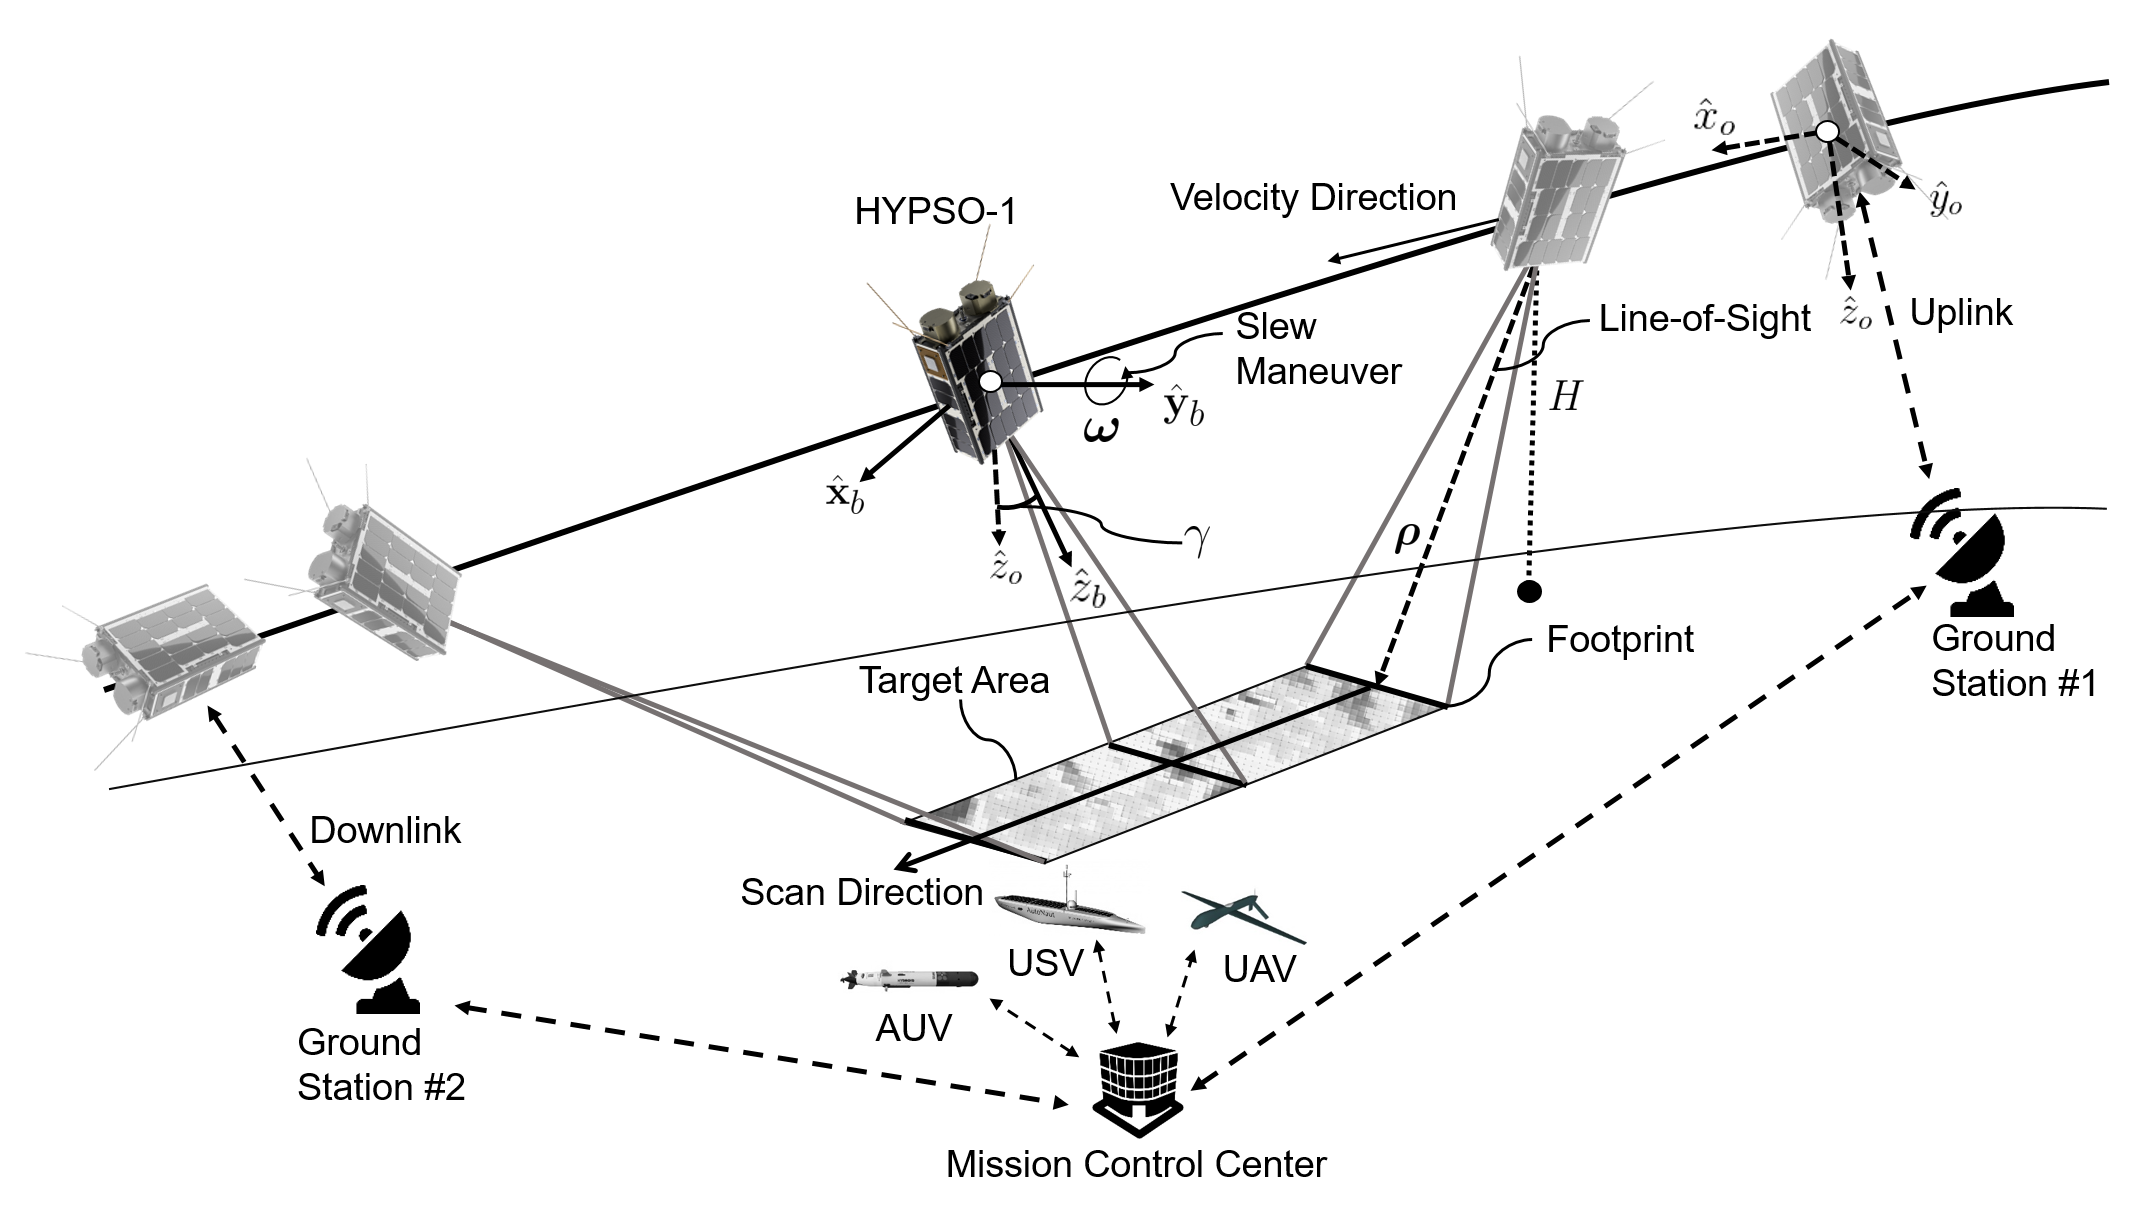
\includegraphics[width=160mm,angle=0]{figs/CONCEPT_HYPSO1.png}
    \caption{HYPSO-1 concept of operations}
    \label{fig:conops}
\end{center}
\end{figure*}
% \subsection{Requirements}\label{sec:requirements}
% \hl{Mariusz \\}
\subsection{Requirements}
In effort to support environmental monitoring, climate research and marine resource management, the objectives of the HYPSO-1 mission are to detect and monitor the spatial extent and motion of algal blooms; characterizing primary productivity; and observing other substances resulting from aquatic habitats as well as water pollution. Based on \cite{Ack16,Dic05, Mouroulis1998, Lancheros2018}, the key recommendations for ocean color remote sensing are:
\begin{enumerate}
    \item Image resolution should be better than $100 \hspace{3pt} \rm{m/pixel}$;
    \item Spectral resolution should be better than $10 \hspace{3pt} \rm{nm}$;
    \item SNR at Top of Atmosphere (ToA) should be greater than $ 100$;
    \item Data should be delivered to end users in less than 12 hours in general and less than 3 hours for HABs; and
    \item Revisit times to target should be at least 3 per day.
\end{enumerate}
Since HYPSO-1 mission is a single small-satellite but the first in a prospective constellation, we focus on working towards satisfying the recommendations 1), 2), 3) and 4). For 5), even though observations of the same target area in consecutive passes are possible, image quality is poor when viewing at large off-nadir angles thus mandating a constellation with multiple satellites to enable many revisits.
%We note that (5) may be artificially achieved if HYPSO-1 data is immediately combined with data from traditional satellites (e.g. Sentinel-3). 
% 
% The inference on algal blooms, especially if harmful, is typically not imminent from solely optical remote sensing \cite{IOCCG2014,IOCCGRep8}, requiring 
% simultaneous or near real-time in-situ measurements that provide data to identify/confirm the algae properties as well as estimating their propagation due to ocean currents and expansion/reduction in spatial extent. 

Monitoring the ocean from space requires cameras that capture enough light because the Earth's atmosphere weakens and scatters the water-leaving radiance \cite{Davis:02}, and most of the phytoplankton and algae typically reside at $10-15 \hspace{3pt} \rm{m}$ below the water surface \cite{IOCCG2014}. Such dark targets normally need tailored atmospheric correction schemes to retrieve the actual ground reflectance in the data \cite{Corson2008, Gao2009}.
% Furthermore, to mitigate the sun-glint effects that obscure the water-leaving radiance, observations should be made when solar zenith angle at the target is between $30-60 \hspace{3pt} \rm{deg}$ and the camera is tilted at an off-nadir viewing angle of $40 \hspace{3pt} \rm{deg}$ and sun-angle of $135 \hspace{3pt} \rm{deg}$ \cite{Kay2009}. 
\subsection{Imaging Trade-offs}
Many spectrometers can be integrated on aerial or space platforms \cite{Mouroulis2018, Wolfe1997}. In particular the pushbroom imager design is an attractive choice. It is able to obtain relatively good SNR since the hosting satellite moves in an approximately local linear track while the imager sequentially captures lines of cross-track pixels, each instantaneously contains dozens or hundreds of narrow spectral bands \cite{Fowler2014, VANE1993127}. 
  
From an orbit altitude, small sensor systems on small-satellites typically provide low instantaneous spatial resolution and SNR. A flexible performance factor and work-around is to improve the Sequential Ground Sampling Distance (SGSD). Here SGSD is taken to be the Euclidean distance between the centers of a reference pixel as seen from ground in two consecutive frames rather than the instantaneous ground distance between adjacent pixels which is commonly defined as the Ground Sampling Distance (GSD). The SGSD may be decreased by tilting the sensor or whole spacecraft while the camera is capturing images. This results in increased number of partially overlapping pixels that may be utilized by super-resolution techniques to improve the SNR and spatial resolution. 

Moreover, a suitable objective is be to map small specific target area(s) of interest that may be quickly revisited. This enables the use of an imaging system with high spectral resolution, a relatively narrow Field-of-View (FoV) and high camera frame rate which do not excessively compromise the SNR nor produce excessive amount of data to downlink. 
\subsection{Concept of Operations}
% Field campaigns with existing AUVs, that are sampling chl-a and characterizing ocean substances in the upper water column, are organized regularly in the Fr{\o}ya region in Mid-Norway, Western Norway as well as Svalbard \cite{Fossum19,fossum18,fossum18b}. The HYPSO-1 mission may provide the necessary macro-perspective and may alert ground operators to investigate specific areas of interest to support these campaigns. The existing AUVs and other assets that give point-to-point in-situ measurements or ground truth, such as from USVs and UAVs, shall be utilized for vicarious calibration and validation of the hyperspectral data \hl{[ref]}.
\begin{figure}[htbp]
  \begin{center}
    
\includegraphics[width=70mm,angle=0]{figs/trade-off chart.png}
    \caption{Diagram showing trade-offs. The extent of the gray pointers indicate the importance of each trade-off at the vertices. "$\otimes$" corresponds to favoured placement of the overall design selection.}
    \label{fig:trade-off}
\end{center}
\end{figure}
HYPSO-1 shall be launched into Sun-Synchronous Orbit (SSO) at an altitude of approximately $500 \hspace{3pt} \rm{km}$ and a LTAN/LTDN between 10:00-11:00 AM. The chosen orbit grants access to observe the Norwegian coastline in the morning during Spring and Summer seasons and also supports the local field campaigns. The particular choice of orbit is chosen as a trade-off between mainly the footprint size, image resolution, SNR, data latency and coverage to selected ground stations and target areas, as seen in Figure \ref{fig:trade-off}. Moreover, the advantage of SSO is that the satellite passes over any given point on the Earth’s surface at approximately the same local sidereal time. Combined with appropriate viewing angles during imaging, the observation windows are also safe from detrimental sun-glint effects \cite{Kay2009}.
% Because ocean color phenomena such as primary productivity are more prevalent in the morning or mid-day, the launch LTAN/LTDN is chosen to be between a strict window of 10:00-11:00 AM. The chosen LTAN/LTDN, combined with appropriate viewing angles during imaging, also reduces the detrimental sun-glint effects during the particular seasons. 

% At a significant orbital speed, a push-broom hyperspectral imager (HSI) captures narrow 2D lines with up to hundreds of spectral bands to observe both organisms and matter in the upper water column. Images are created by georeferencing and combining a group of scan lines. Sufficiently high spatial and spectral resolution may be utilized to infer the chemical or biological composition and concentrations in the upper water column \cite{Geir2011}. 
Presented and summarized in Figure \ref{fig:conops}, the HYPSO-1 mission enables five essential capabilities:
\begin{enumerate}
    \item After receiving telecommands and necessary updates (e.g. camera configurations) from a nearby ground station, HYPSO-1 shall orient its hyperspectral imager to quickly scan a predefined target area on the sub-mesoscale, i.e. no larger than $100 \hspace{3pt} \rm{km}$ by $100 \hspace{3pt} \rm{km}$. 
    % The hyperspectral imager shall be configured to have less than $10 \hspace{3pt} \rm{nm}$ spectral resolution.
    % % Evidently, scenarios with presence of thick cloud-cover or strong sun-glint effects entails abortion, avoidance or relocation of imaging to other desired targets.
    \item To achieve a SGSD better than $100 \hspace{3pt} \rm{m/pixel}$ while acquiring hyperspectral lines at a high frame rate, HYPSO-1 shall rotate the camera footprint incrementally backwards with respect to the scan direction by executing a slew maneuver. 
    % This also results in an increased number of partially overlapped pixels as compared to when imaging at nadir and more data is collected about the optical path through the atmosphere by varying the camera's orientation. 
    The rotation shall nominally start at $20 \hspace{3pt} \rm{deg}$ off-Nadir viewing angle. 
    % Consequently this may give the desired image resolution of potentially better than $100 \hspace{3pt} \rm{m}$ if the attitude accuracy requirement is achieved. 
    % Prior to imaging, the spacecraft shall be oriented to the starting angle and have sufficient time for the sensor biases and estimator initialization to stabilize.
    % This means that an angular rate of $0.7025 \hspace{3pt} \rm{deg/s}$ during $53.4 \hspace{3pt} \rm{s}$ to cover a $42.44 \hspace{3pt} \rm{km}$ ground track.
    % % meaning at a slew rate of $0.7025 \hspace{3pt} \rm{deg/s}$ and image acquisition for approximately 57 seconds. 
    % 0.011459
    % \item In conjunction with hyperspectral imaging, a Red-Green-Blue (RGB) camera shall instantaneously cover the entire target area within a single image with appropriate FoV. The RGB image shall be taken mid-way of the HSI scan, meaning when the spacecraft is oriented at Nadir during the slew maneuver.
    \item The images are immediately processed onboard to reduce the data size in order to alleviate the power budget and speed up the data delivery to end users.
    \item 
    % Available nearby ground stations with S-band antennas enable operators to quickly upload updates on mission parameters (e.g. camera configuration, settings, spacecraft angular rate) before image acquisition. 
    For quick downlink capability, the ground station network consists of the S-band ground stations at NTNU, KSAT Svalbard, Norway, and KSAT Puertollano, Spain. The NTNU Mission Operations Center in Trondheim, Norway, also operates its autonomous aerial, surface and underwater vehicles.
    \item If in the proximity of the target area, the UAVs, ASVs or AUVs may be quickly guided towards information-rich parts in a spontaneous fashion given a quick downlink from HYPSO-1. 
    % Aerial drones with hyperspectral imaging capability, may be dispatched on-demand and collect data at higher spatial resolution. Additionally, USVs, AUVs and/or aquatic buoys will physically sample the water surface to verify its chemical and physical composition.
\end{enumerate}
\subsection{Capabilities}
\subsubsection{Imaging Modes}
The hyperspectral imager shall have the following three modes:
\begin{itemize}
    \item High-resolution mode: enables high image resolution with a narrow-FoV and high frame rate setting;
    \item Wide FoV mode: enables medium image resolution and is used for scanning larger target areas; and
    \item Diagnostics mode: may offer low spatial resolution but shall have high spectral resolution. This mode shall be used for in-orbit calibration and characterization.  
\end{itemize}
\subsubsection{Attitude Determination \& Control System}
Practically obtaining SGSD of less than $100 \hspace{3pt} \rm{m}$ requires an ADCS that provides stable attitude tracking performance during the slew maneuver or otherwise when pointing \cite{Gue16, agrawal2009, Santandrea2013}. During the slew maneuver the attitude accuracy of better than $\pm 0.00535 \hspace{3pt} \rm{deg}$ should be achieved. Without scheduled imaging, then an ADCS mode for coarse attitude determination mode can be used instead to decrease power consumption.
\subsubsection{On-board Image Processing}
The on-board image processing on HYPSO-1 shall primarily reduce the size of the data and extract useful information for end users. Key algorithms shall be implemented in a modular image processing architecture that shall ease the satellite operations and provide tailored information with low data latency. This also requires a fast processing unit. The main capabilities are
\begin{itemize}
    \item Lossless compression to reduce data size;
    \item Radiometric, spectral and geometric corrections to produce more accurate data;
    \item Image registration and geo-referencing for structuring the data;
    \item Super-resolution algorithms to utilize the SGSD and achieve better than $100 \hspace{3pt} \rm{m/pixel}$ image resolution; and
    \item Dimensionality reduction, target detection and classification to extract only the spatial and spectral information of interest, thereby resulting in a significant reduction in data size and latency.
\end{itemize}
For the latter, the downloaded data product shall be complemented and validated by other available remote sensing data in synergy or with modeling and simulation tools to provide supporting information \cite{Lapadatu2019}.
% \subsection{Data Validation (TENTATIVE)}
% \hl{Mariusz, Sivert, Joe \\}

% The initial phase of the mission requires ground-based algorithms that fuse information from satellites, autonomous vehicles, and ocean models in order to improve the accuracy of target detection using hyperspectral imaging. 
% Simultaneous co-temporal observations from one or more UAVs' hyperspectral imaging capability and ground-truth provided by in-situ platforms near the ocean surface can then be used to accurately measure and validate the features of interest at a much finer scale in the upper water column, and without the distortion from the atmosphere or being limited by cloud cover. 
% Simulation tools may be utilized for simulating how different geophysical variables, such as chl-a, translate to radiance across a chosen spectral range. How the medium around it affects the values as well as estimated temporal changes based on ocean models. 
% Both the simulations and data fusion will provide insight into how the atmosphere affects the ground radiometry for various wavelengths, viewing or look angles, and solar zenith angles \cite{Lapadatu2019}.
% The robotic agents, such as hyperspectral imaging aerial drones, may be dispatched on-demand to the target area observed by HYPSO-1 and collect data at higher spatial resolution. Additionally, USVs, AUVs and/or aquatic buoys will physically sample the water surface to verify its chemical and physical composition. 
% The inference on algal blooms, especially if harmful, is typically not imminent based on only direct optical observations \cite{IOCCG2014,IOCCGRep8}. 
% Simultaneous or consecutive in-situ measurements may provide data to identify/confirm the algal blooms species’ properties and estimate their propagation with ocean currents. 
% This means that aerial, surface or underwater vehicles in vicinity may be guided towards data-rich parts of the target area in near real-time.
% \subsection{Optical Remote Sensing Limitations (TENTATIVE)}
% \hl{Mariusz, Roger \\}
% Key limitations in for optical observations of are mainly due to nature and are uncontrollable, these being 
% \begin{enumerate}
% \item cloud cover;
% \item sun-glint;
% \item white caps or turbulent water; 
% \item excessive mixing of river sediments (e.g. CDOM and SM) and chlorophyll;
% \item water-depth penetration;
% \item revisit times;
% \end{enumerate}
% Cloud cover is significantly detrimental to optical EO, and may render the temporal sampling or revisits for any given region being much less than intended with a chosen orbit. This is mainly due to the following factors: (a) complete and dense cloud cover renders the target unobservable from space; (b) scattered clouds cause reflection of sunlight, not necessarily directly in the camera's FoV, which interferes with water-leaving radiance and water-reflected radiance collected by the sensor; (c) thin clouds cause reflection of water-leaving and water-reflected radiance and not everything will go through the atmosphere and reach the sensr, thus causing lower SNR. 
% Especially in the vicinity of the Arctic, this is a particularly limiting factor, where cloud cover is prominent throughout the year. To handle the cloud cover problem, the satellite may be commanded to look at other target areas and that the ground segment closely follows the weather prediction models or be continuously updated on images from available public sources. In case of an algal bloom event with complete cloud cover, the only mitigation would be to use in-situ agents to investigate the target. Also, if there are scattered clouds at a fixed target area to be revisited or partially covering an algal bloom, the spacecraft may abstain from Nadir mode and utilize its attitude control to point away from the cloud cover.
% White caps or turbulent water as well as excessive mixing with sediments may
% completely or partially render the presence of preferred targets such as algal blooms unobservable. The latter would require very high spectral resolution to distinguish the constituents in the water. 
% The revisit times to specifically chosen targets are also at stake due to the orbit repeat cycles at best being a few days. Flexible pointing capability, where the satellite is equipped with actuators that provide sufficient torque, may enable observing the same target area in multiple passes at the cost of degraded image quality since the range/optical path through the atmosphere would be longer. 
% \subsection{Risk Assessment (TENTATIVE)}
% \hl{Evelyn, Roger, Mariusz \\}

% \begin{enumerate}
% \item Cloud cover over
% relevant target
% areas \cite{Braaten2019}: To ensure the utility of HYPSO-1 during cloud cover at
% specific target areas, it shall be able to observe elsewhere upon careful study by the Ground
% Segment and User Segment. Alternate target areas shall be investigated based on users feedback.
% Pointing capability will also allow for flexibility whenever clouds are scattered nearby a target area
% and requires rigorous simulations to avoid a missed opportunity at the cost of the satellite’s power
% budget. Careful monitoring with near real-time data on weather prediction and ocean models will be
% implemented in the operations planning. In case of simultaneous algal bloom and thick cloud cover there is no other way than to wait and look elsewhere.
% \item No observable algal blooms throughout operational phase: Based on optics and sensor characteristics it is
% difficult to say whether the payload may be able to
% produce images even if the presence of algal blooms
% optical characteristics are strong by visual inspection
% on the ground. Related to this are also i) mismatch in
% orbit pass with algal bloom or ii) water conditions do
% not favor the production of algae in that particular
% year at planned locations. To ensure the utility of the
% mission then other ocean color events may be
% observed such as river plumes, sea ice, water
% turbidity that are more predictable in nature, thus
% enabling data products to the general ocean color
% community.
% \item The developed HSI
% prototype does not
% meet the expectations of the
% end users: 
% \item Failure caused by
% cosmic radiation: Contemporary, cutting edge COTS electronic
% devices can be vulnerable in terms of in-orbit radiation environment. To mitigate this risk several
% design choices have been addressed (i) active radiation hardened supervisory circuit to detect and isolate errors caused by radiation,
% (ii) hardware protection against SEL, (iii) EDAC, TMR and scrubbing mechanisms across the system to address SEE, (iv) utilization of radiation tested parts or parts
% with flight heritage as much as possible, (v) radiation shielding against TID.
% \item Power consumption
% too high: The possibility of a higher than expected power
% consumption exists and can lead to unbalanced satellite power budget. Mitigation actions were undertaken by specifying conservative power budget. Also, to make
% sure the power consumption falls within expected
% range a detailed monitoring is provided. The
% mechanism of controlling the unit performance is
% also implemented, therefore once required, the
% hardware may be switch into slower but less power-consuming mode.
% \end{enumerate}
\section{Pushbroom Hyperspectral Imager} \label{sec:hsi}
\begin{figure*}[htbp]
  \centering
      
\includegraphics[width=0.7\textwidth]{figs/optics.png}
  \caption{Optical diagram of the pushbroom hyperspectral imager based on \cite{Sigernes18}.}
	\label{fig:optics}
\end{figure*}
% \textcolor{blue}{Contribution (2): "We present a COTS-assembled hyperspectral imager with high spectral resolution and efficiency designed for the HYPSO-1 mission and is based on \cite{Sigernes18}. We present the chosen components for the design that satisfy objectives of observing algal blooms, and show how SNR may be increased by binning operations." Key points to keep in mind while writing this section:
% \begin{itemize}
%     \item How does the proposed HSI work?
%     \item How is it performing from space on HYPSO-1?
% \end{itemize}}
\subsection{Optics}\label{sec:optics}
Emerging commercial off the shelf (COTS) products that are smaller in size make hyperspectral imaging accessible, flexible and affordable \cite{Sigernes18}. Such low-cost pushbroom cameras may in principle be designed and integrated into small-satellites.
\begin{figure}[htbp]
  \centering
      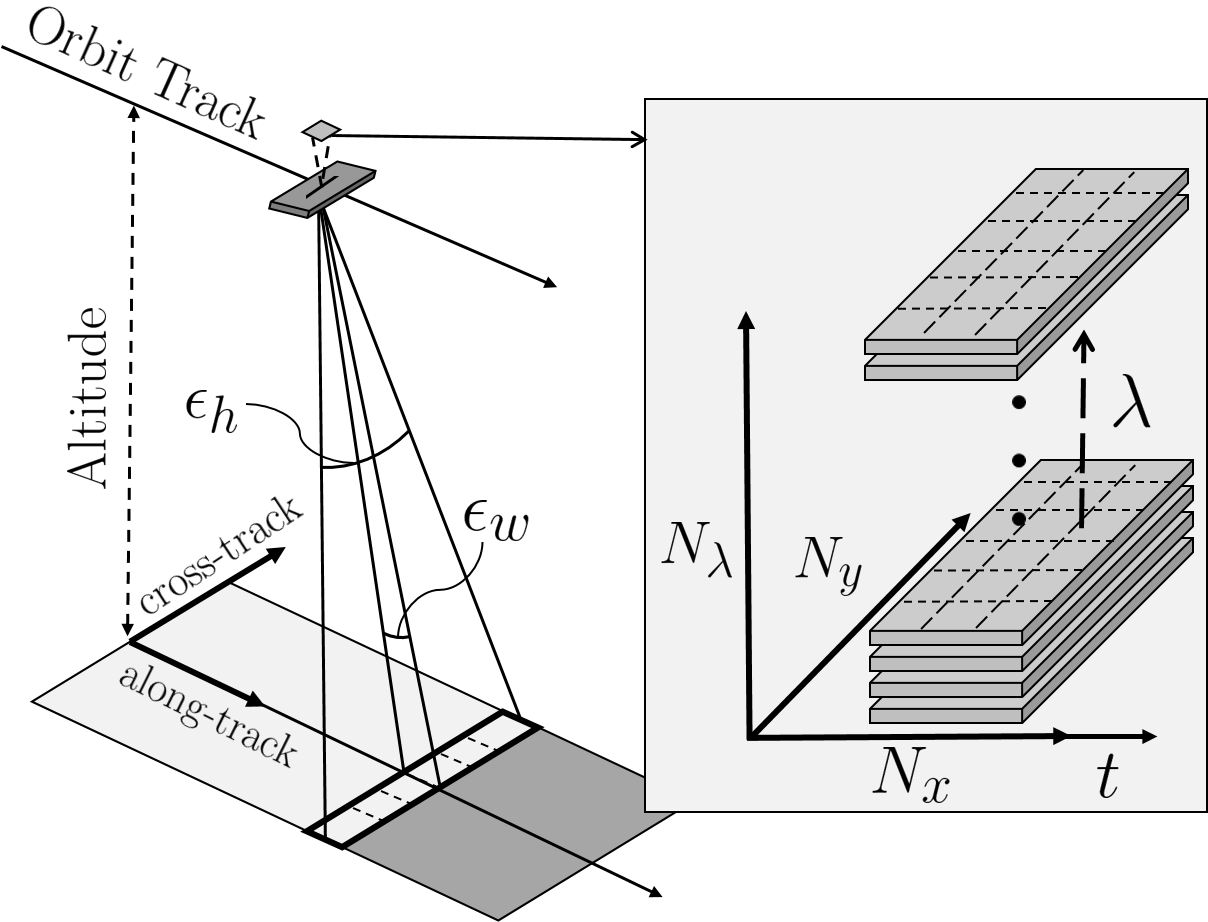
\includegraphics[width=0.45\textwidth]{figs/pushbroom_scanning.png}
  \caption{Data acquisition with pushbroom hyperspectral imaging.}
	\label{fig:push_scan}
\end{figure}
% Figure \ref{fig:push_scan} shows a satellite-based pushbroom hyperspectral imager collecting lines of cross-track pixels and spectral information, eventually forming a datacube. 
Figure \ref{fig:optics} shows the optical diagram of a center cross-section of the instrument parallel to the refraction axis. The components are: (i) front lens with aperture diameter $D_0$ and focal length $F_0$; (ii) entrance slit with dimensions $w_{\text{slit}}$ and $h_{\text{slit}}$ that are slit width and height, respectively; (iii) collimator lens with aperture diameter $D_1$ and focal length $F_1$; (iv) grating that receives the incoming light at angle $\alpha=0^{\circ}$ and diffracts the light at angle $\beta$ measured from the grating normal; and (v) detector lens with aperture diameter $D_2$ and focal length $F_2$. Finally, (vi) is the detector. The horizontal and vertical components of the FoV, $\epsilon_w \times \epsilon_h$, are found from the slit width and height as
\begin{subequations}
\begin{align}
\tan{\left(\frac{\epsilon_{w}}{2}\right)} &= \frac{w_{\text{slit}}}{2F_0}, \label{eq:fov_x} \\
\tan{\left(\frac{\epsilon_{h}}{2}\right)} &= \frac{h_{\text{slit}}}{2F_0}. \label{eq:fov_y}
\end{align} 
\end{subequations}

Assuming no loss of light transmission within the spectrometer from the front to the exit plane, the etendue is expressed as
\begin{equation}
G = \pi \frac{D_0^2}{4 F_0^2}\cos(\beta_c) w_{d} h_{d},
\end{equation}
\noindent where
\begin{subequations}
\begin{align}
h_{d} &= h_{\text{slit}}\frac{F_2}{F_1}, \label{eq:effective_height}\\
w_{d} &= \frac{w_{\text{slit}}F_2}{\cos(\beta_c)F_1} \label{eq:effective_width},
\end{align}
\end{subequations}
\noindent and $\beta_c$ is the diffraction angle at center wavelength $\lambda_c$ \cite{Lerner2006}. It is assumed that $\beta_c\approx\beta(\lambda)$ for all $\lambda$.
% The horizontal and vertical magnification of entrance slit image

The bandpass $BP$ for the optical system, or the recorded Full Width at Half Maximum (FWHM) of a monochromatic spectral
line, and is a measure of the instruments ability to separate adjacent spectral lines in the
spectrogram. Assuming no degradation due to aberrations and diffraction effects, the optical bandpass may be approximated as
\begin{align}
BP &\approx\frac{g w_{\text{slit}}}{\kappa F_1}, \label{eq:bp}
\end{align}
\noindent where $g$ is the grating groove spacing and $\kappa$ is the spectral order \cite{Lerner2006}. 
% For an emission with finite spectral bandwidth such as fluorescent light, in real-life the bandpass is also a function of the natural spectral bandwidth of the emitting source and the limiting resolution of the instrument, where the latter usually has a minuscule effect.
\subsection{Detector}
 $N_x$ lines with $N_y$ and $N_\lambda$ pixels each are collected sequentially during each camera integration time $\Delta t$, to form a threedimensional datacube. $N_y$ is the total number of spatial pixels perpendicular to the scan direction and $N_{\lambda}$ is the total number of pixels along the spectral dimension, cf. Figure \ref{fig:push_scan}. It is assumed that $\Delta t=1/FPS=\tau +\delta t$ is the associated camera integration time where $FPS$ is the frame rate, $\tau$ is the camera exposure time and $\delta t$ is the camera read-out time.
\begin{figure}[htbp]
  \centering
      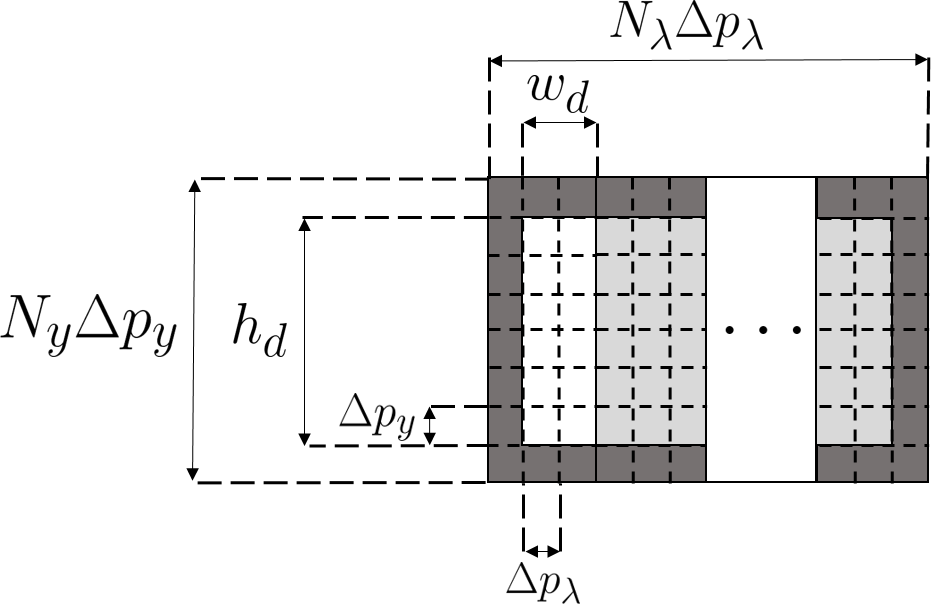
\includegraphics[width=0.4\textwidth]{figs/fad.png}
  \caption{Detector plane with $h_d$ and $w_d$ being the vertical and horizontal magnification of the entrance slit image. The camera's mechanical layout may block some of the light as shown by the darkest gray regions.}
	\label{fig:fad2}
\end{figure}
The rounded up amount of illuminated pixels in per magnified slit image, as shown in Figure \ref{fig:fad2}, are approximately
\begin{subequations}
\begin{align}
    N_{h} = \frac{h_d}{\Delta p_y}, \\
    N_{w} = \frac{w_d}{\Delta p_\lambda},
\end{align}
\end{subequations}
\noindent where $\Delta p_\lambda$ and $\Delta p_y$ are the width and height of a pixel, respectively.

With the ability to bin pixels, photon-electrons are gathered from adjacent pixels to create one merged pixel with higher SNR at the cost of reduced spectral or spatial resolution. The signal increases proportionally with the square root of number of binning operations $B_{\lambda}$ in the spectral direction or $B_{y}$ in the vertical spatial direction. 
\subsection{Signal-to-Noise Ratio}
The photon flux into the detector may be written as
\begin{equation}
\dot{\Phi}(\lambda) = L(\lambda)\eta_0 \eta_1 \eta_{G}(\lambda) \eta_2 G \lambda\frac{ BP}{h_{\text{planck}}c}, \label{eq:photons}
\end{equation}
\noindent where $L(\lambda)$ is the radiance as a function of wavelength reaching the sensor, $\eta_0, \eta_1, \eta_2$ are the optical efficiencies of the front, collimator and detector lenses respectively, $\eta_G$ is the grating efficiency, $c$ is the speed of light, and $h_{\text{planck}}=6.62607015\times10^{-34}$ $\rm{Js}$ is the Planck constant. 

The number of photons converted to electrons in each pixel is
\begin{equation}
c_{\text{electrons}} = \frac{\eta_{\text{QE}}(\lambda)\dot{\Phi}(\lambda)\tau}{N_{w}N_{h}}, \label{eq:photons2}
\end{equation}
\noindent where $\eta_{\text{QE}}(\lambda)$ is the quantum efficiency of the detector. Assuming that $c_{\text{electrons}}$ has a Poisson probability distribution, then the SNR in one unbinned pixel is
\begin{align}
SNR_{[1, 1]} 
&=\frac{c_{\text{electrons}}}{\sqrt{c_{\text{electrons}} + c_{\text{dark}}+c_{\text{read-out}}^2+c_{\text{dig}}^2}}.  \label{eq:snr}
\end{align}
\noindent where $c_{\text{dark}}=i_{\text{dark}}\Delta t$ is represented with a Poisson probability distribution, while $c_{\text{read-out}}$ and $c_{\text{dig}}$ are assumed to have Gaussian probability distribution with zero mean \cite{Moses2012, Skauli2011}. $i_{\text{dark}}\Delta t$ is the average shot noise registered due to dark current $i_{\text{dark}}$, $c_{\text{read-out}}$ is the standard deviation of electrons due to the sensor read-out circuits, and $c_{\text{dig}}=c_{\text{electrons},\text{max}}/(2^{b}\sqrt{12})$ is the standard deviation of digitization (or quantization) noise where $c_{\text{electrons},\text{max}}$ is the well depth of electrons and $b$ is the Analog-to-Digital Converter (ADC) bit depth.

To match the optical bandpass then we must bin $B_\lambda=\ceil{N_w}$ pixels in the spectral direction where $\ceil{\cdot}$ means rounding up to an integer, rendering the SNR in a $[\ceil{N_w}, 1]$ window to be $SNR_{[\ceil{N_w}, 1]} \approx \sqrt{N_w}SNR_{[1,1]}$. Binning may also be applied for the spatial pixels. In particular, if large distances are covered during each camera exposure time such as for HYPSO-1, the partial overlap of frames in the along-track direction may be utilized to predict the benefits of super-resolution algorithms.

\subsection{Payload Design} \label{sec:payload-hsi}
HYPSO-1's payload, shown in Figure \ref{fig:HSI}, is built with mainly COTS products from Thorlabs and Edmund Optics and a few 3D-printed parts \cite{Sigernes18}. The design provides a spectral range in the visual and near-infrared part of the spectrum and bandpass of $3.33 \hspace{3pt} \rm{nm}$ which fulfills HYPSO-1 mission requirements to observe algal blooms and primary productivity. In theory, the f-numbers should be equal to maximize the light throughput in the optics, however these are set to $F_0/\#=F_1/\#=2.8$ and $F_2/\#=2$ to avoid stray light effects. The instrument's specifications and performance are given in Table \ref{tab:optics}.
\begin{figure}[tbhp]
  \begin{center}
    %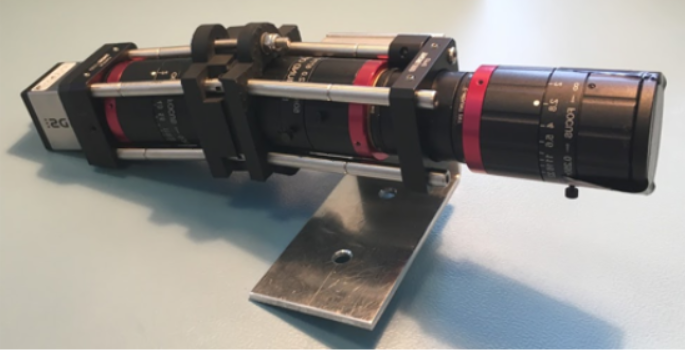
\includegraphics[width=70mm,angle=0]{figs/HSI_v6.PNG}
    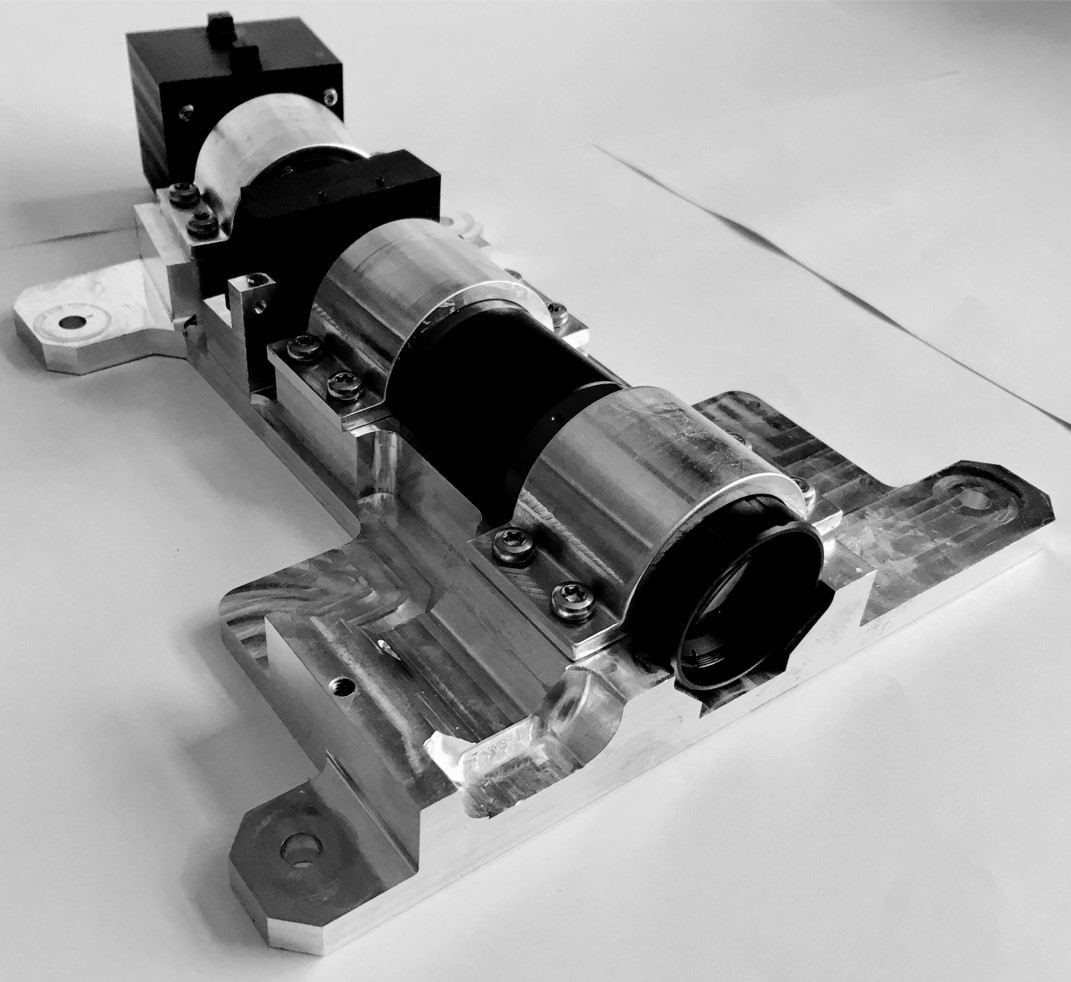
\includegraphics[width=60mm,angle=0]{figs/HSI.jpg}  %more options in figs/mech folder
    \caption{Hyperspectral imager payload assembled for CubeSat integration}
    \label{fig:HSI}
\end{center}
\end{figure}

The chosen sensor is the SONY IMX249 mounted in an industrial camera head from The Imaging Source Europe GmbH. It has a reported well depth of about 33022 $e^{-}$, equivalent to a maximum SNR of approximately $181.6$ or $45.2 \hspace{3pt} \rm{dB}$ per pixel if not binned.The detector enables a maximum frame rate of up to $FPS=47$, but due to constraints on the data throughput the practical FPS setting is governed by the number of binning operations, subsampling of pixels and the chosen window of pixels, commonly named as the Area of Interest (AoI).
\begin{table}[htbp]
	\caption{Hyperspectral imager specifications}
	\label{tab:optics}
	\centering
			\begin{tabular}{l l}
				\hline
				Parameter & Value \\
				\hline 
				FoV $\epsilon_w \times \epsilon_h$ &	$0.0564^{\circ} \times 7.8826^{\circ}$  \\
				$F_0=F_1=F_2$ & 50 $\hspace{3pt} \rm{mm}$ \\
				$F_0/\#=F_1/\#$ & 2.8  \\
				$F_2/\#$ & 2 \\
				$D_0=D_1$  & 17.9 $\hspace{3pt} \rm{mm}$ \\
				$D_2$ &  25 $\hspace{3pt} \rm{mm}$ \\
				Slit width $w_{\text{slit}}$ & 50 $\hspace{3pt} \mu\rm{m}$ \\
				Slit height $h_{\text{slit}}$ & 7 $\hspace{3pt} \rm{mm}$ \\
				Optical efficiency $\eta_{0}=\eta_{1}=\eta_{2}$ & $0.8$ \\
				Grating efficiency $\eta_{G}$ @$500\hspace{3pt} \rm{nm}$ & 0.73 \\
				Spectral order $\kappa$ & 1 \\
				Groove spacing $g$ & 3333.33 $\hspace{3pt} \rm{nm}$ \\
				Diffraction angle $\beta_c$ & 10.37$^{\circ}$ \\
				Pixel size $\Delta p_\lambda=\Delta p_y$ & $5.86 \hspace{3pt} \mu\rm{m}$ \\
				% Full detector resolution & $1936 \times 1216 \hspace{3pt} \rm{pixels}$ \\
				Usable detector resolution & $1936 \times 1194  \hspace{3pt} \rm{pixels}$ \\
				Quantum efficiency $\eta_{QE}$ @$500\hspace{3pt} \rm{nm}$ & 0.77 \\
				Spectral range &  $271-1006 \hspace{3pt} \rm{nm}$ \\ 
			    Bandpass $BP$ & $3.33 \hspace{3pt} \rm{nm}$ \\
				Dark current $i_{\text{dark}}$ & $0.95 \hspace{3pt} \rm{e}^{-}/\rm{s}$ \\
				Read-out noise $c_{\text{read-out}}$ & $6.93 \hspace{3pt} \rm{e}^{-}$ \\
				Quantization noise $c_{\text{dig}}$ & $2.33 \hspace{3pt} \rm{e}^{-}$ \\
				Max. SNR per pixel (unbinned) & $181.6$ ($45.2 \hspace{3pt} \rm{dB}$) \\
			    ADC bit-depth & $12\hspace{3pt}\rm{bits}$ \\
			 %   AoI & $1280 \times 720$ pixels \\
			 %  Binning $B_\lambda \times B_y$ & $6 \times 1$ \\
			 %  Subsampling & 2 \\
  		    % FPS $\zeta$ & Up to $47$ \\
				\hline
				\end{tabular}
\end{table}
% \begin{figure}[H]
%   \centering
%       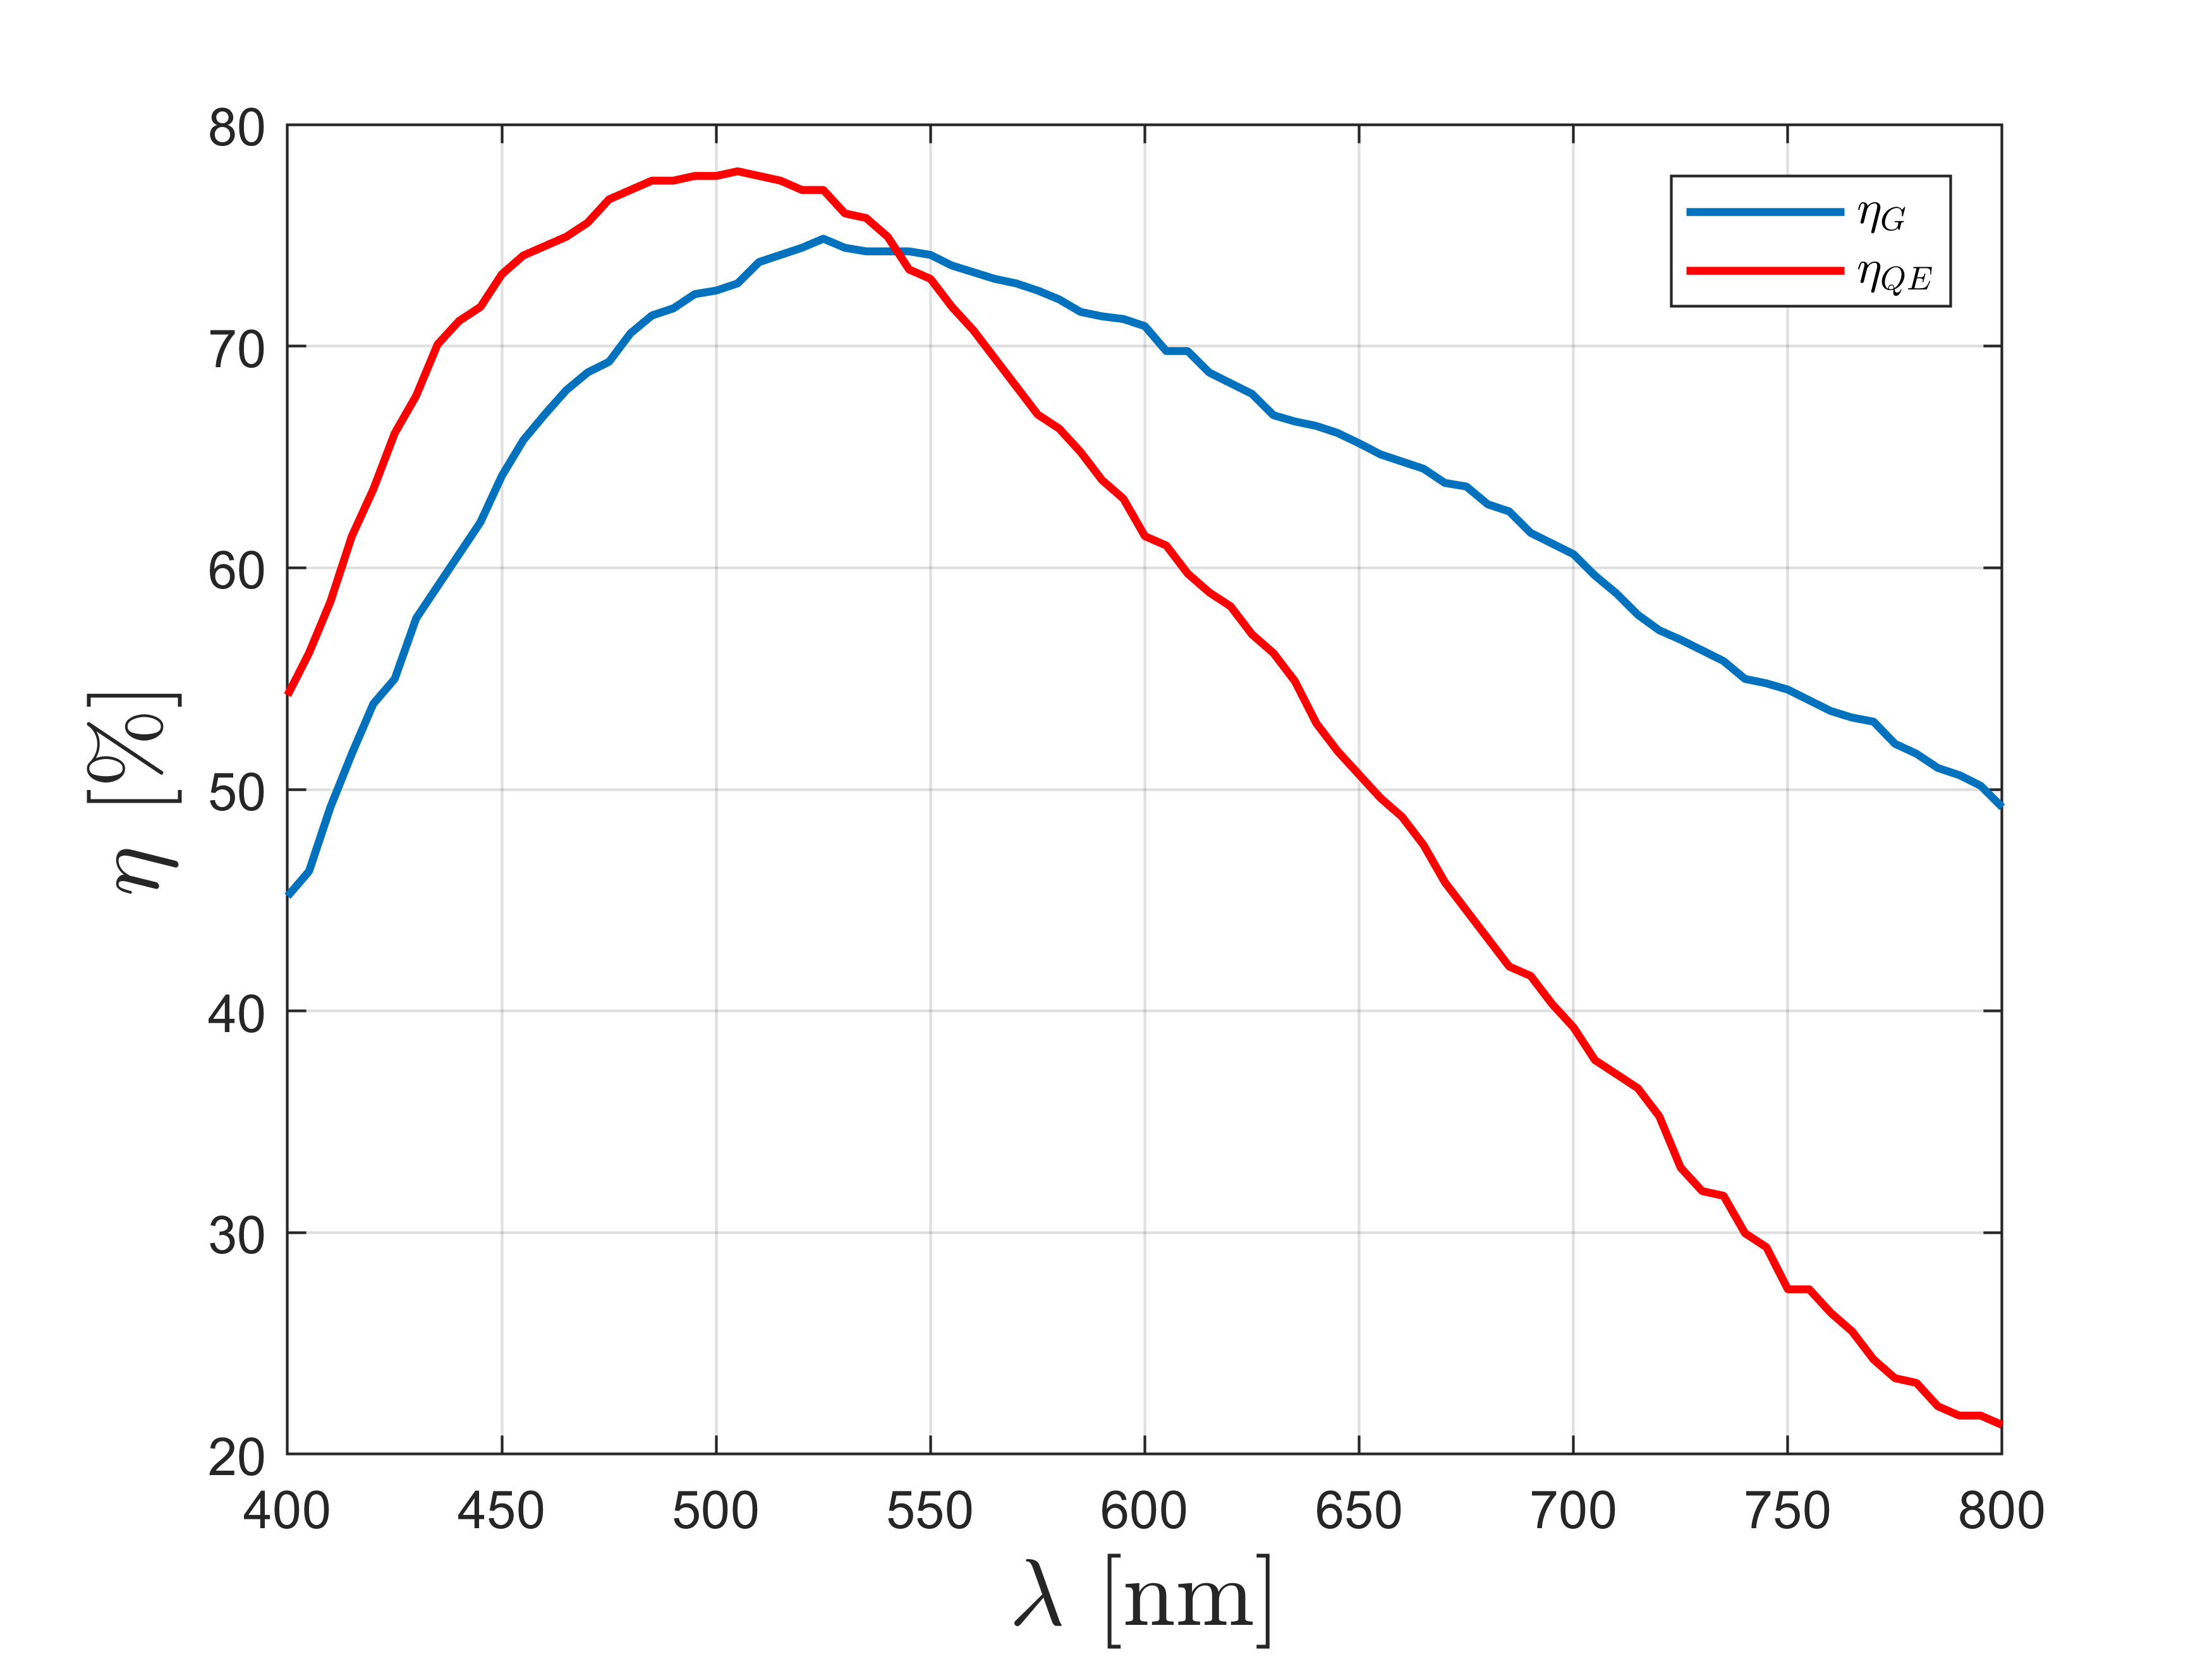
\includegraphics[width=0.45\textwidth]{figs/optical_eff.png}
%   \caption{Efficiencies for the grating and sensor SONY IMX249 across the spectral range.}
% 	\label{fig:optical_eff}
% \end{figure}

\section{Sampling} \label{sec:sampling}
\subsection{Geometry}
Shown in Figure \ref{fig:conops}, 
% the origin of the body frame is with the coordinate system defined by triad vectors $\hat{\mathbf{y}}_b$, $\hat{\mathbf{x}}_b$, and $\hat{\mathbf{z}}_b$ that in respective order point along the largest to the smallest principal inertia axes. 
the triad axes $\hat{\mathbf{x}}_b$, $\hat{\mathbf{y}}_b$ and $\hat{\mathbf{z}}_b$ represent the body frame that rotates in orbit. The refraction axis of the hyperspectral imager  is mounted along the $\hat{\mathbf{z}}_b$ axis, the slit height $h_\text{slit}$ is mounted along the $\hat{\mathbf{y}}_b$ axis and the slit width $w_\text{slit}$ is mounted along the $\hat{\mathbf{x}}_b$ axis. The satellite's orbit frame where $\hat{\mathbf{x}}_o$ points along the velocity vector (along-track), $\hat{\mathbf{y}}_o$ points towards the negative orbit normal vector (cross-track), $\hat{\mathbf{z}}_o$ represents the nadir vector which is aligned with the position vector defined in the Earth-Centered-Inertial (ECI) frame. 
% The 2-D reference frame of a pixel on ground is represented with $\Delta x$ and $\Delta y$, being in-track and cross-track resolution respectively.
The rotation of the satellite body relative to the orbit may be represented by the Euler angles $\phi$, $\theta$ and $\psi$ which are the roll, pitch and yaw angles. In addition, the absolute angle between the Line-of-Sight (LOS) vector $\boldsymbol{\rho}$ and $\hat{\mathbf{z}}_o$, is defined as the viewing angle $\gamma$.
% \begin{align}
% \gamma &=\cos^{-1}\left(\frac{1}{\sqrt{\sec^2(\theta)+\tan^2(\phi)}}\right)
% \end{align}
% 
The angular velocities about the satellite body frame, as measured by on-board gyroscope sensors, are represented by $\omega_x$, $\omega_y$, and $\omega_z$. 

% The transformation is undefined for $\theta = \pm \frac{\pi}{2} \pm q \pi$ where $q$ is an integer.\footnote{In practice, it is assumed that the singularity is avoided by imposing $\vert\theta\vert<\frac{\pi}{2}$ during a slew maneuver about the $\hat{\mathbf{y}}_b$ axis as the concerned remote sensing targets are beneath the orbit track and not at or beyond the Earth's horizon.}
The hyperspectral imager's instantaneous footprint, expressed in horizontal and vertical components, are
% \begin{subequations}
% \begin{align}
% P_{w} &= H\sin\Big(\frac{\epsilon_{w}}{2}\Big)\sec\phi\sec\theta \Bigg(\sec\Big(\theta+\frac{\epsilon_w}{2}\Big)\notag\\&+\sec\Big(\theta-\frac{\epsilon_w}{2}\Big)\Bigg), \\
% P_{h} &= H\sin\Big(\frac{\epsilon_{h}}{2}\Big)\sec\theta\sec\phi\Bigg(\sec\Big(\phi+\frac{\epsilon_h}{2}\Big)\notag\\&+\sec\Big(\phi-\frac{\epsilon_h}{2}\Big)\Bigg),
% \end{align}
% \end{subequations}
\begin{subequations}
\begin{align}
P_{w} &= H\sec\phi\bigg(\tan\Big(\theta+\frac{\epsilon_w}{2}\Big)-\tan\Big(\theta-\frac{\epsilon_w}{2}\Big)\bigg), \\
P_{h} &= H\sec\theta\bigg(\tan\Big(\phi+\frac{\epsilon_h}{2}\Big)-\tan\Big(\phi-\frac{\epsilon_h}{2}\Big)\bigg),
\end{align}
\end{subequations}
\noindent which are transformed to the along-track and cross-track components of a central pixel as
\begin{subequations}
\begin{align}
\delta x &\triangleq \cos(\psi)P_{w}+\sin(\psi)\frac{P_{h}}{N_{y}}, \label{eq:footprint_x}\\
\delta y &\triangleq \cos(\psi)\frac{P_{h}}{N_{y}}-\sin(\psi)P_w. \label{eq:footprint_y}
\end{align}
\end{subequations}
Ground-projected pixels near the edge of the swath are elongated compared to the central pixel. Along with effects from Earth curvature, this distortion is known as the "bowtie effect" which may be corrected in image processing \cite{Richards1999, Sayer2015}. We note that the ground pixel size is relatively small (i.e. on a meter-scale) and the combination of high frame rate and narrow FoV renders the pixel elongation and the Earth curvature as seen per pixel to be practically negligible.
\subsection{Spatial Resolution}
Using Eqs. (\ref{eq:footprint_x}) and (\ref{eq:footprint_y}), then the spatial resolution in a pixel acquired during exposure time $\tau$, as shown conceptually in Figure \ref{fig:push_scan}, are expressed in along-track and cross-track components as
\begin{subequations}
\begin{align}
    \Delta x=\delta x+v_{p,x}\tau, \label{eq:spatial1_x} \\
    \Delta y=\delta y +v_{p,y}\tau, \label{eq:spatial1_y}
\end{align}
\end{subequations}
\noindent where $v_{p,x}$ and $v_{p,y}$ are the along-track and cross-track pixel speed as measured on ground
\begin{subequations}
\begin{align}
    v_{p,x} & \triangleq v_{o}
+\dot{\theta}H-\dot{\psi}H\tan(\phi), \label{eq:rotational_vel1} \\
    v_{p,y} & \triangleq -\dot{\phi}H+\dot{\psi}H\tan(\theta), \label{eq:rotational_vel2}
\end{align}
\end{subequations}
\noindent with $v_o$ being the speed of the satellite as measured on ground. 
% The Earth ground speed $v_g$ results in moving features in an image pixel due to the Earth's rotational rate and decreases with higher geodetic latitude of the target area. The Relative Ground Shift (RGS) during a camera exposure time takes into account the relative motion between moving footprint and ground and may be determined by adding the Earth surface speed in the along-track and cross-track distances covered such that $(v_{p,x}-v_{g,x})\tau $ and $(v_{p,y}-v_{g,y})\tau $, respectively. RGS is indicative of motion blur and determines how much a pixel and a surface feature has shifted on ground during an exposure.
\begin{figure}[htbp]
  \begin{center}
    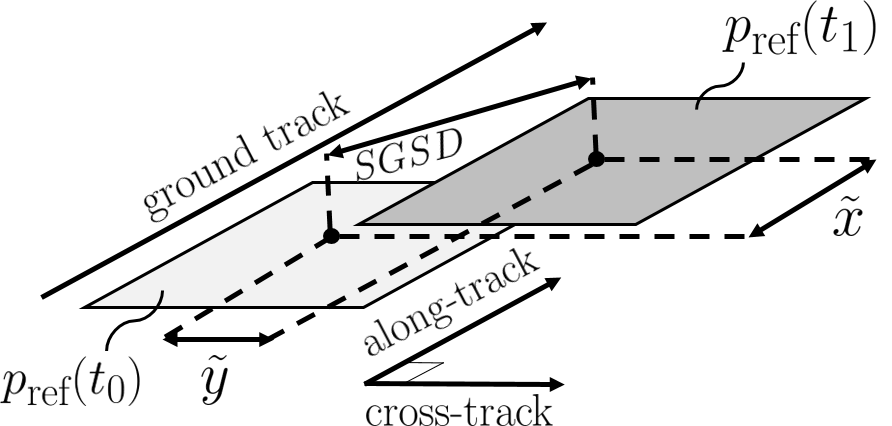
\includegraphics[width=70mm,angle=0]{figs/SGSD.png}
    \caption{Illustration of how SGSD is defined. $p_{\text{ref}}(t_1)$ and $p_{\text{ref}}(t_0)$ denote the reference pixel at time $t_1$ and $t_0$, respectively.} 
    \label{fig:SGSD}
\end{center}
\end{figure}
% The read-out distance, i.e. the distance covered between closing camera shutter and opening it again to capture the next frame, are defined in along-track and cross-track components as $v_{p,x}\delta t$ and $v_{p,y}\delta t$, respectively. In an ideal scenario for a pushbroom imager scanning uniformly in the along-track direction, the cross-track SGSD is zero, i.e. $\tilde{y}=0 \hspace{3pt} \rm{m}$ during $\Delta t = t_1-t_0$. 
Shown in Figure \ref{fig:SGSD}, the SGSD may therefore be defined as the distance between two sequential reference pixels during a camera integration time $\Delta t$, expressed by  along-track and cross-track components, as
\begin{subequations}
\begin{align}
    \tilde{x} & \triangleq v_{p,x}\Delta t, \label{eq:SGSD1} \\
    \tilde{y} & \triangleq v_{p,y}\Delta t. \label{eq:SGSD2}
\end{align}
\end{subequations}
The SGSD also determines the amount of overlap in the set of frames. If the scan direction is aligned with the velocity vector, and since the satellite has high speed as well as $\delta x$ being significantly larger than $\delta y$, it is preferred to slew about the $\hat{\mathbf{y}}_b$ axis to enable better along-track spatial resolution. From Eqs. (\ref{eq:rotational_vel1}) and (\ref{eq:rotational_vel2}) the required angular velocity of the satellite $\omega_{y}$ may be obtained from setting the desired SGSD and vice versa. Alternatively, $\omega_{y}$ and SGSD can be set if a a fixed target length shall be uniformly scanned. 
% if pitch angles at the start and at the end of image acquisition are equal in magnitude but of oppsite sign.
% The required angular velocities for selected integration times are shown in Figure \ref{fig:gsd_desired}.
% \begin{figure}[htbp]
%   \centering
%       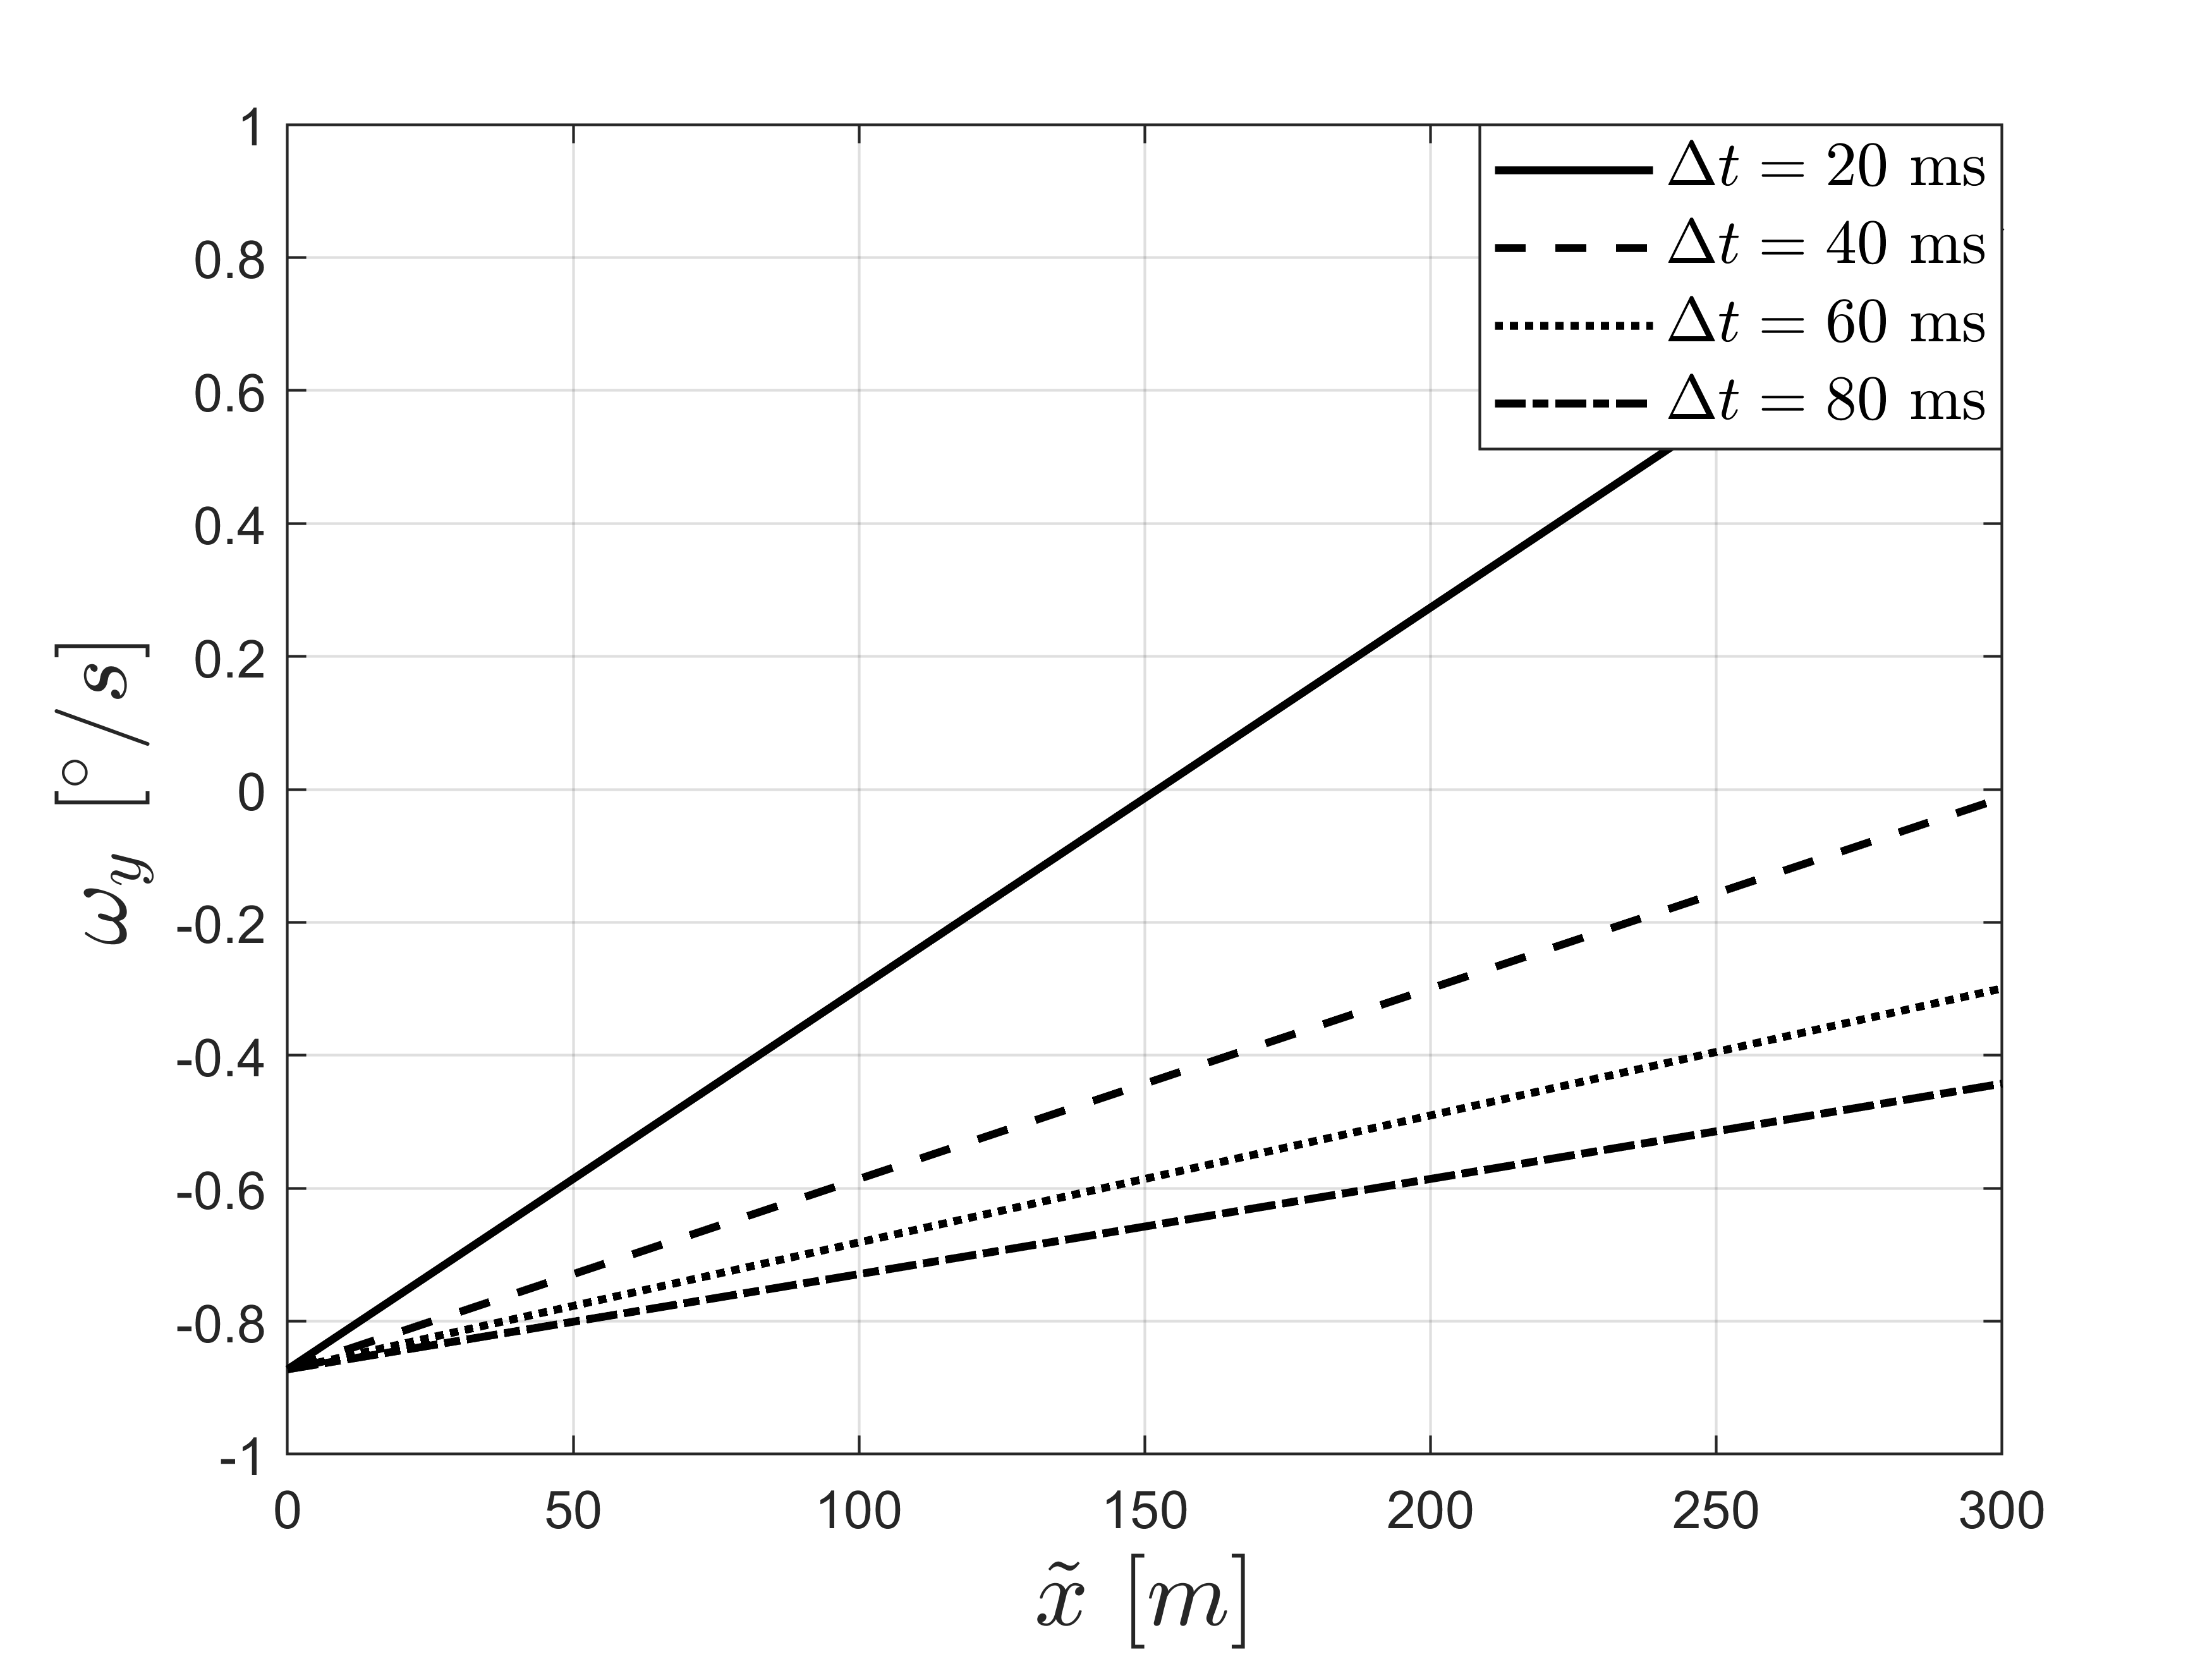
\includegraphics[width=0.48\textwidth]{figs/ang_vel_ref.png}
%   \caption{Reference angular rate $\dot{\theta}=\omega_{y}$ vs. desired along-track SGSD assuming $\omega_x=\omega_z=0$, for different integration times $\Delta t$. Altitude is $H=500 \hspace{3pt} \rm{km}$.}
% 	\label{fig:gsd_desired}
% \end{figure}
% \subsection{Slew Maneuver Strategies}
% \subsubsection{GSD-Driven Slew Maneuver}
% Suppose constant and small $\Delta t>0$, $\omega_{x}=\omega_{z}=0$, and $\psi=0$. Re-arranging Eqs. (\ref{eq:rotational_vel1}), the angular velocity of the satellite may be chosen from desired instantaneous in-track GSD $\tilde{x}_{\text{ref}}$ as
% \begin{align}
% \dot{\theta}_{\text{ref}} &= \frac{1}{H}\Big(v_{s}-v_{g,x}+\frac{\tilde{x}_{\text{ref}}}{\Delta t}\Big). \label{eq:desired_inst_gsd_x}
% \end{align}
\subsection{Imaging Strategy} 
Consider the length $s_{g}$ that shall be observed during the time $\Delta T=t_f-t_0$ and the satellite rotating from start to end pitch angles $\theta(t_0)=\theta_0$ and $\theta(t_f)=\theta_f$. Assuming constant altitude, to uniformly scan the target the final pitch angle may be set to $\theta_f=-\theta_0$ such that $\delta x(t_0)=\delta x (t_f)$. The geometry is shown in Figure \ref{fig:orbit-track}. Furthermore, it is assumed that $\omega_{z} = \omega_{x} = 0$, $\phi=\psi=0$ such that $\omega_y=\dot{\theta}$. 
\begin{figure}[htbp]
  \centering
      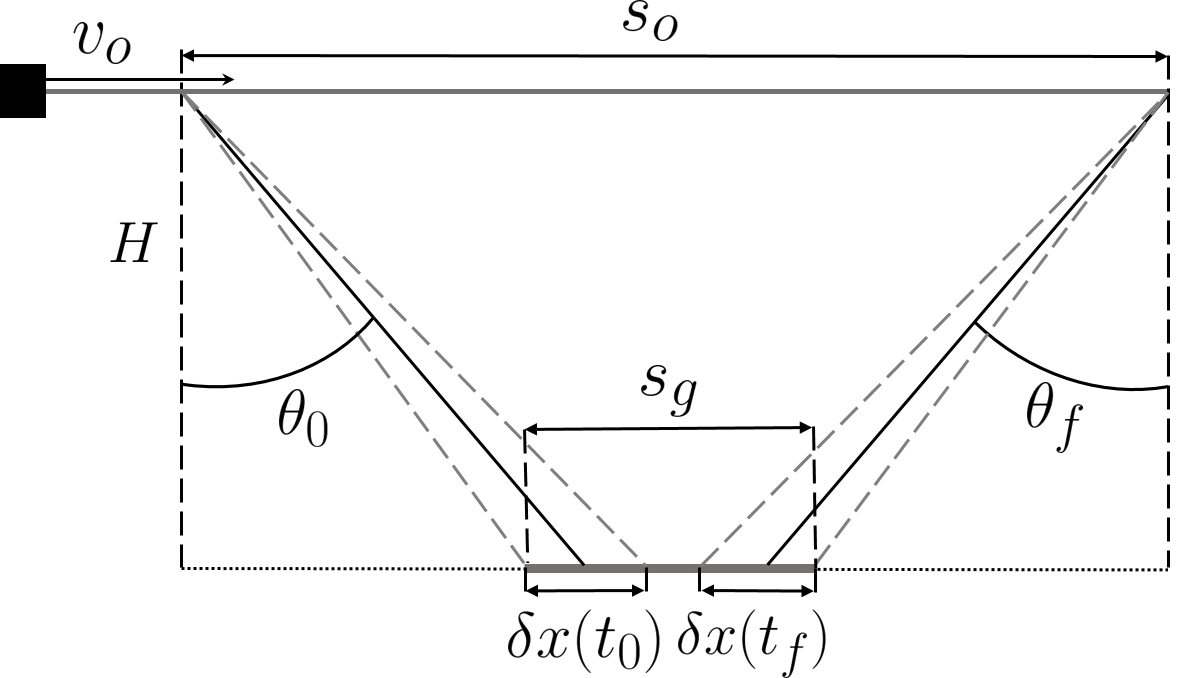
\includegraphics[width=0.45\textwidth]{figs/orbit_track.png}
  \caption{Geometry of a satellite slewing across a ground target with objective to acquire images along the distance $s_g$. Altitude is $H=500 \hspace{3pt} \rm{km}$.}
	\label{fig:orbit-track}
\end{figure}
The orbit track can be calculated as
\begin{align}
s_{o}&=s_{g}+H\Bigg(\tan\bigg(\theta_0-\frac{\epsilon_{w}}{2}\bigg)-\tan\bigg(\theta_f-\frac{\epsilon_{w}}{2}\bigg)\Bigg).
\end{align}
The time $\Delta T$ required to perform the slew maneuver, can be calculated as
\begin{align}
\Delta T & = \frac{s_{o}}{v_{o}},
\end{align}
and the angular velocity of the spacecraft may found from
\begin{equation}
\omega_{y}=\dot{\theta} = \frac{\Delta \theta}{\Delta T}.
\end{equation}
Figure \ref{fig:slew_angle} shows required angular velocity $\omega_y$ as a function of $\theta_0=-\theta_f$ for varying length $s_g$ to be observed.
\begin{figure}[htbp]
  \centering
      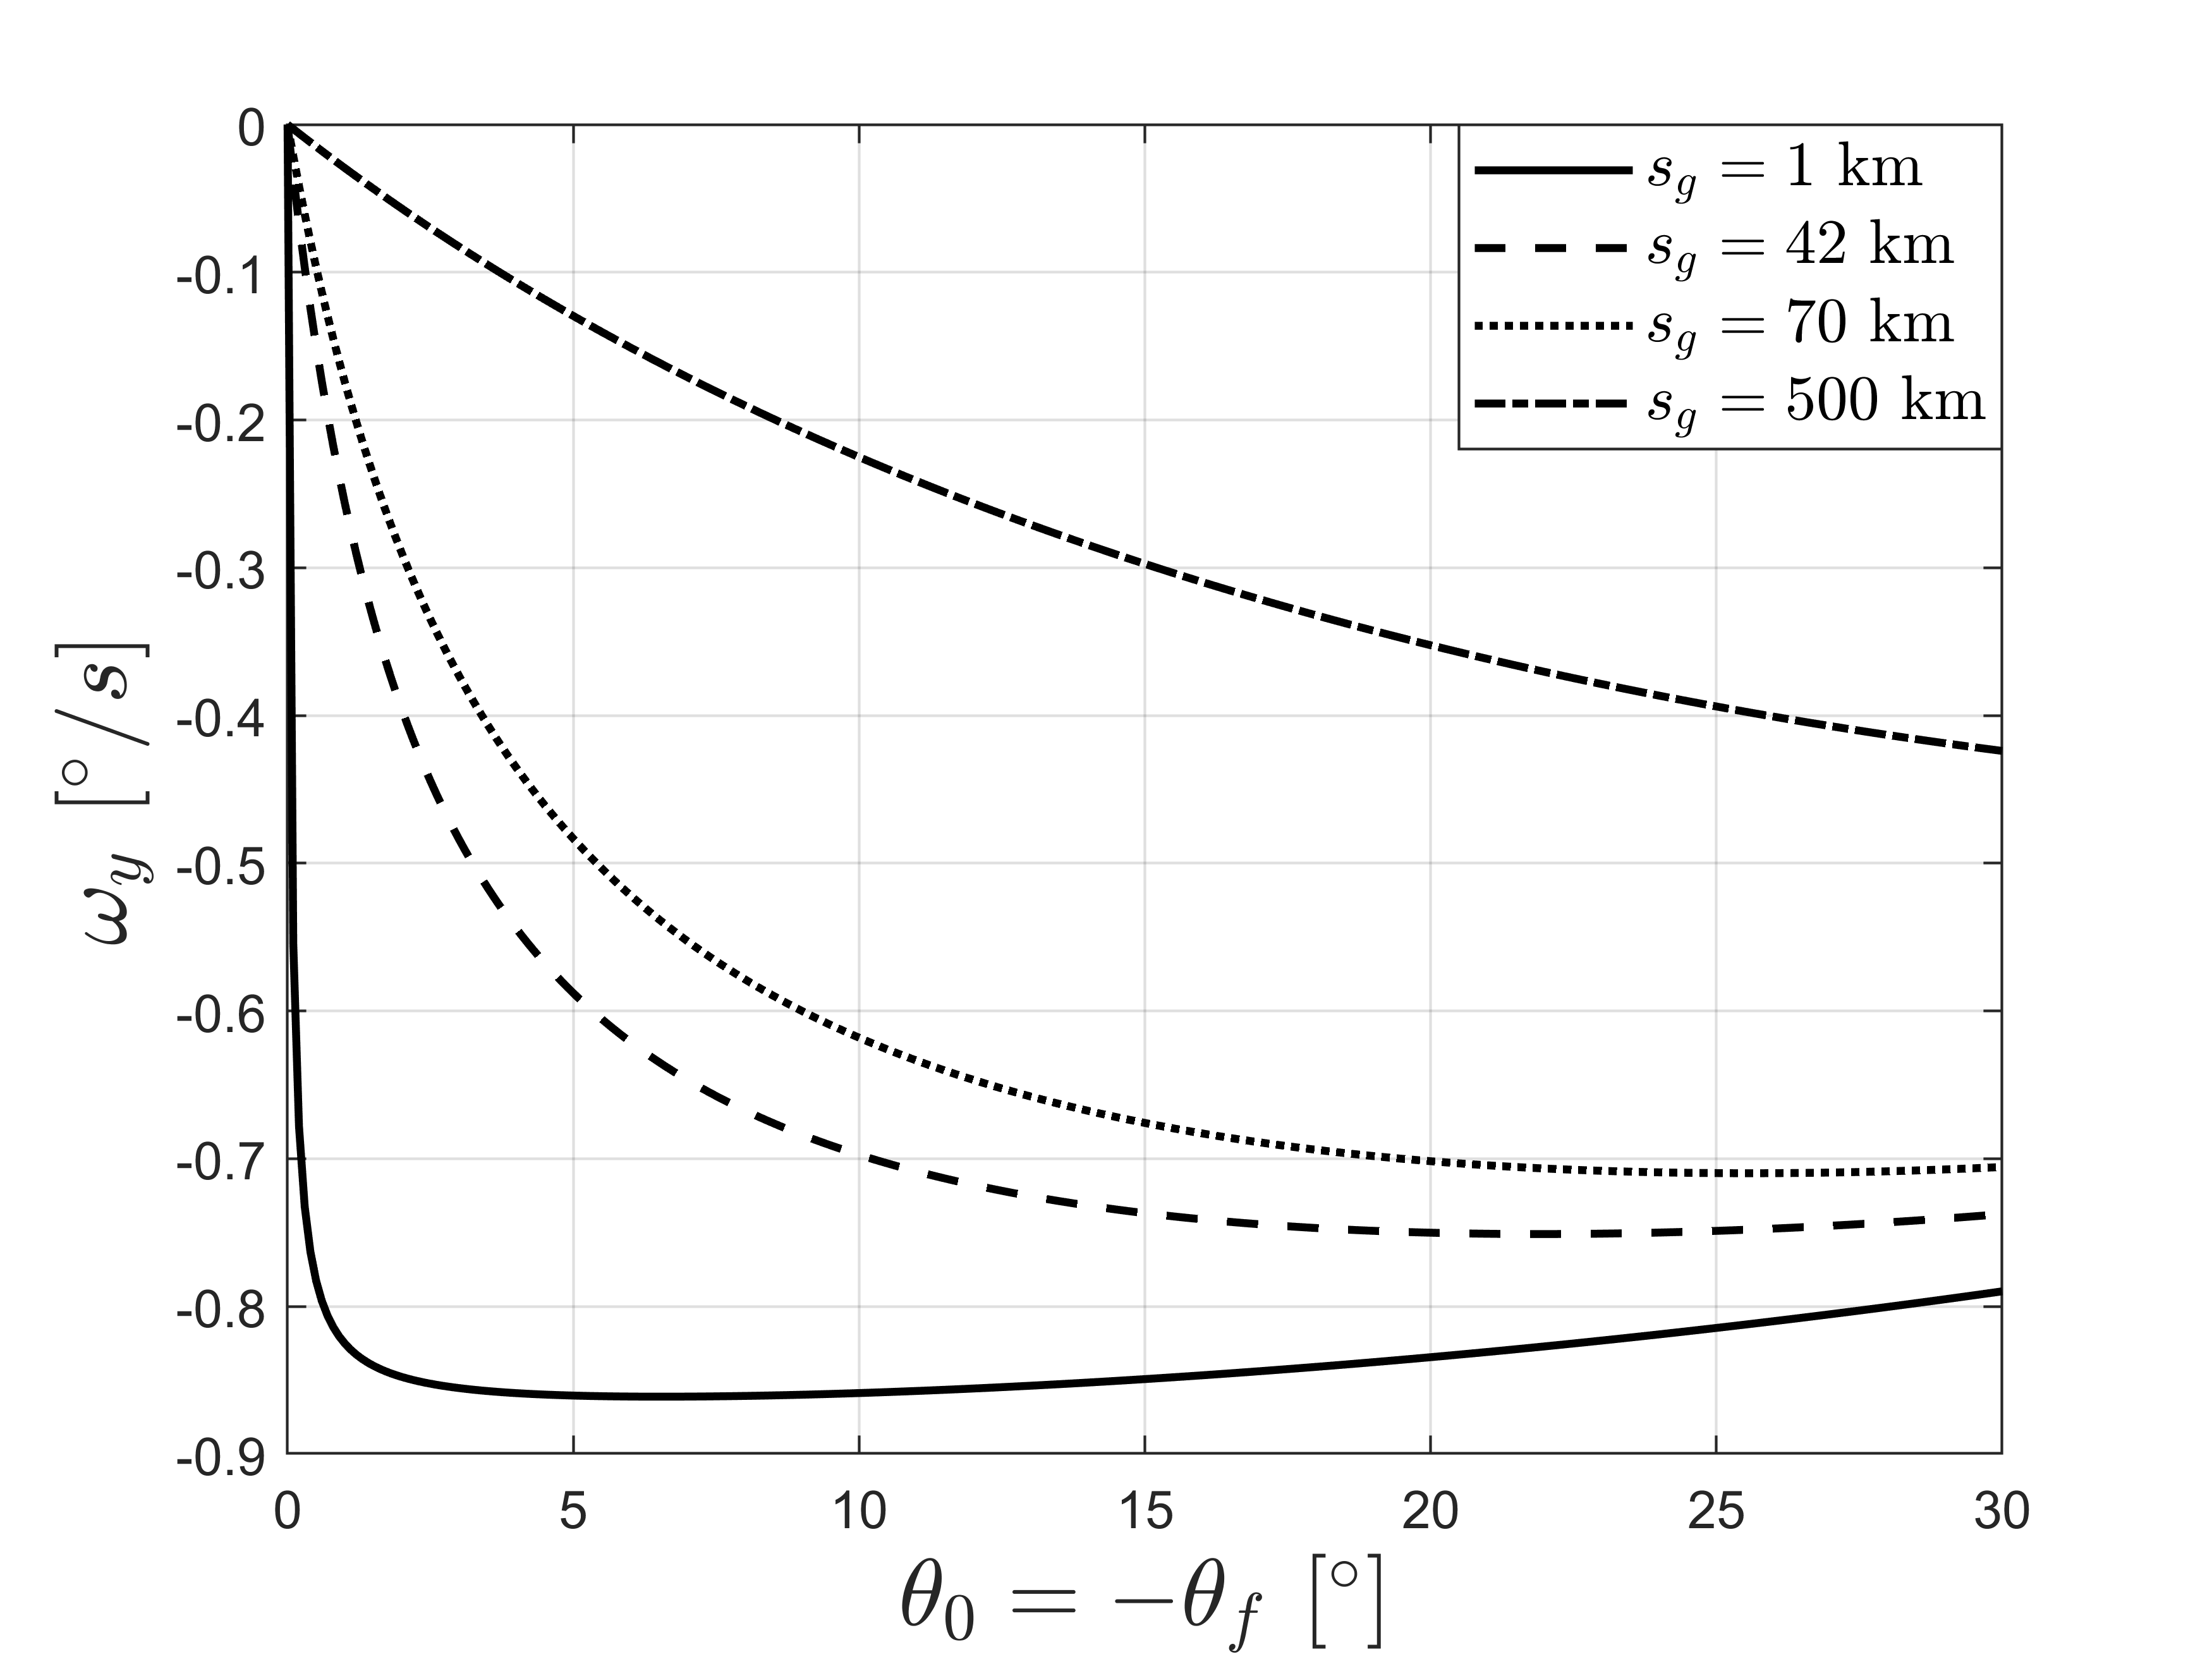
\includegraphics[width=0.48\textwidth]{figs/ang_vel_track.png}
  \caption{Angular velocity $\omega_{y}$ vs. pitch angles $\theta_0=-\theta_f$ for different $s_g$. Altitude is $H=500 \hspace{3pt} \rm{km}$.}
	\label{fig:slew_angle}
\end{figure}
\subsection{Expected Performance}
\subsubsection{Resolution for Nadir-pointing} \label{sec:spacecraft_nadir} 
\begin{table}[htbp]
	\caption{Simulation parameters}
	\label{tab:camera_params}
	\centering
			\begin{tabular}{l r}
				\hline
                Parameter & Value \\
                \hline
                FPS & 22 \\ 
                Camera Integration time $\Delta t$ & $45.4 \hspace{3pt} \rm{ms}$ \\
                Camera Exposure time $\tau$ & $41.4 \hspace{3pt} \rm{ms}$ \\
                Camera Read-out time $\delta t$ & $4 \hspace{3pt} \rm{ms}$ \\
                Target length $s_g$ & $40.08 \hspace{3pt} \rm{km}$ \\
                Altitude $H$ & $500 \hspace{3pt} \rm{km}$ \\
                Satellite speed $v_o$ & $7.61 \hspace{3pt} \rm{km/s}$ \\
                Roll angle $\phi$ & $0^{\circ}$ \\
                Yaw angle $\psi$ & $0^{\circ}$ \\
				\hline
				\end{tabular}
\end{table}
With hyperspectral imager's scan direction being aligned with the along-track direction while pointing at nadir, i.e. $\theta=0^{\circ}$, its instantaneous pixel resolution is $\delta x =500 \hspace{3pt} \rm{m}$. Using the specifications in Table \ref{tab:optics} and camera settings in Table \ref{tab:camera_params}, the obtained spatial resolution is $\Delta x = 815.6 \hspace{3pt} \rm{m}$, $\Delta y =58.6 \hspace{3pt} \rm{m}$ and a swath width of $P_{h}=40.08 \hspace{3pt} \rm{km}$. The along-track SGSD becomes $\tilde{x} =346 \hspace{3pt} \rm{m}$, meaning that $3$ frames partially overlap. It takes $\Delta T = 5.23 \hspace{3pt} \rm{s}$ to scan a target length of $s_g=s_o=40.08 \hspace{3pt} \rm{km}$.
\subsubsection{Resolution for Slew Maneuver} \label{sec:spacecraft_slew}
Using the same parameters in Tables \ref{tab:optics} and \ref{tab:camera_params} are used for imaging during a slew maneuver, Figures \ref{fig:spatial_time} and \ref{fig:cross_spatial_time} show how spatial resolution varies with different pitch rates in ideal settings where no attitude errors are present. Table \ref{tab:SGSD} shows the corresponding SGSD, reference angular velocity and duration for each starting pitch angle $\theta_0$. For example with $\theta_0=20^{\circ}$ as starting pitch angle, the satellite would have to slew at a reference angular velocity of $\omega_{y}= -0.754^{\circ}/\rm{s}$ for $\Delta T = 53.05 \hspace{3pt} \rm{s}$ to cover the target length $s_g=40.08 \hspace{3pt} \rm{km}$ uniformly. The spatial resolution varies between $\Delta x=609.2 \hspace{3pt} \rm{m}$ at $\theta=20^{\circ}$ to $\Delta x= 542.9 \hspace{3pt} \rm{m}$ at $\theta=0^{\circ}$. Additionally, a SGSD of $\tilde{x} = 47.09 \hspace{3pt} \rm{m}$ is achieved instead of $\tilde{x} = 346 \hspace{3pt} \rm{m}$ for the nadir-pointing case. This means there will be at least $12$ frames that partially overlap in the along-track direction, instead of $3$ for nadir-pointing. 

In reality, due to attitude stabilization inaccuracies and system noise, the spatial resolution and SGSD will vary significantly throughout the image acquisition. With reference to the image resolution requirement discussed in Section \ref{sec:mission-design}, in order to have a sequential pixel-to-pixel distance to be less than $100 \hspace{3pt} \rm{m}$, by using Eqs. \ref{eq:fov_x} and \ref{eq:footprint_x}, the attitude error requirement is
\begin{align}
    \vert \delta \theta \vert &< \arctan\bigg(\frac{\vert100-\tilde{x}\vert}{H\sec(\phi+\delta\phi)}+\tan(\theta) \bigg)-\theta, \label{eq:attitude_error}
\end{align}
\noindent which indicates a precise ADCS is required. Figure \ref{fig:dtheta} shows how the required attitude accuracy varies throughout the slew maneuvers with different SGSD.
% For example, even in the best case when SGSD shall be exactly zero at nadir, i.e. $\tilde{x}=0 \hspace{3pt} \rm{m}$ and $\theta=0^{\circ}$, then better than $\pm 0.011^{\circ}$ attitude accuracy is needed. 
With a desired SGSD of $\tilde{x}=47.09 \hspace{3pt} \rm{m}$ at $\theta=20^{\circ}$ and $\phi=0^{\circ}$, using Eq. (\ref{eq:attitude_error}) and assuming $\sec(\phi+\delta\phi)\approx 1$, the attitude accuracy of  $\vert\delta \theta\vert<\pm 0.00535^{\circ}$ is required. For $\theta=10^{\circ}$ and $\tilde{x}=66.96\hspace{3pt} \rm{m}$ then $\vert\delta \theta\vert\pm 0.003672^{\circ}$ is required while for $\theta=30^{\circ}$ and $\tilde{x}=52.59\hspace{3pt} \rm{m}$ then $\vert\delta \theta\vert<0.004075^{\circ}$ is required.
  


% \begin{figure}[htbp]
%   \centering
%       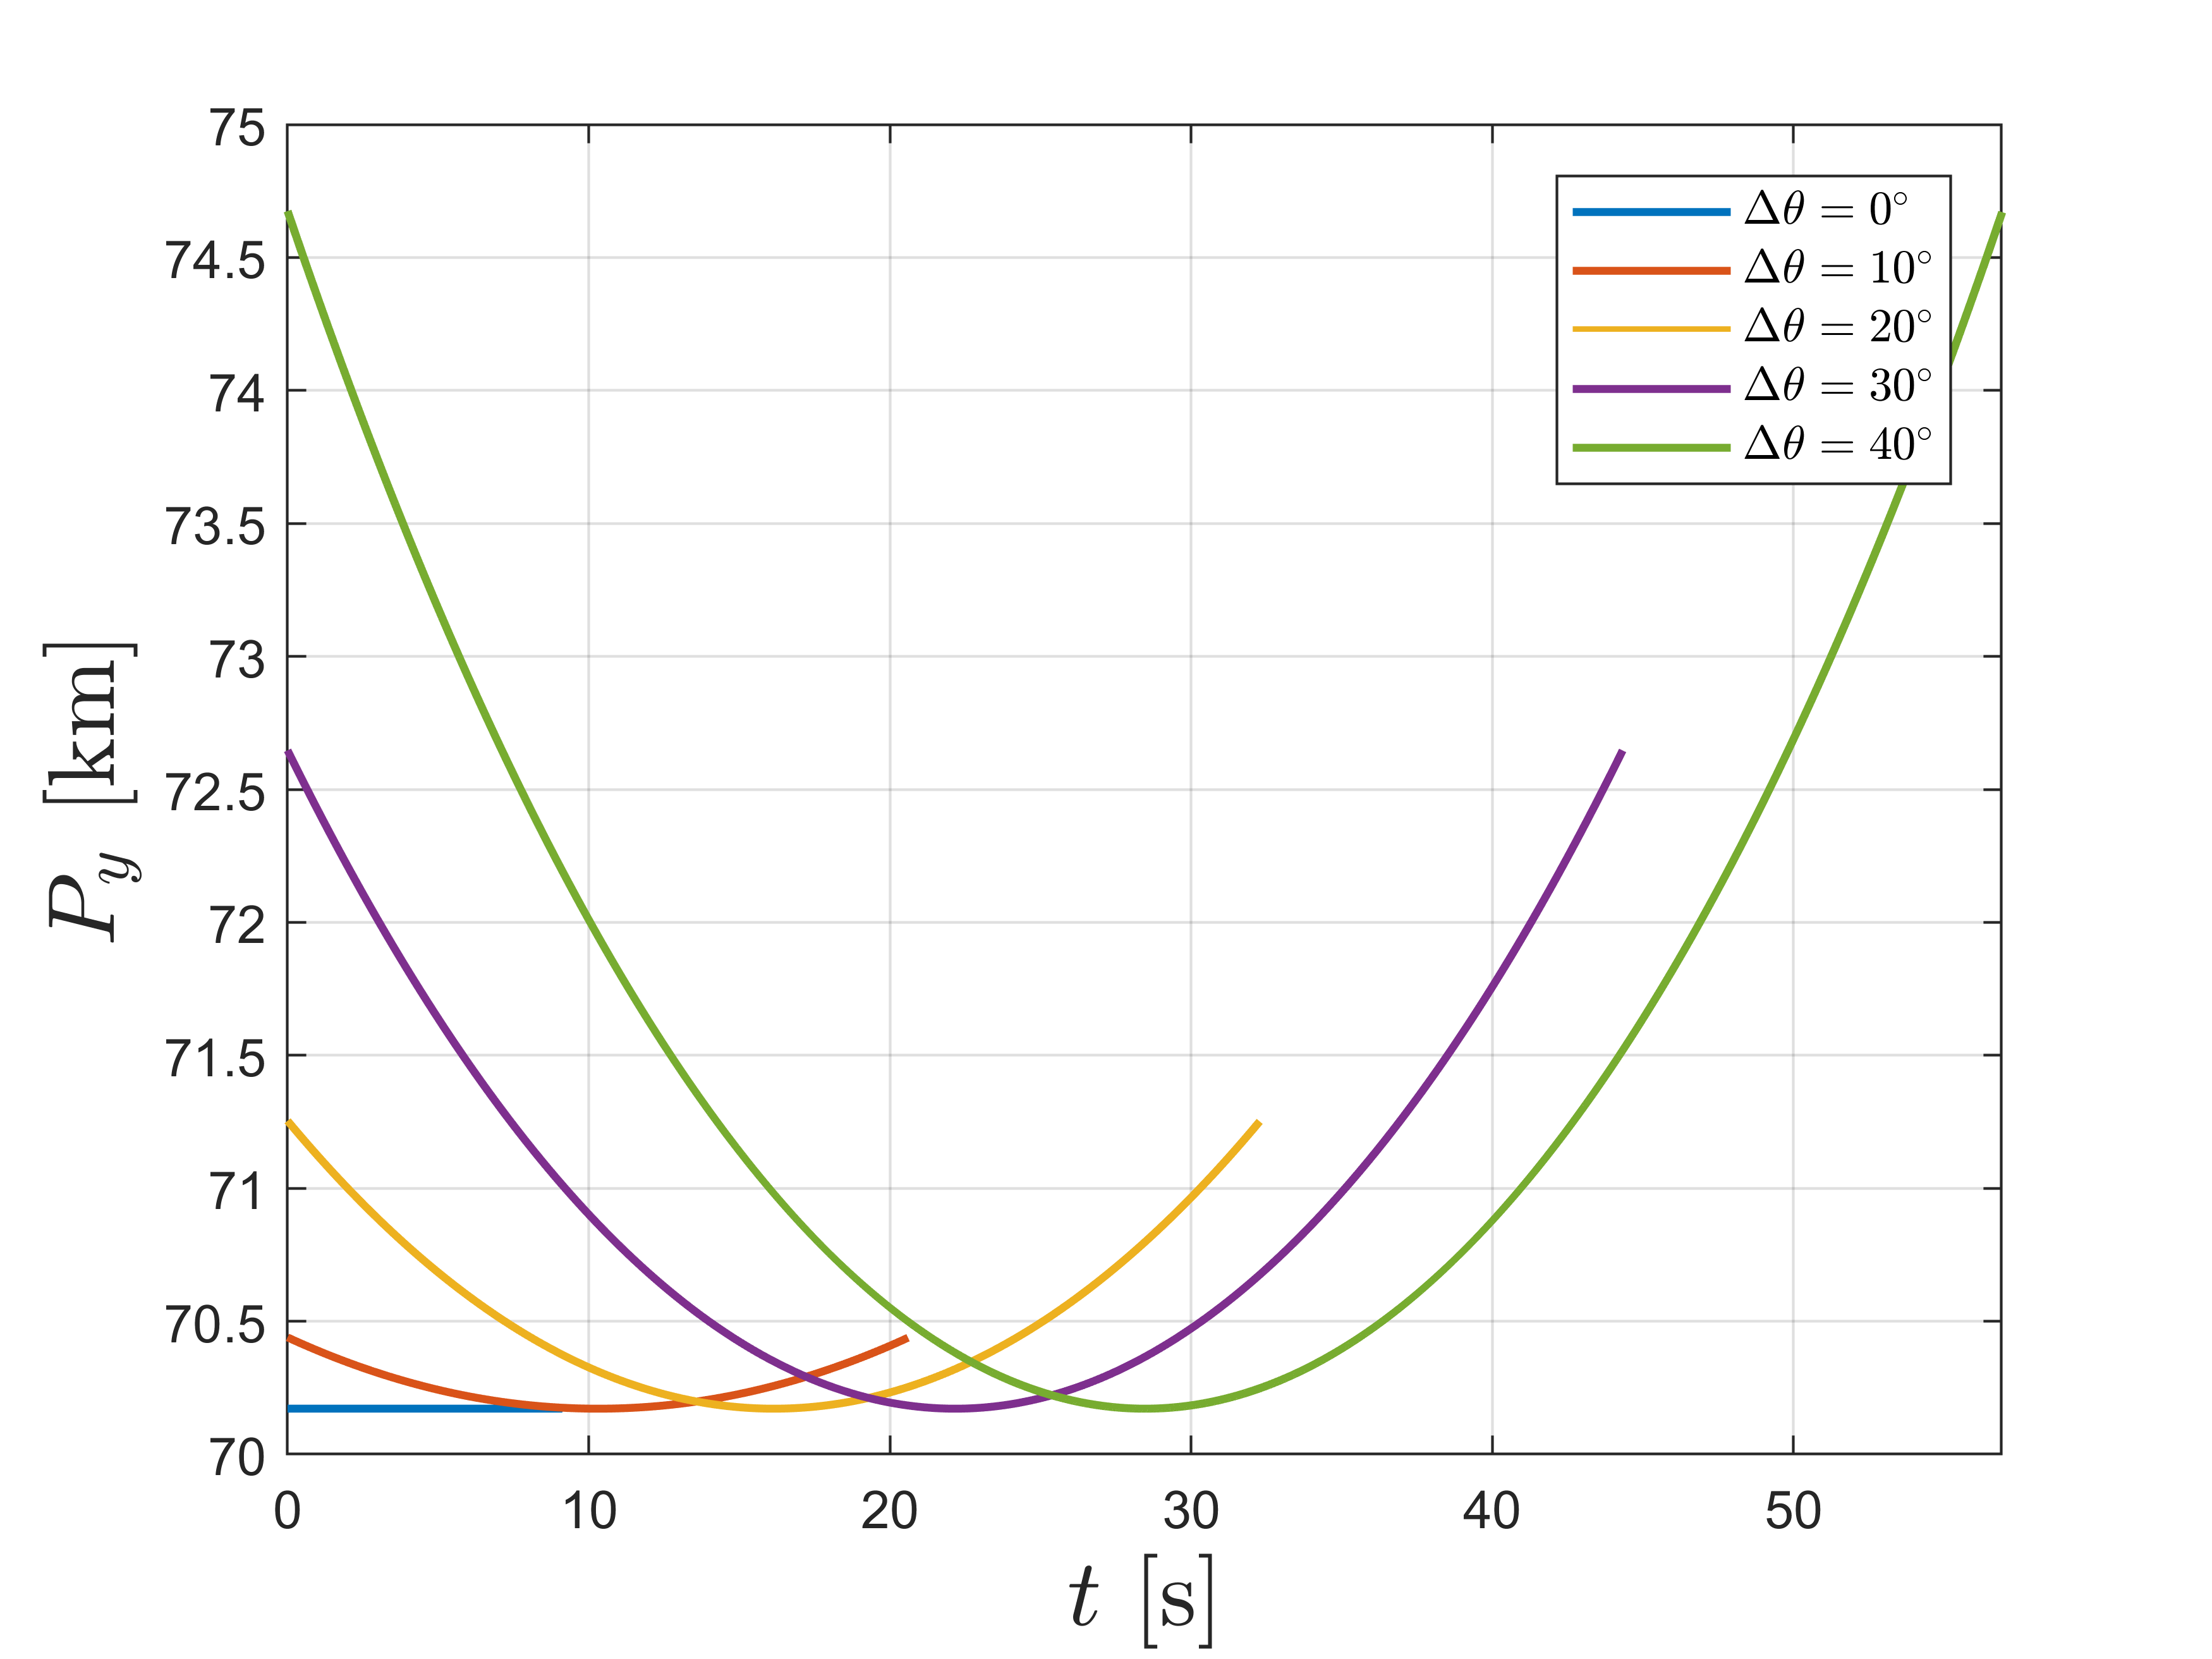
\includegraphics[width=0.45\textwidth]{figs/swath_time.png}
%   \caption{Swath width for different starting/ending pitch angles $\theta(T_0)=-\theta(T_f)$ and angular velocities $\omega_{y}$. Target track is $s_g=70 \hspace{3pt} \rm{km}$.}
% 	\label{fig:swath_time}
% \end{figure}
\begin{figure}[htbp]
  \centering
      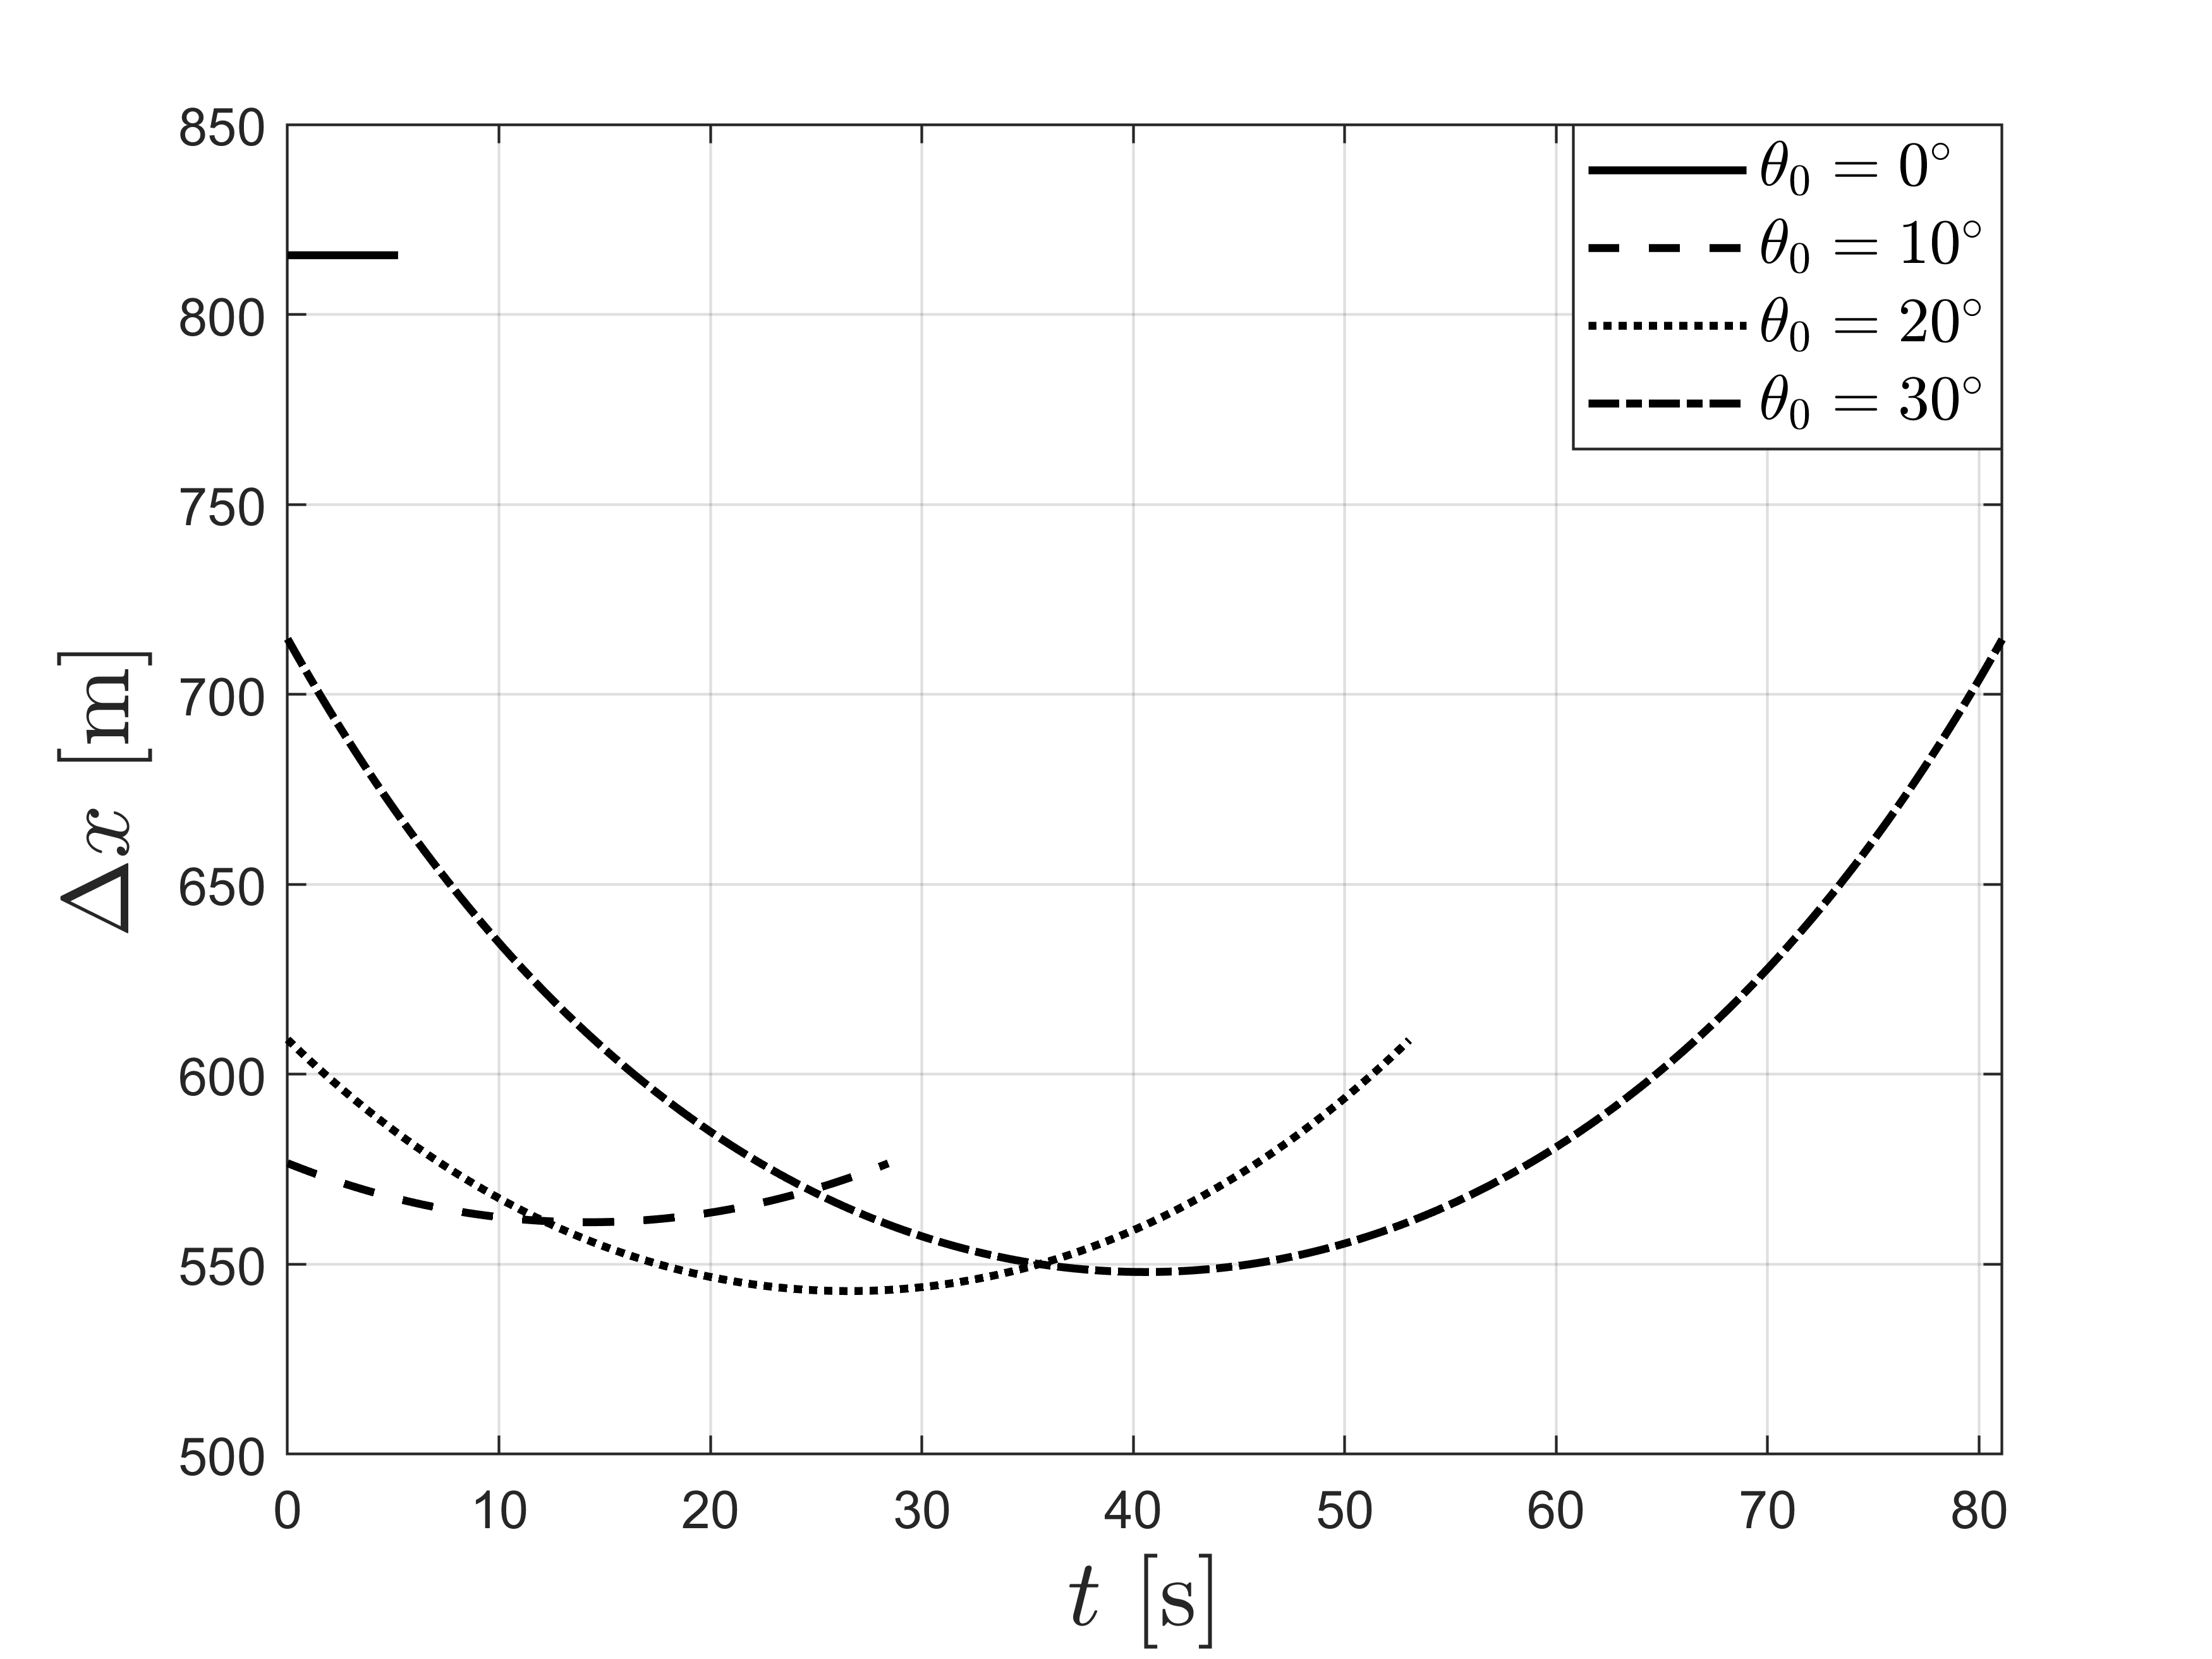
\includegraphics[width=0.48\textwidth]{figs/Delta_x.png}
  \caption{Along-track spatial resolution for different pitch angles $\theta_0=-\theta_f$ and angular velocities $\omega_{y}$.}
	\label{fig:spatial_time}
\end{figure}
\begin{figure}[htbp]
  \centering
      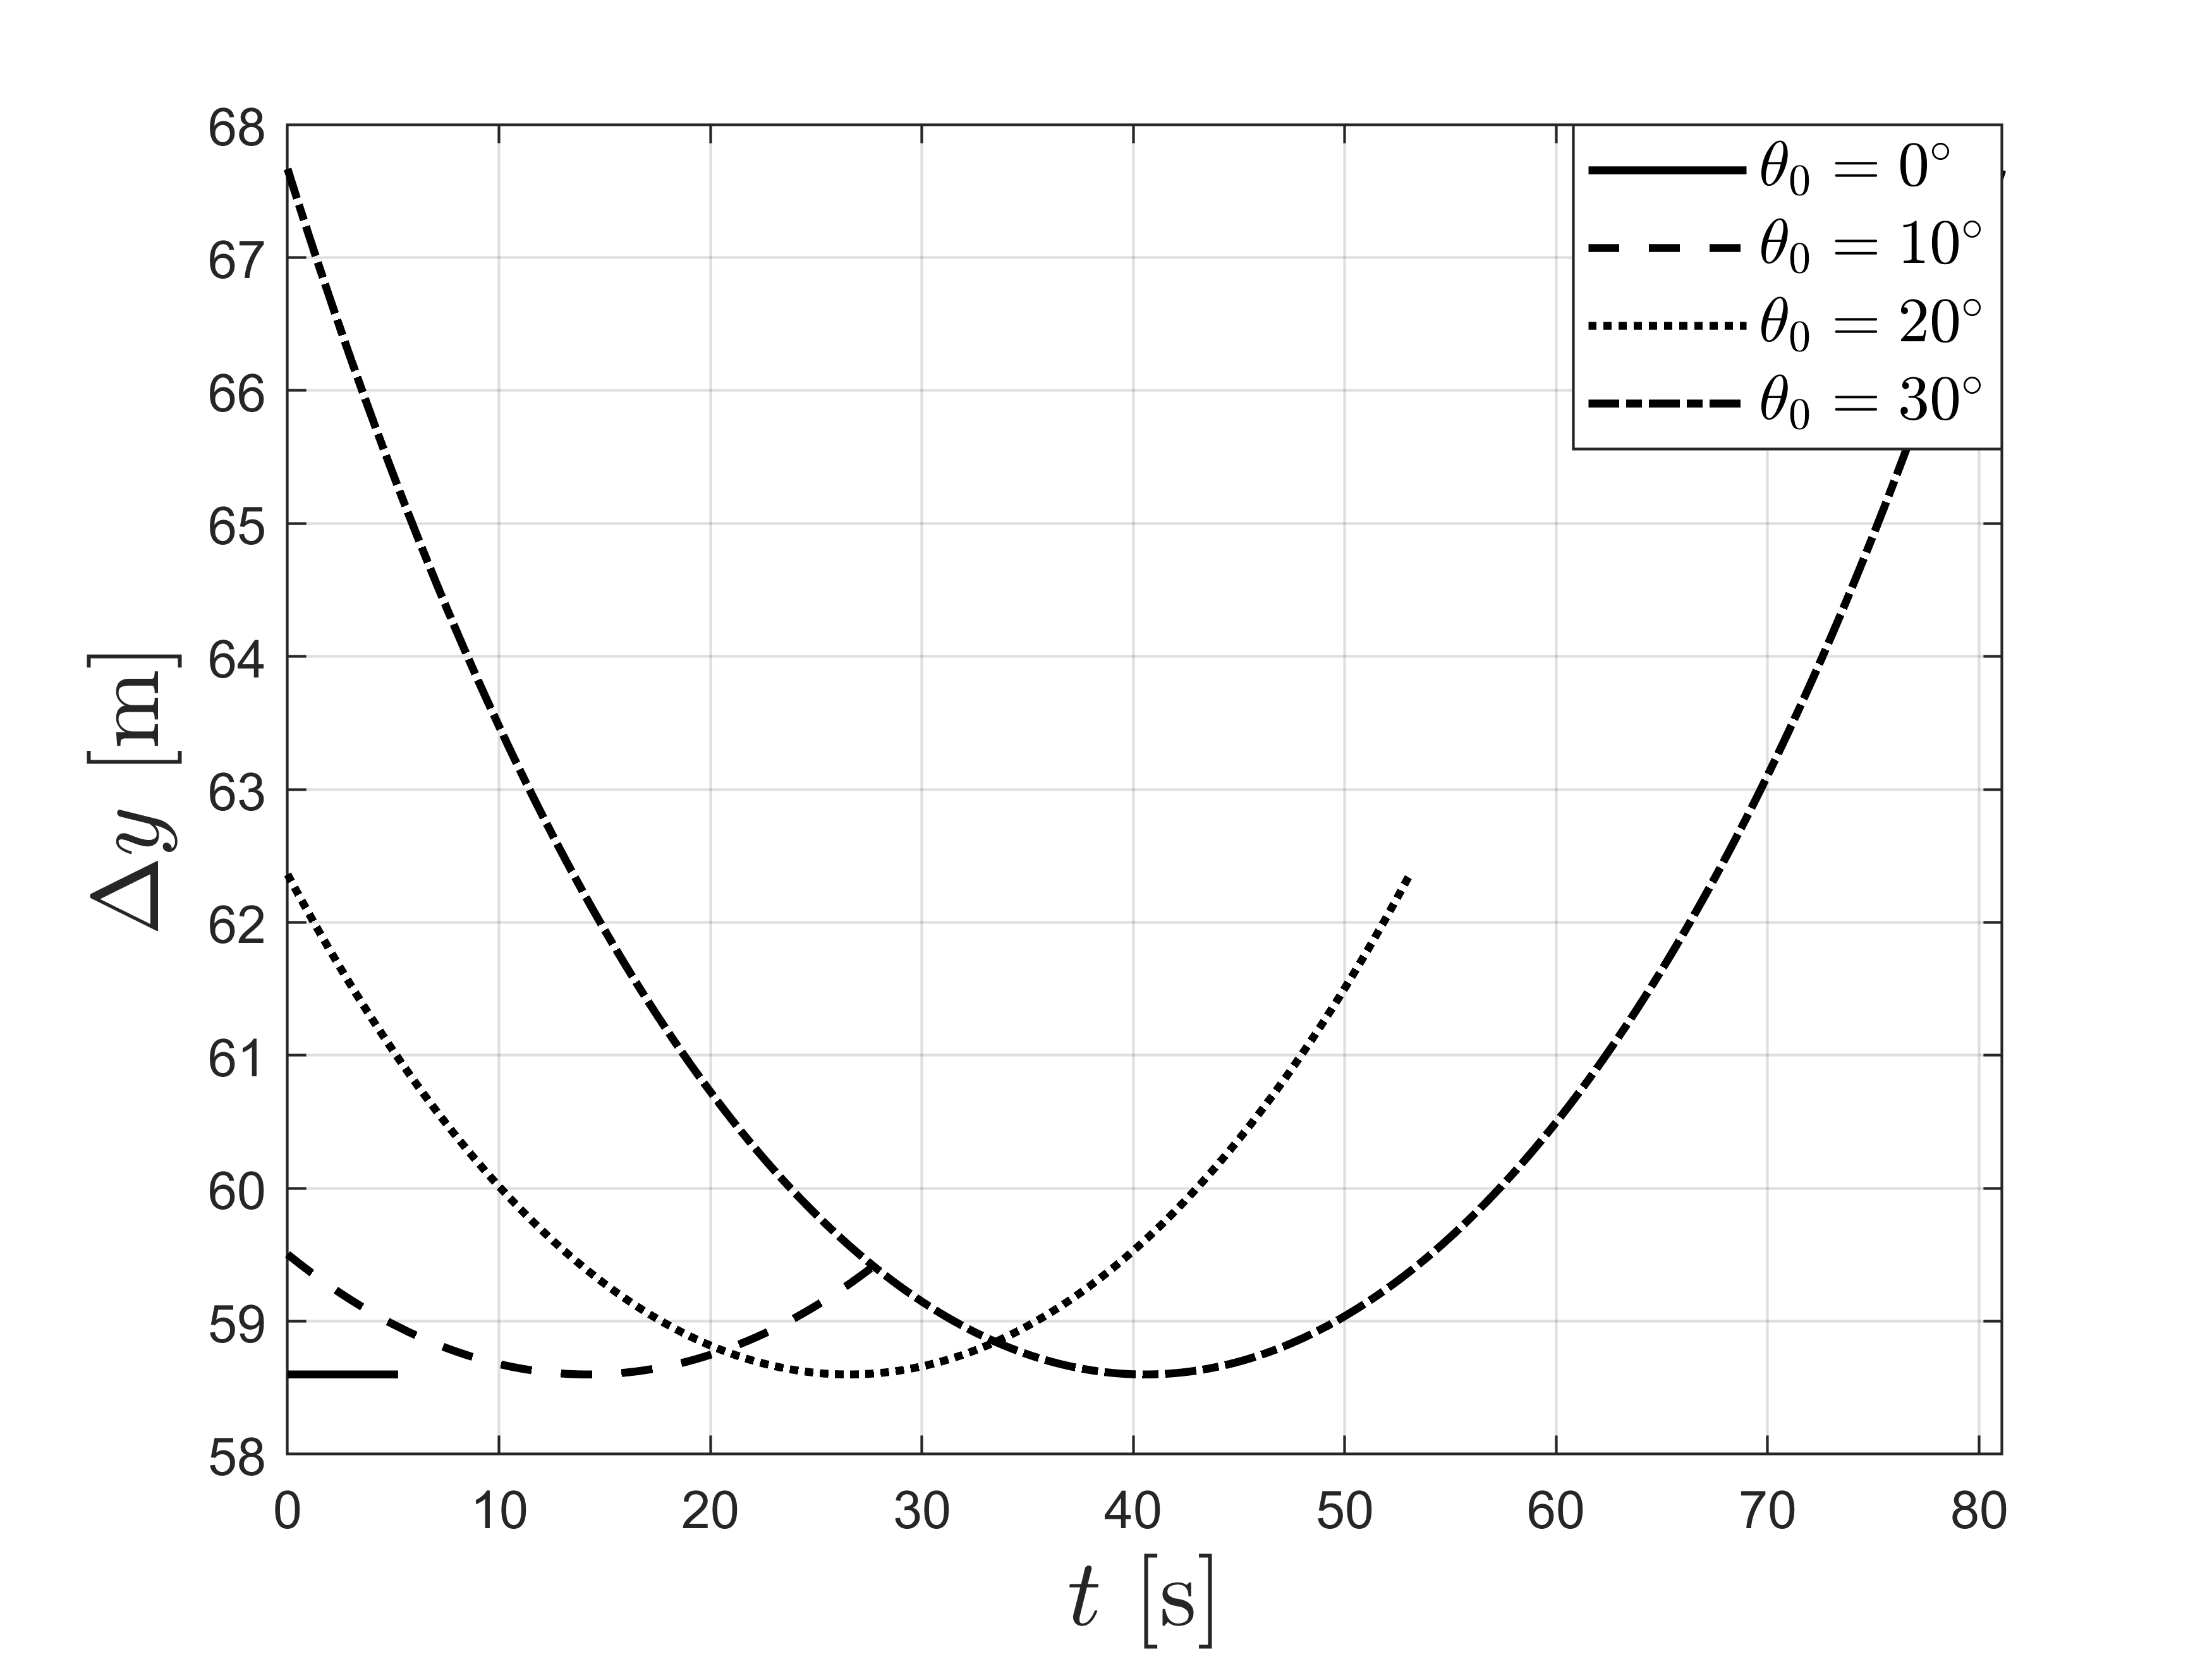
\includegraphics[width=0.48\textwidth]{figs/Delta_y.png}
  \caption{Cross-track spatial resolution for different pitch angles $\theta_0=-\theta_f$ and angular velocities $\omega_{y}$.}
	\label{fig:cross_spatial_time}
\end{figure}
% \begin{figure}[htbp]
%   \centering
%       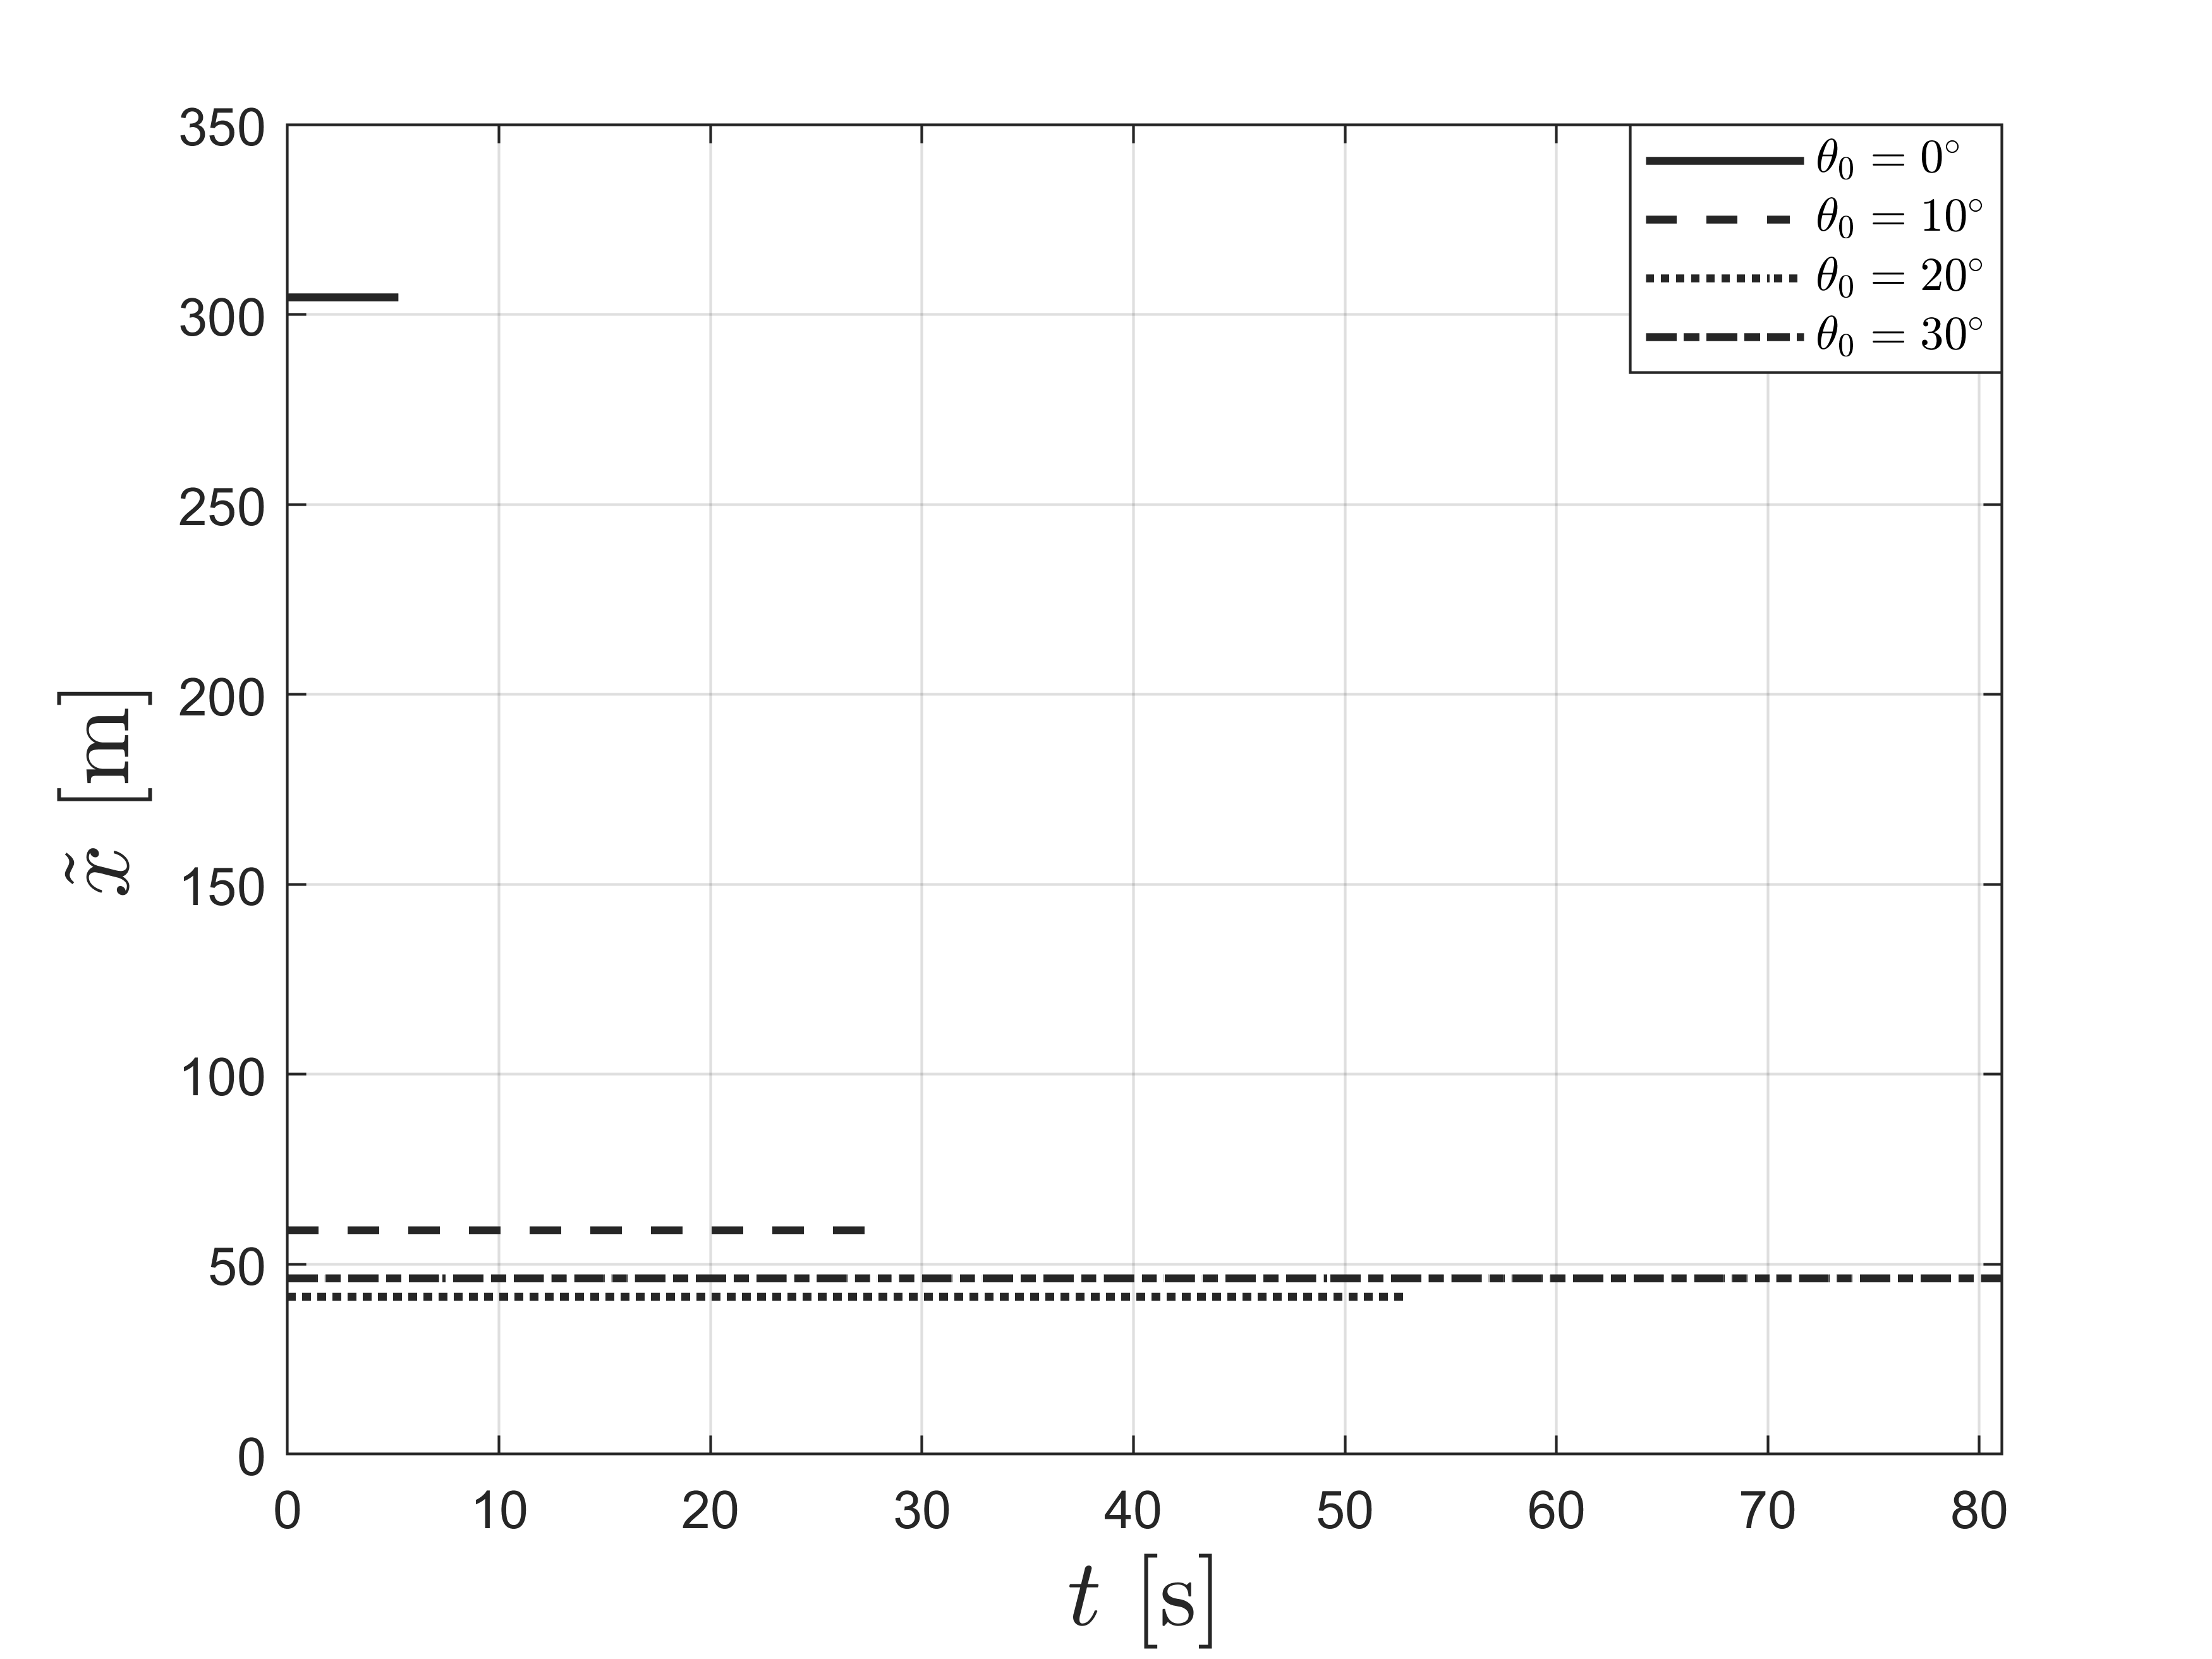
\includegraphics[width=0.48\textwidth]{figs/GSD_x.png}
%   \caption{Along-track SGSD for different starting/ending pitch angles $\theta_0=-\theta_f$ and angular velocities $\omega_{y}$. Target track is $s_g=42.41 \hspace{3pt} \rm{km}$.\hl{tabulate}}
% 	\label{fig:GSDx}
% \end{figure}
\begin{table}[htbp]
	\caption{Along-track SGSD}
	\label{tab:SGSD}
	\centering
			\begin{tabular}{l l l| l}
				\hline
				$\theta_0$ [$^{\circ}$] & $\omega_y$ [$^{\circ}\rm{/s}$] & $\Delta T$ [$\rm{s}$]&  $\tilde{x}$ [$\rm{m}$] \\
				\hline
				0 & 0 & 5.23 & 346  \\
				10 & -0.704 & 28.41 & 66.96 \\
				20 & -0.754 & 53.05 & 47.09 \\
				30 & -0.740 & 81.09 & 52.59 \\
				\hline
				\end{tabular}
\end{table}
\begin{figure}[htbp]
  \centering
      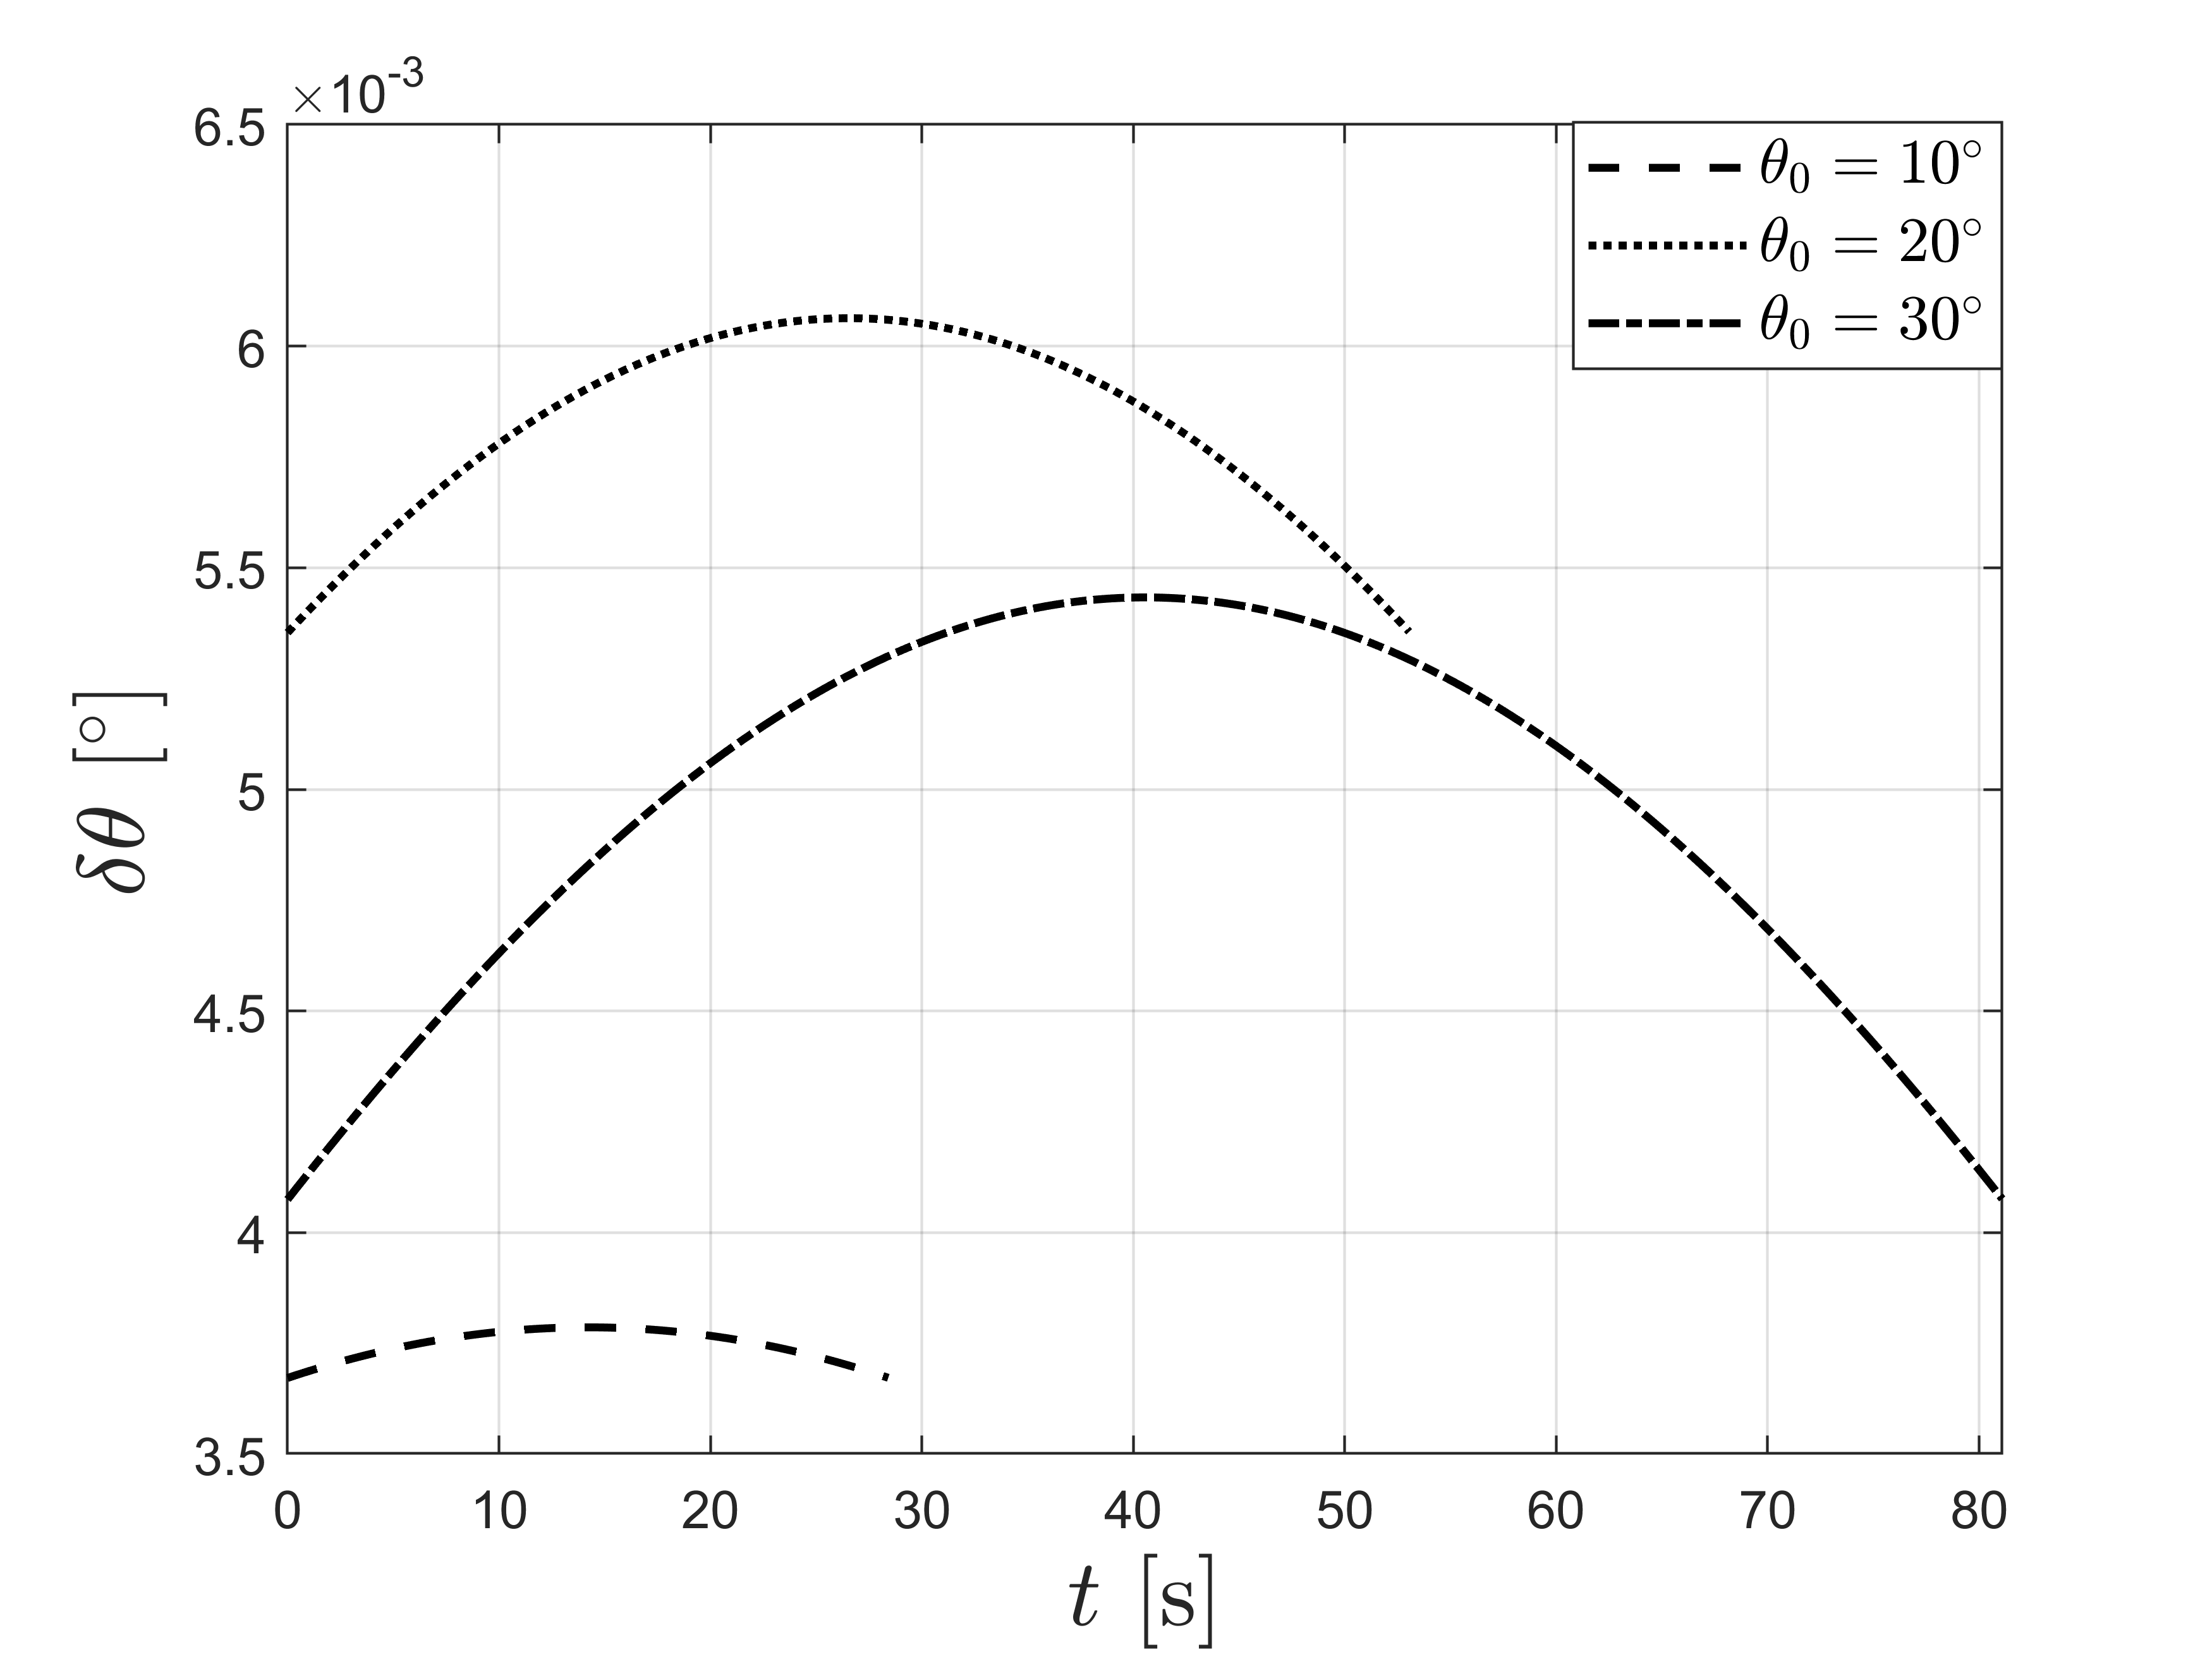
\includegraphics[width=0.48\textwidth]{figs/dtheta.png}
  \caption{Required pitch accuracy throughout the slew maneuvers for different $\theta_0$.}
	\label{fig:dtheta}
\end{figure}
% \begin{figure}[htbp]
%   \centering
%       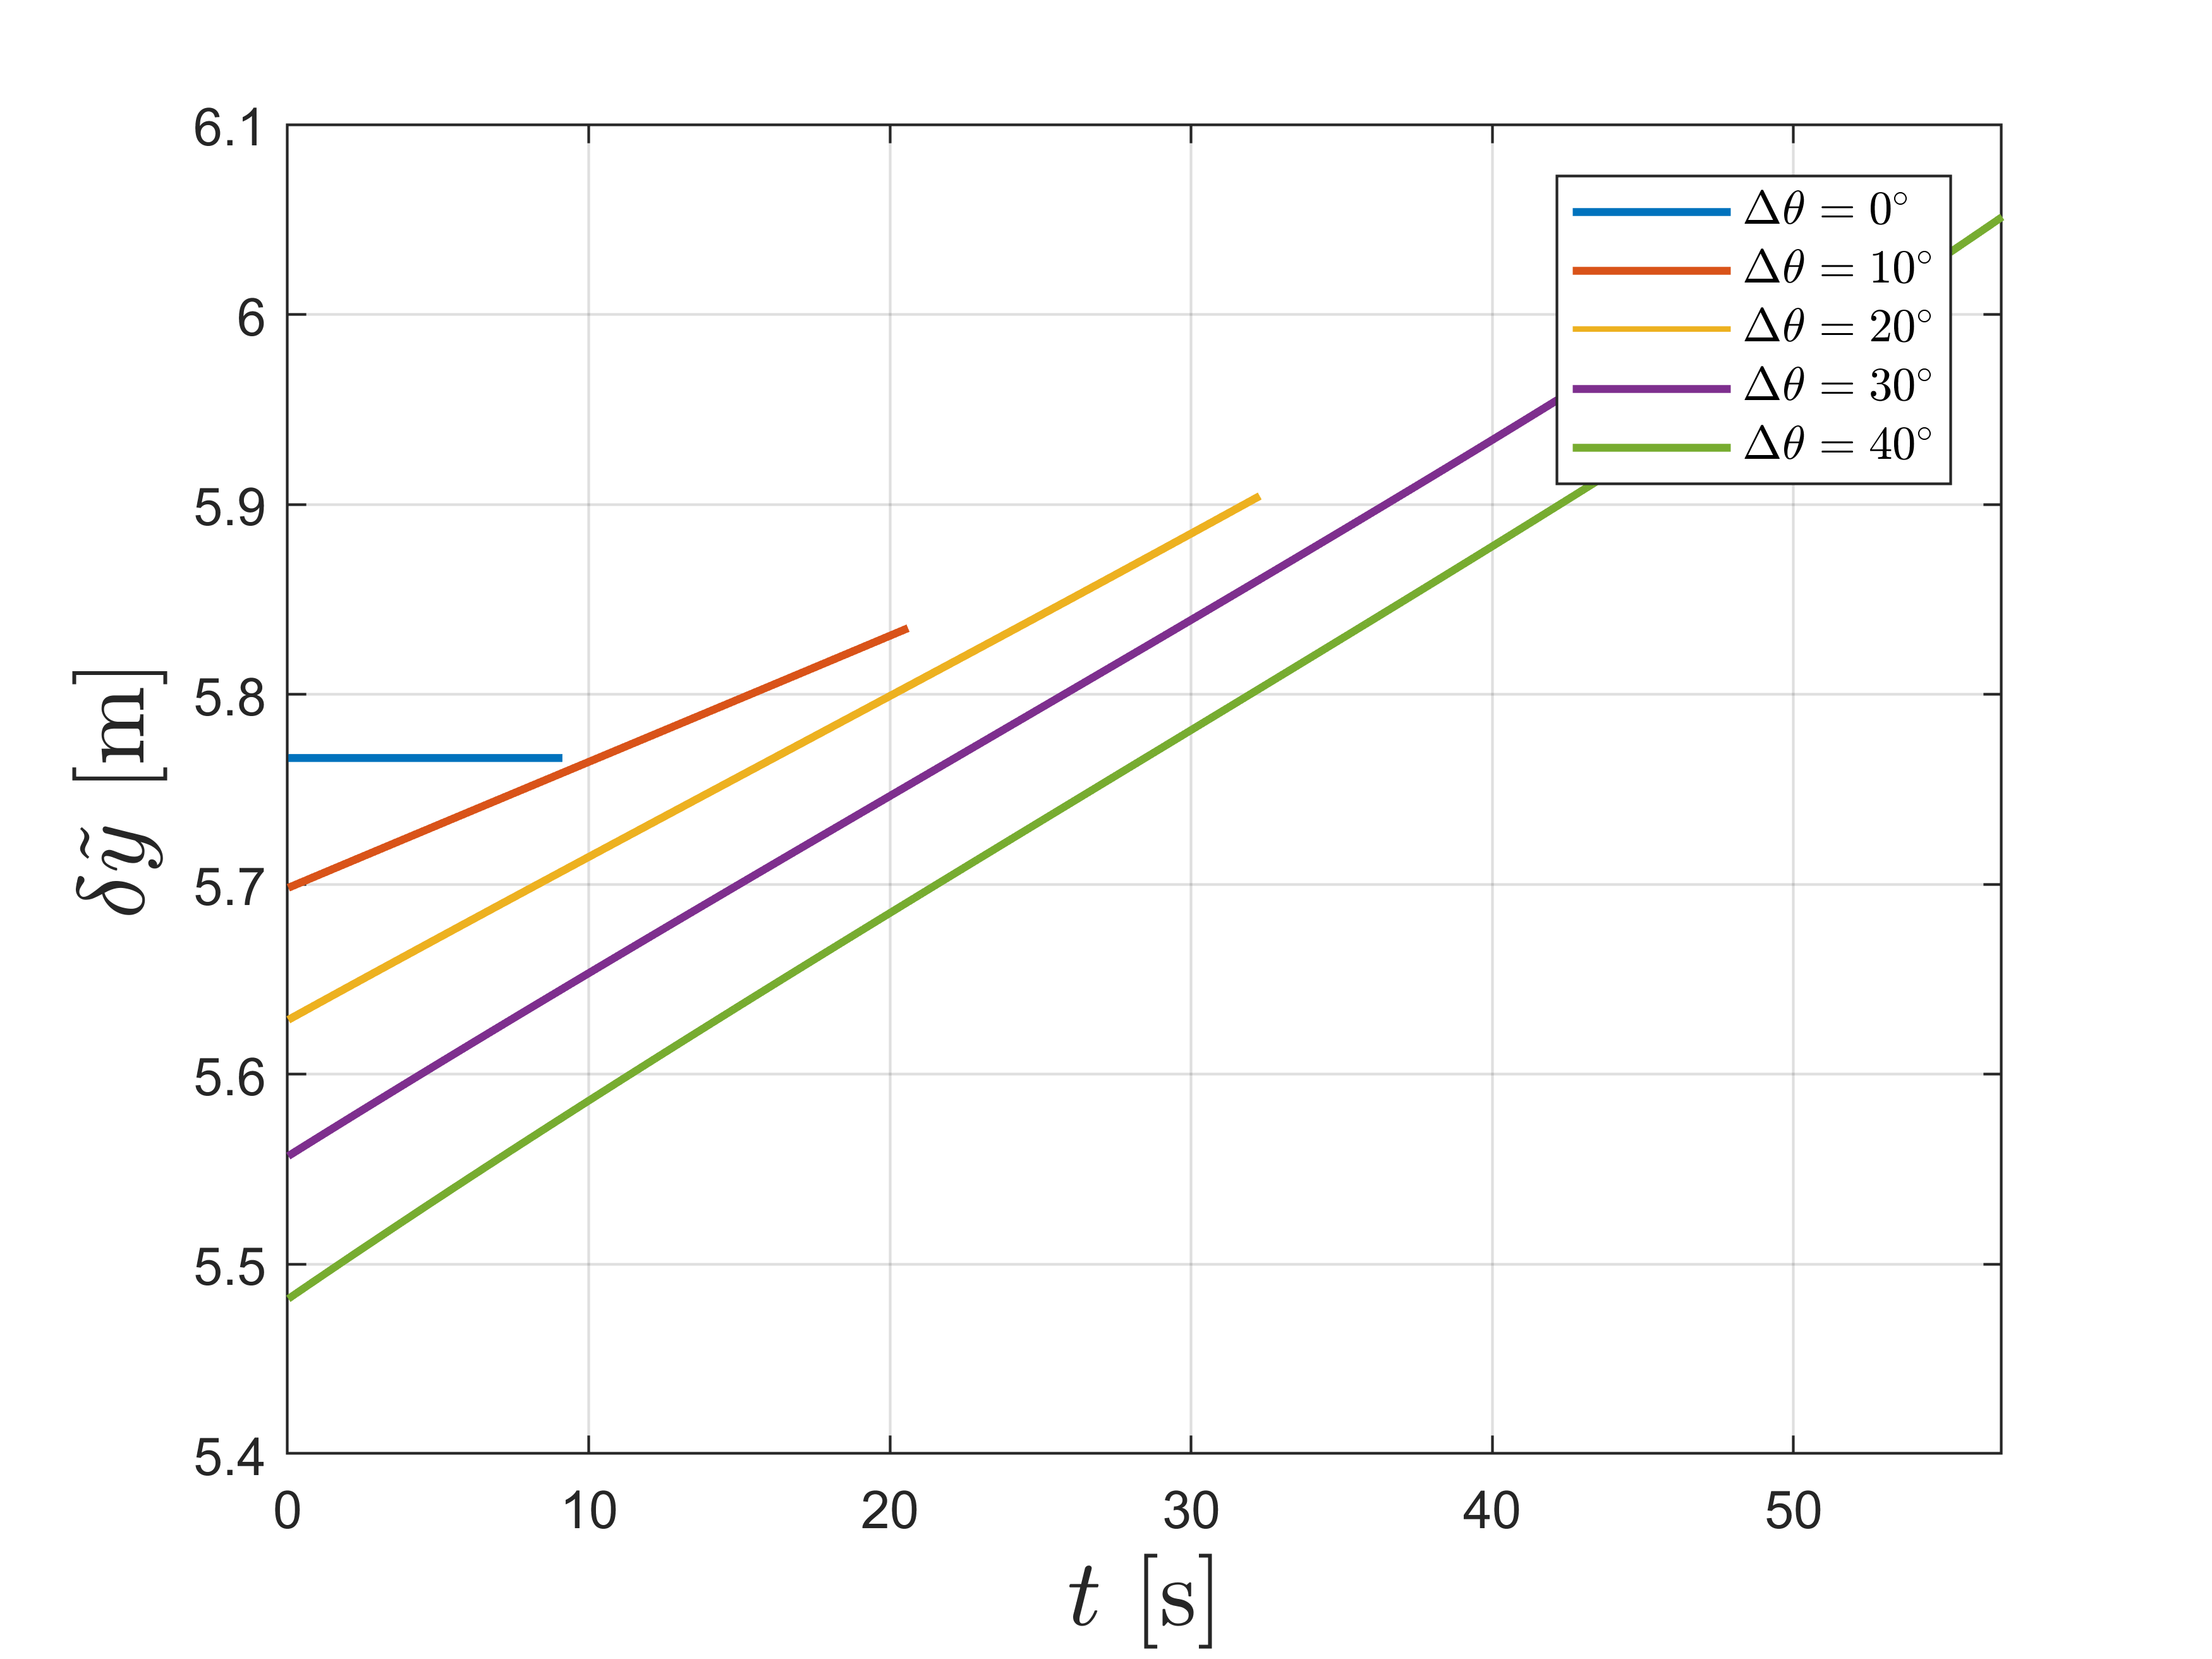
\includegraphics[width=0.45\textwidth]{figs/GSD_y.png}
%   \caption{Cross-track RGS for different starting/ending pitch angles $\theta(t_0)=-\theta(t_f)$ and angular velocities $\omega_{y}$. Target track is $s_g=70 \hspace{3pt} \rm{km}$.}
% 	\label{fig:GSDy}
% \end{figure}
% \begin{figure}[htbp]
%   \centering
%       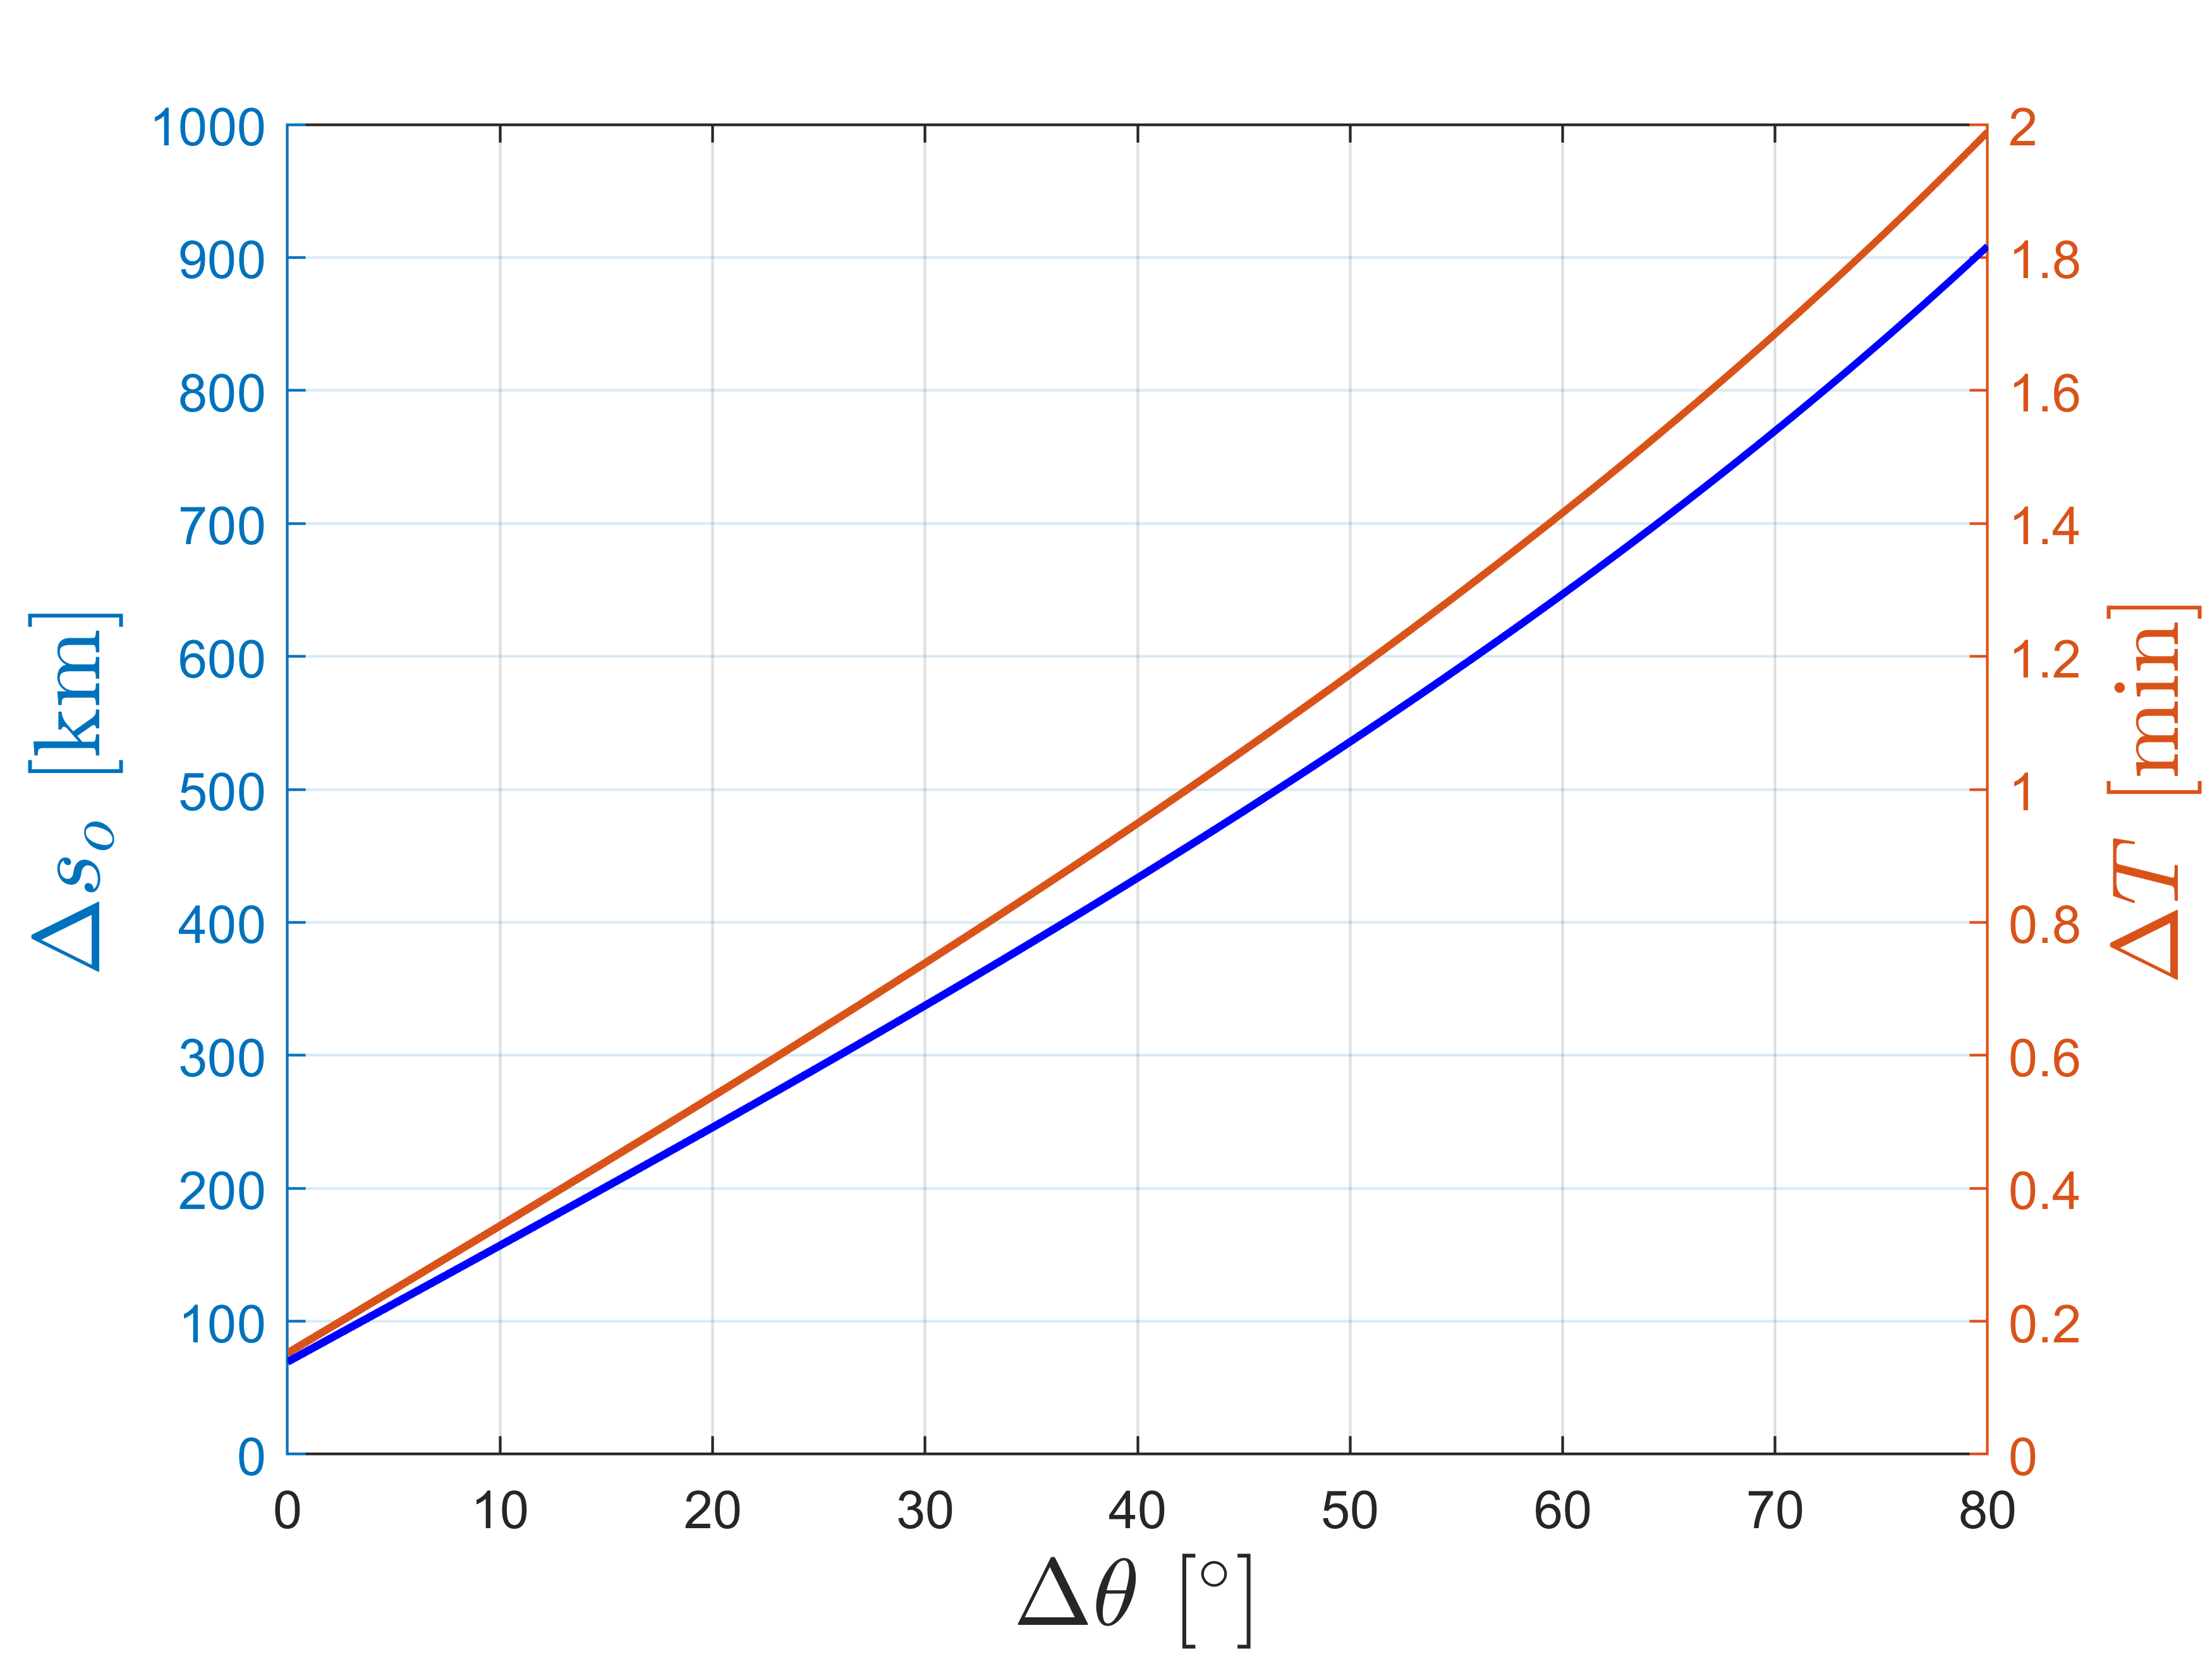
\includegraphics[width=0.45\textwidth]{figs/track_time.png}
%   \caption{In-orbit track distance and observation time vs. starting/ending pitch angles $\theta(T_0)=-\theta(T_f)$ and angular velocities $\omega_{y}$. Target track is $s_g=70 \hspace{3pt} \rm{km}$.}
% 	\label{fig:track_time}
% \end{figure}
% \subsubsection{In-track Slew Maneuver with Perturbations}
% Figures \ref{fig:spatial_time_err} and \ref{fig:GSD_x_err} show how noise in the satellite system causes deviations to the sensor output performance and the nominal reference ground track. Noise is assumed to be Gaussian-distributed with zero mean such that noise due to the spacecraft structure and the actuators (e.g. reaction wheels) is represented with $\delta\boldsymbol{\omega} \sim \mathcal{N}(0, 0.1^{\circ}/\rm{s})$. 
% Table \ref{tab:statistics} shows the statistics for spatial resolution, GSD and pitch angle due to variations in vehicle angular velocity $\boldsymbol{\omega}$. 
% \begin{figure}[htbp]
%   \centering
%       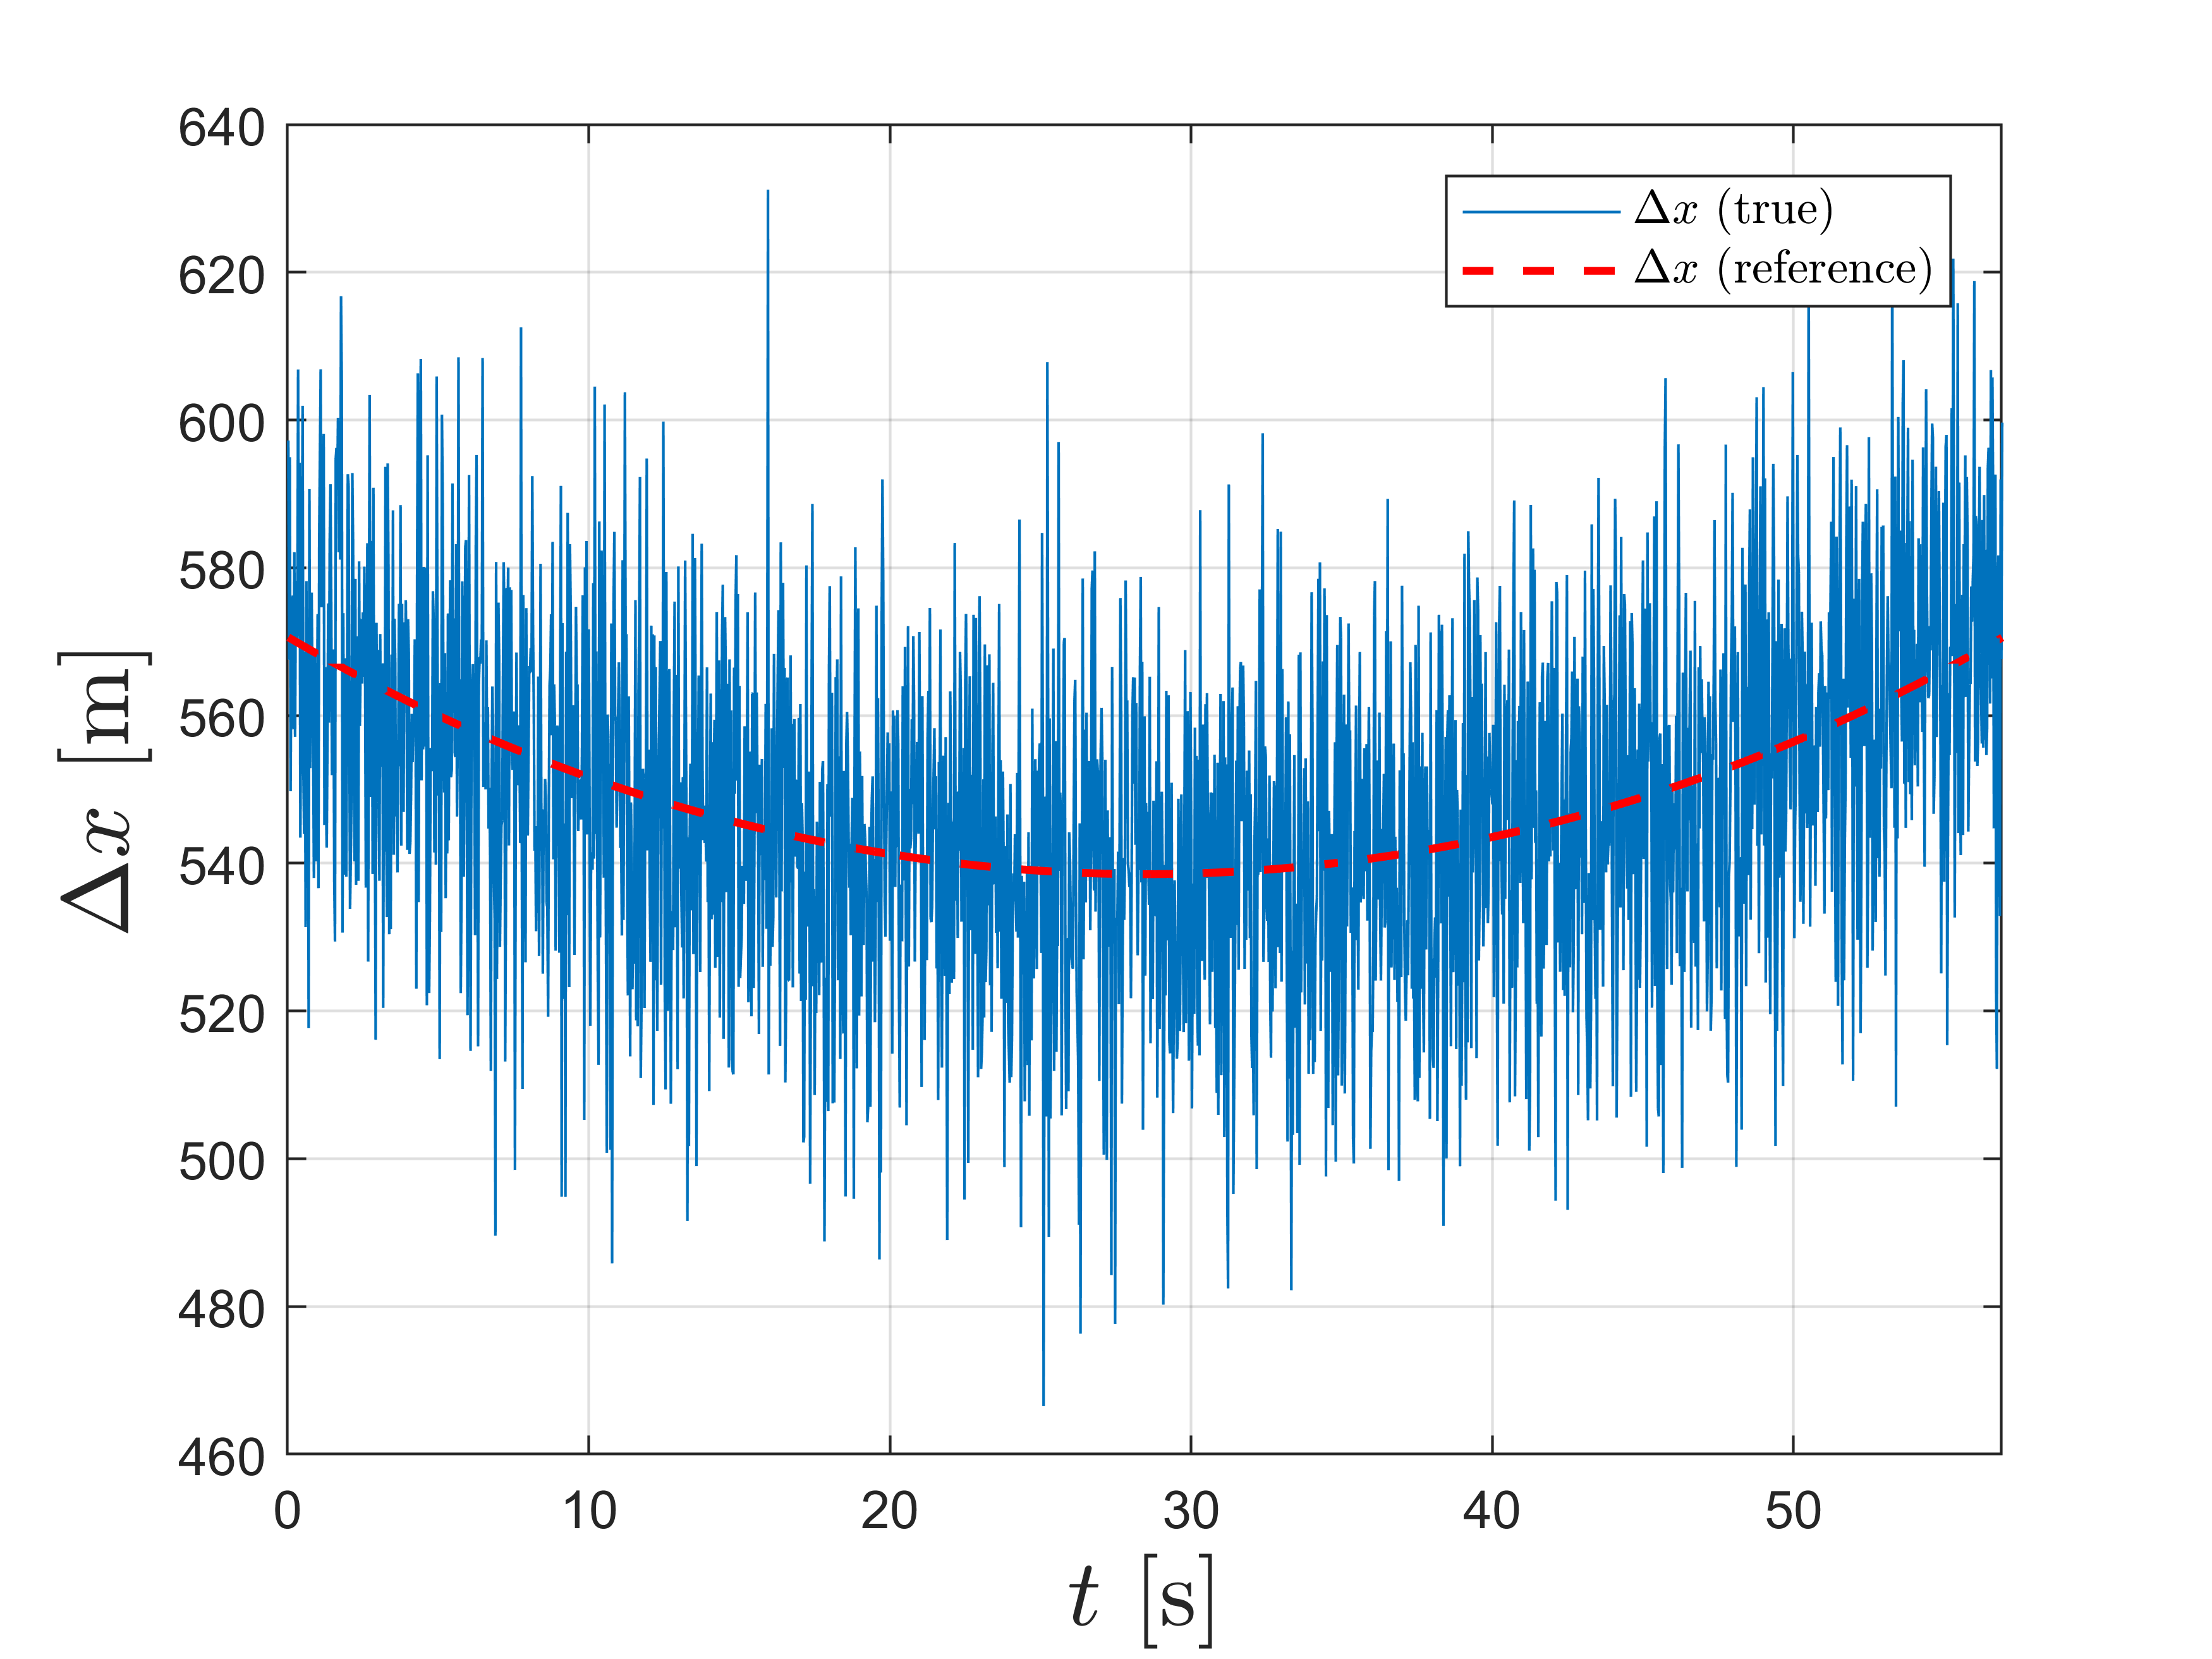
\includegraphics[width=0.45\textwidth]{figs/spatial_time_err.png}
%   \caption{In-track spatial resolution for $\Delta \theta = 40^{\circ}$, $\omega_{y}=-0.7025^{\circ}/\rm{s}$ and $\delta\boldsymbol{\omega} \sim \mathcal{N}(0, 0.1^{\circ}/\rm{s})$.}
% 	\label{fig:spatial_time_err}
% \end{figure}
% \begin{figure}[htbp]
%   \centering
%       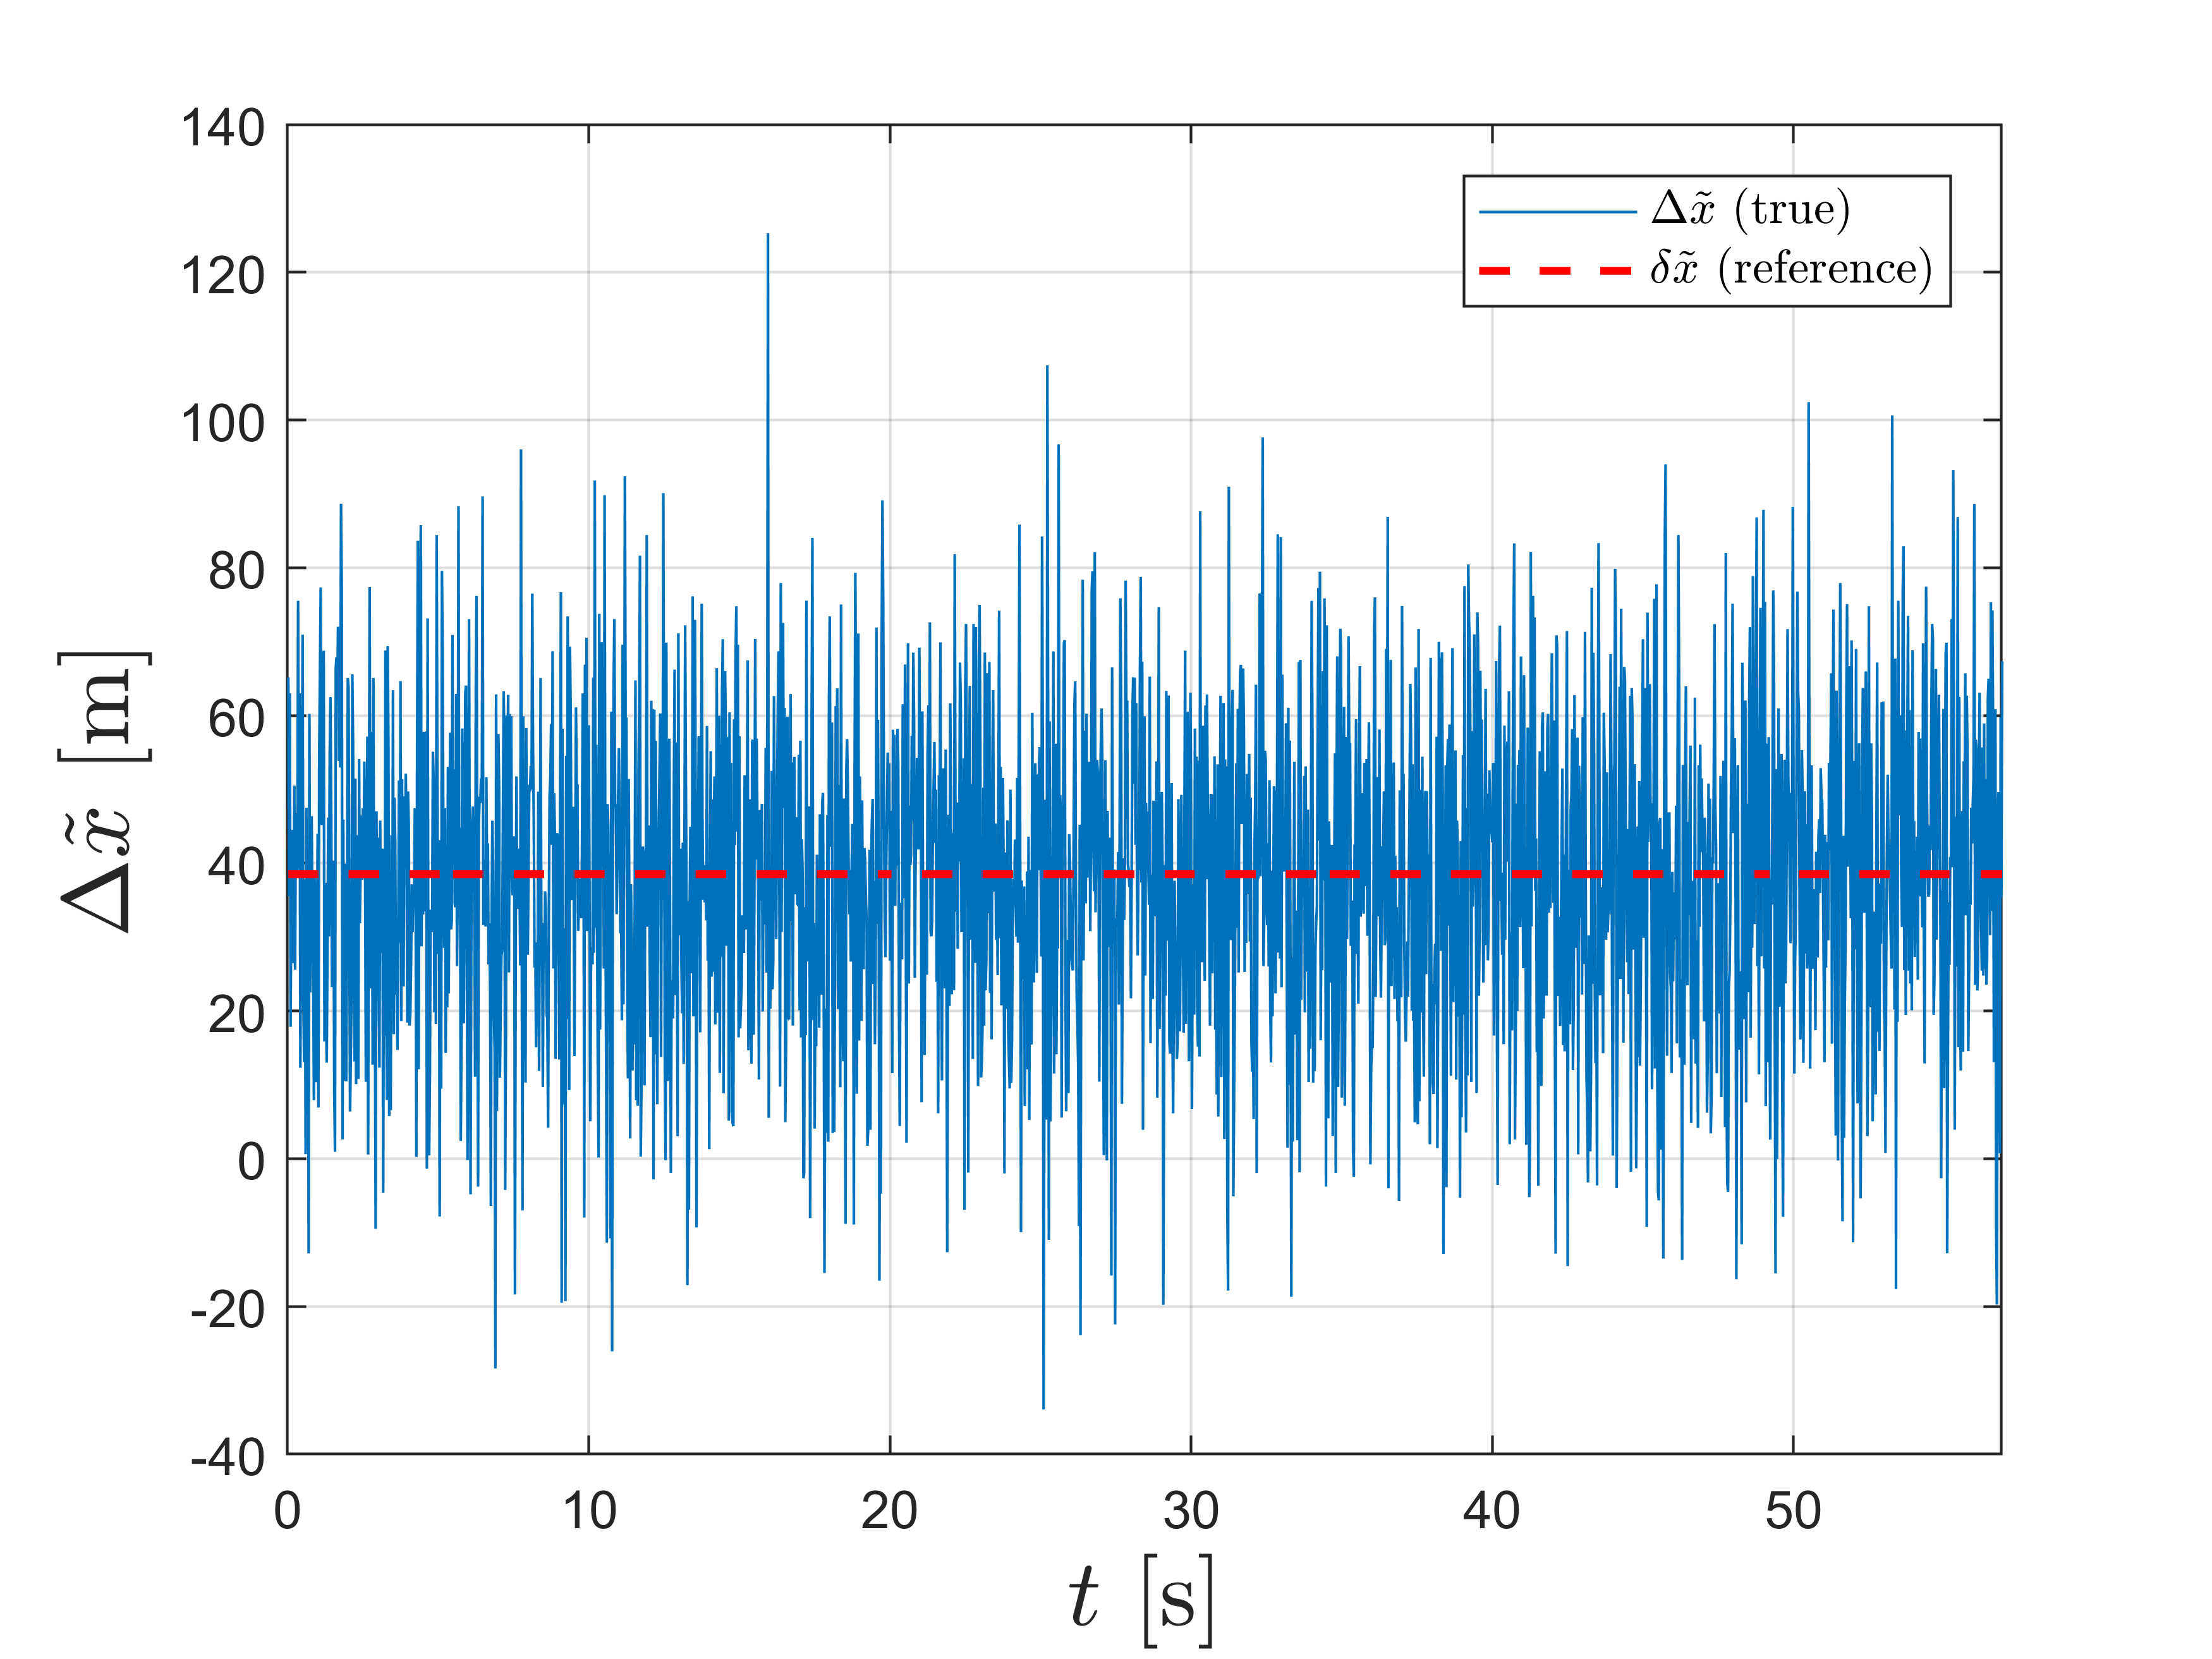
\includegraphics[width=0.45\textwidth]{figs/GSD_x_err.png}
%   \caption{In-track GSD for $\Delta \theta = 40^{\circ}$, $\omega_{y}=-0.7025^{\circ}/\rm{s}$ and $\delta\boldsymbol{\omega} \sim \mathcal{N}(0, 0.1^{\circ}/\rm{s})$.}
% 	\label{fig:GSD_x_err}
% \end{figure}
% \begin{table}[htbp]
% 	\caption{Statistics for satellite spatial imaging performance during slew maneuver}
% 	\label{tab:statistics}
% 	\centering
% 			\begin{tabular}{l r r r r}
% 				\hline
% 				Value & Mean & Standard Deviation & Maximum & Minimum \\
% 				$\Delta x$ & $549.19 \hspace{3pt} \rm{m}$ & $23.84 \hspace{3pt} \rm{m}$ & $632.46 \hspace{3pt} \rm{m}$ & $442.43 \hspace{3pt} \rm{m}$ \\
% 				$\Delta y$ & $64.28 \hspace{3pt} \rm{m}$ & $21.62 \hspace{3pt} \rm{m}$ & $141.00 \hspace{3pt} \rm{m}$ & $-9.84 \hspace{3pt} \rm{m}$ \\
% 				$P_{y}$ & $71.64 \hspace{3pt} \rm{km}$ & $1.33 \hspace{3pt} \rm{km}$ & $74.71 \hspace{3pt} \rm{km}$ & $70.17 \hspace{3pt} \rm{km}$ \\
% 				$\delta x$ & $510.48 \hspace{3pt} \rm{m}$ & $9.51 \hspace{3pt} \rm{m}$ & $532.37 \hspace{3pt} \rm{m}$ & $500.00 \hspace{3pt} \rm{m}$ \\
% 				$\tilde{x}$ & $38.71 \hspace{3pt} \rm{m}$ & $21.86 \hspace{3pt} \rm{m}$ & $102.60 \hspace{3pt} \rm{m}$ & $-58.25 \hspace{3pt} \rm{m}$ \\
% 				$\tilde{y}$ & $5.36 \hspace{3pt} \rm{m}$ & $21.61 \hspace{3pt} \rm{m}$ & $82.36 \hspace{3pt} \rm{m}$ & $-69.04 \hspace{3pt} \rm{m}$ \\
% 				\hline
% 				\end{tabular}
% \end{table}
\subsubsection{Target SNR}
\begin{figure}[htbp]
  \centering
      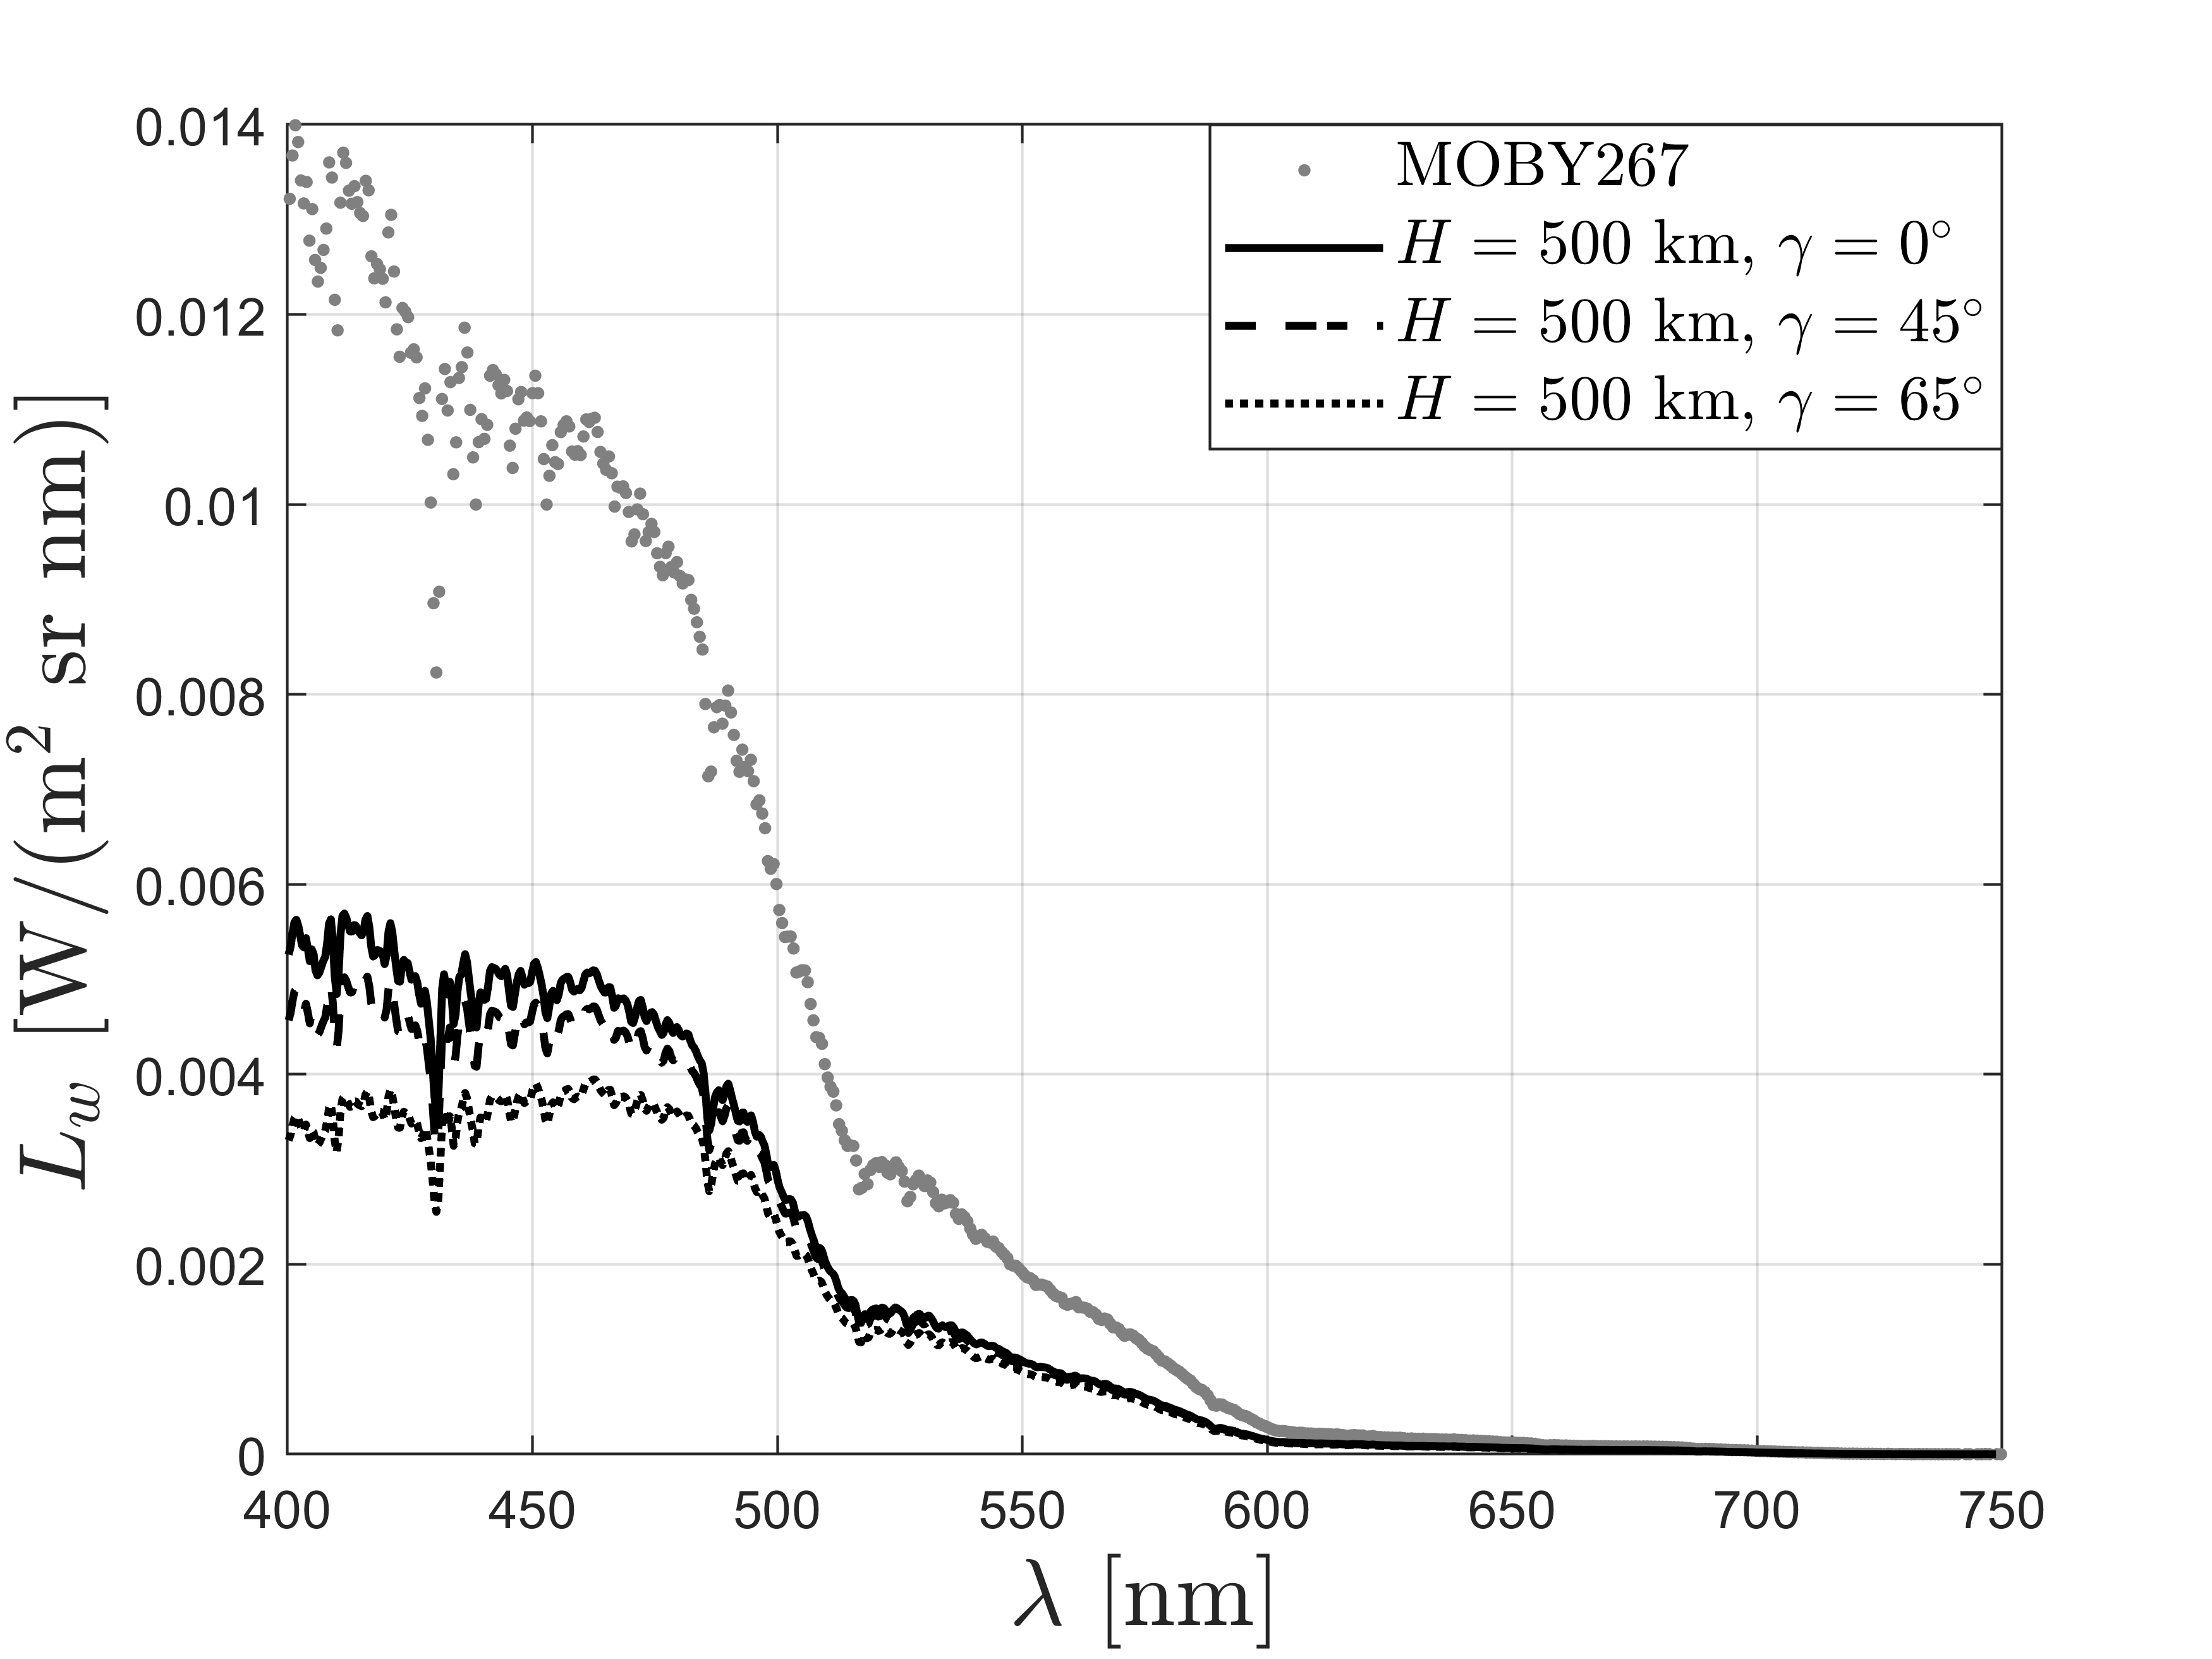
\includegraphics[width=0.45\textwidth]{figs/radiance.png}
  \caption{Water-leaving radiance $L_w$ measured by MOBY267 and estimated at ToA for different viewing angles $\gamma$.}
	\label{fig:signal}
\end{figure}
To simulate typical water conditions to be observed by HYPSO-1's hyperspectral imager and its corresponding estimate of SNR, we have used water-leaving radiance measurements from the Marine Optical BuoY (MOBY) with deployment number $267$ off the coast of Hawaii. The data sets are publicly available, mainly used for vicarious calibration of EO remote sensing data \cite{Clark2002}. The chosen measurements are time-stamped at 21:11:38 GMT on 3 July 2019 and a spline curve is fitted to the calibrated data in the wavelength range of $348.8391-749.7629 \hspace{3pt} \rm{nm}$ to match the resolution of the hyperspectral imager. Figure \ref{fig:signal} shows the point measurements and simulated water-leaving radiance for viewing angles $\gamma$ as seen at Top-of-Atmosphere (ToA), assuming that the water-leaving radiance diminishes due to the water refraction index and the atmospheric transmittance consisting of only the Rayleigh optical thickness \cite{Bucholtz1995}. 
% It is also assumed that photon flux is constant during the short exposure time $\tau$. 
% 12 binning, 160 binned pixels, 1936/12 = 160 pixels, 500/160=3.1 nm per binned pixel.
% \begin{figure}[htbp]
%   \centering
%       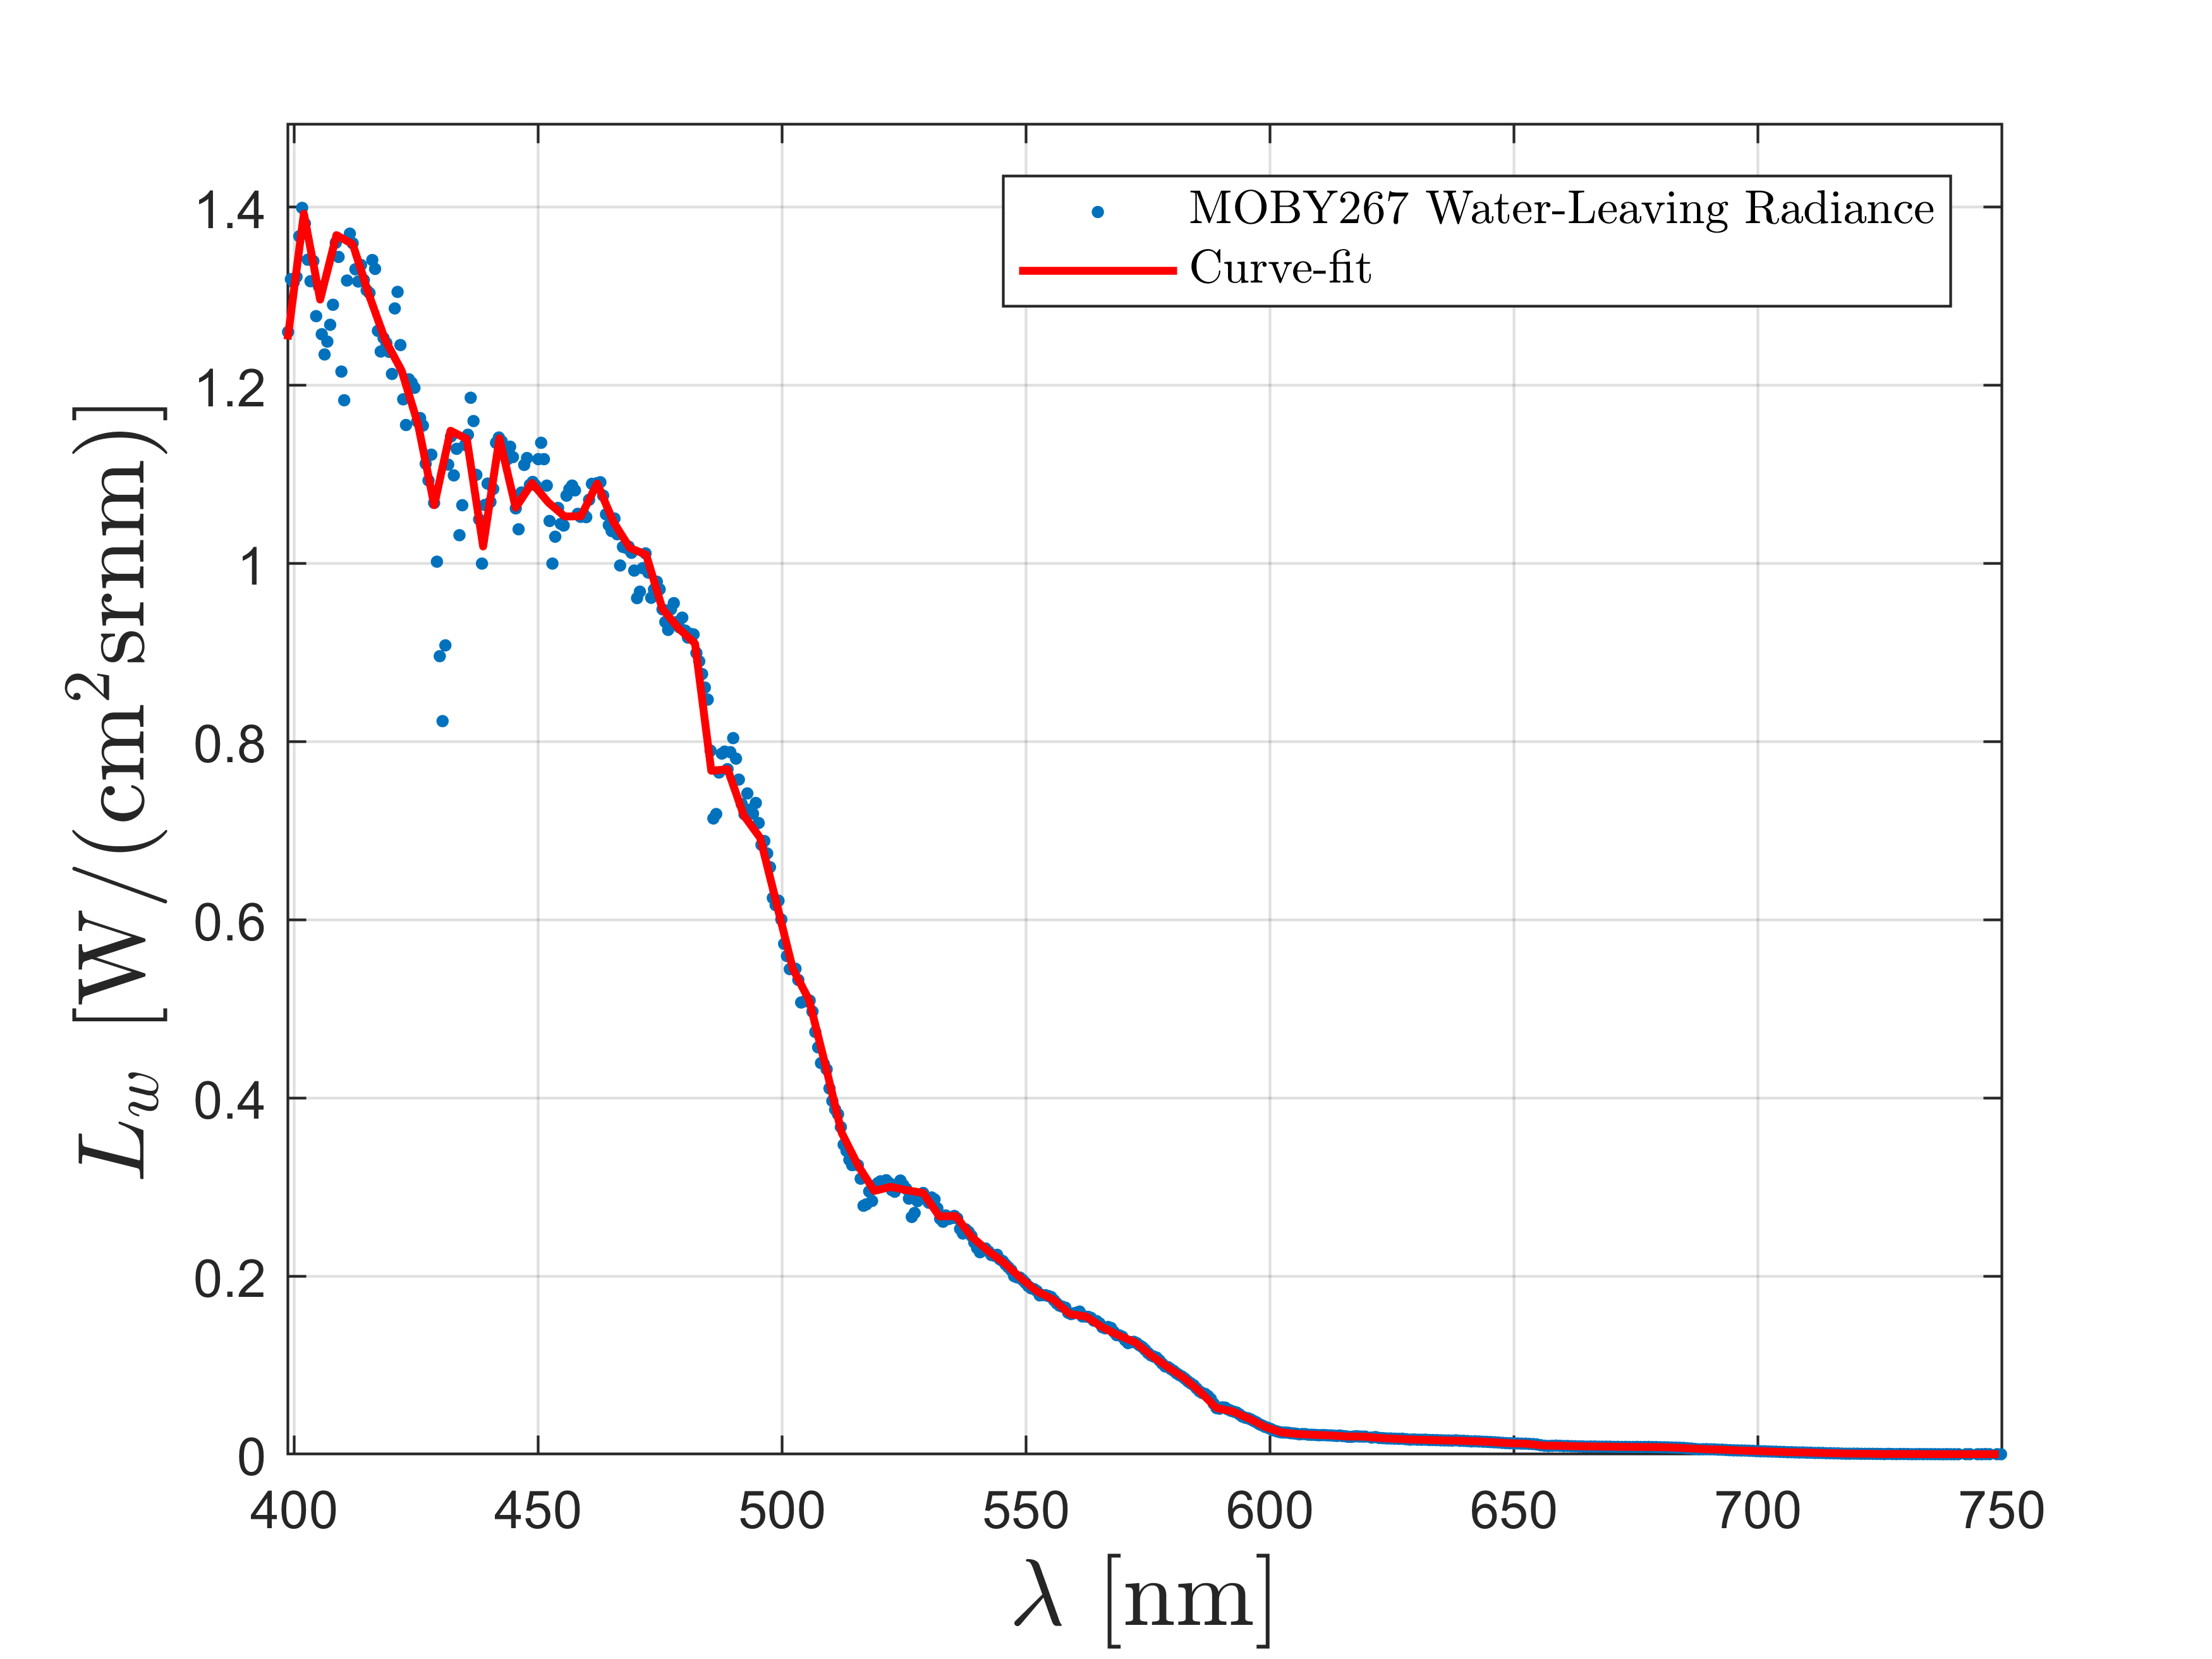
\includegraphics[width=0.45\textwidth]{figs/MOBY.png}
%   \caption{Water-leaving radiance data collected by MOBY. Red line shows a curve fit to the data at spectral resolution .}
% 	\label{fig:moby}
% \end{figure}
\begin{figure}[htbp]
  \centering
      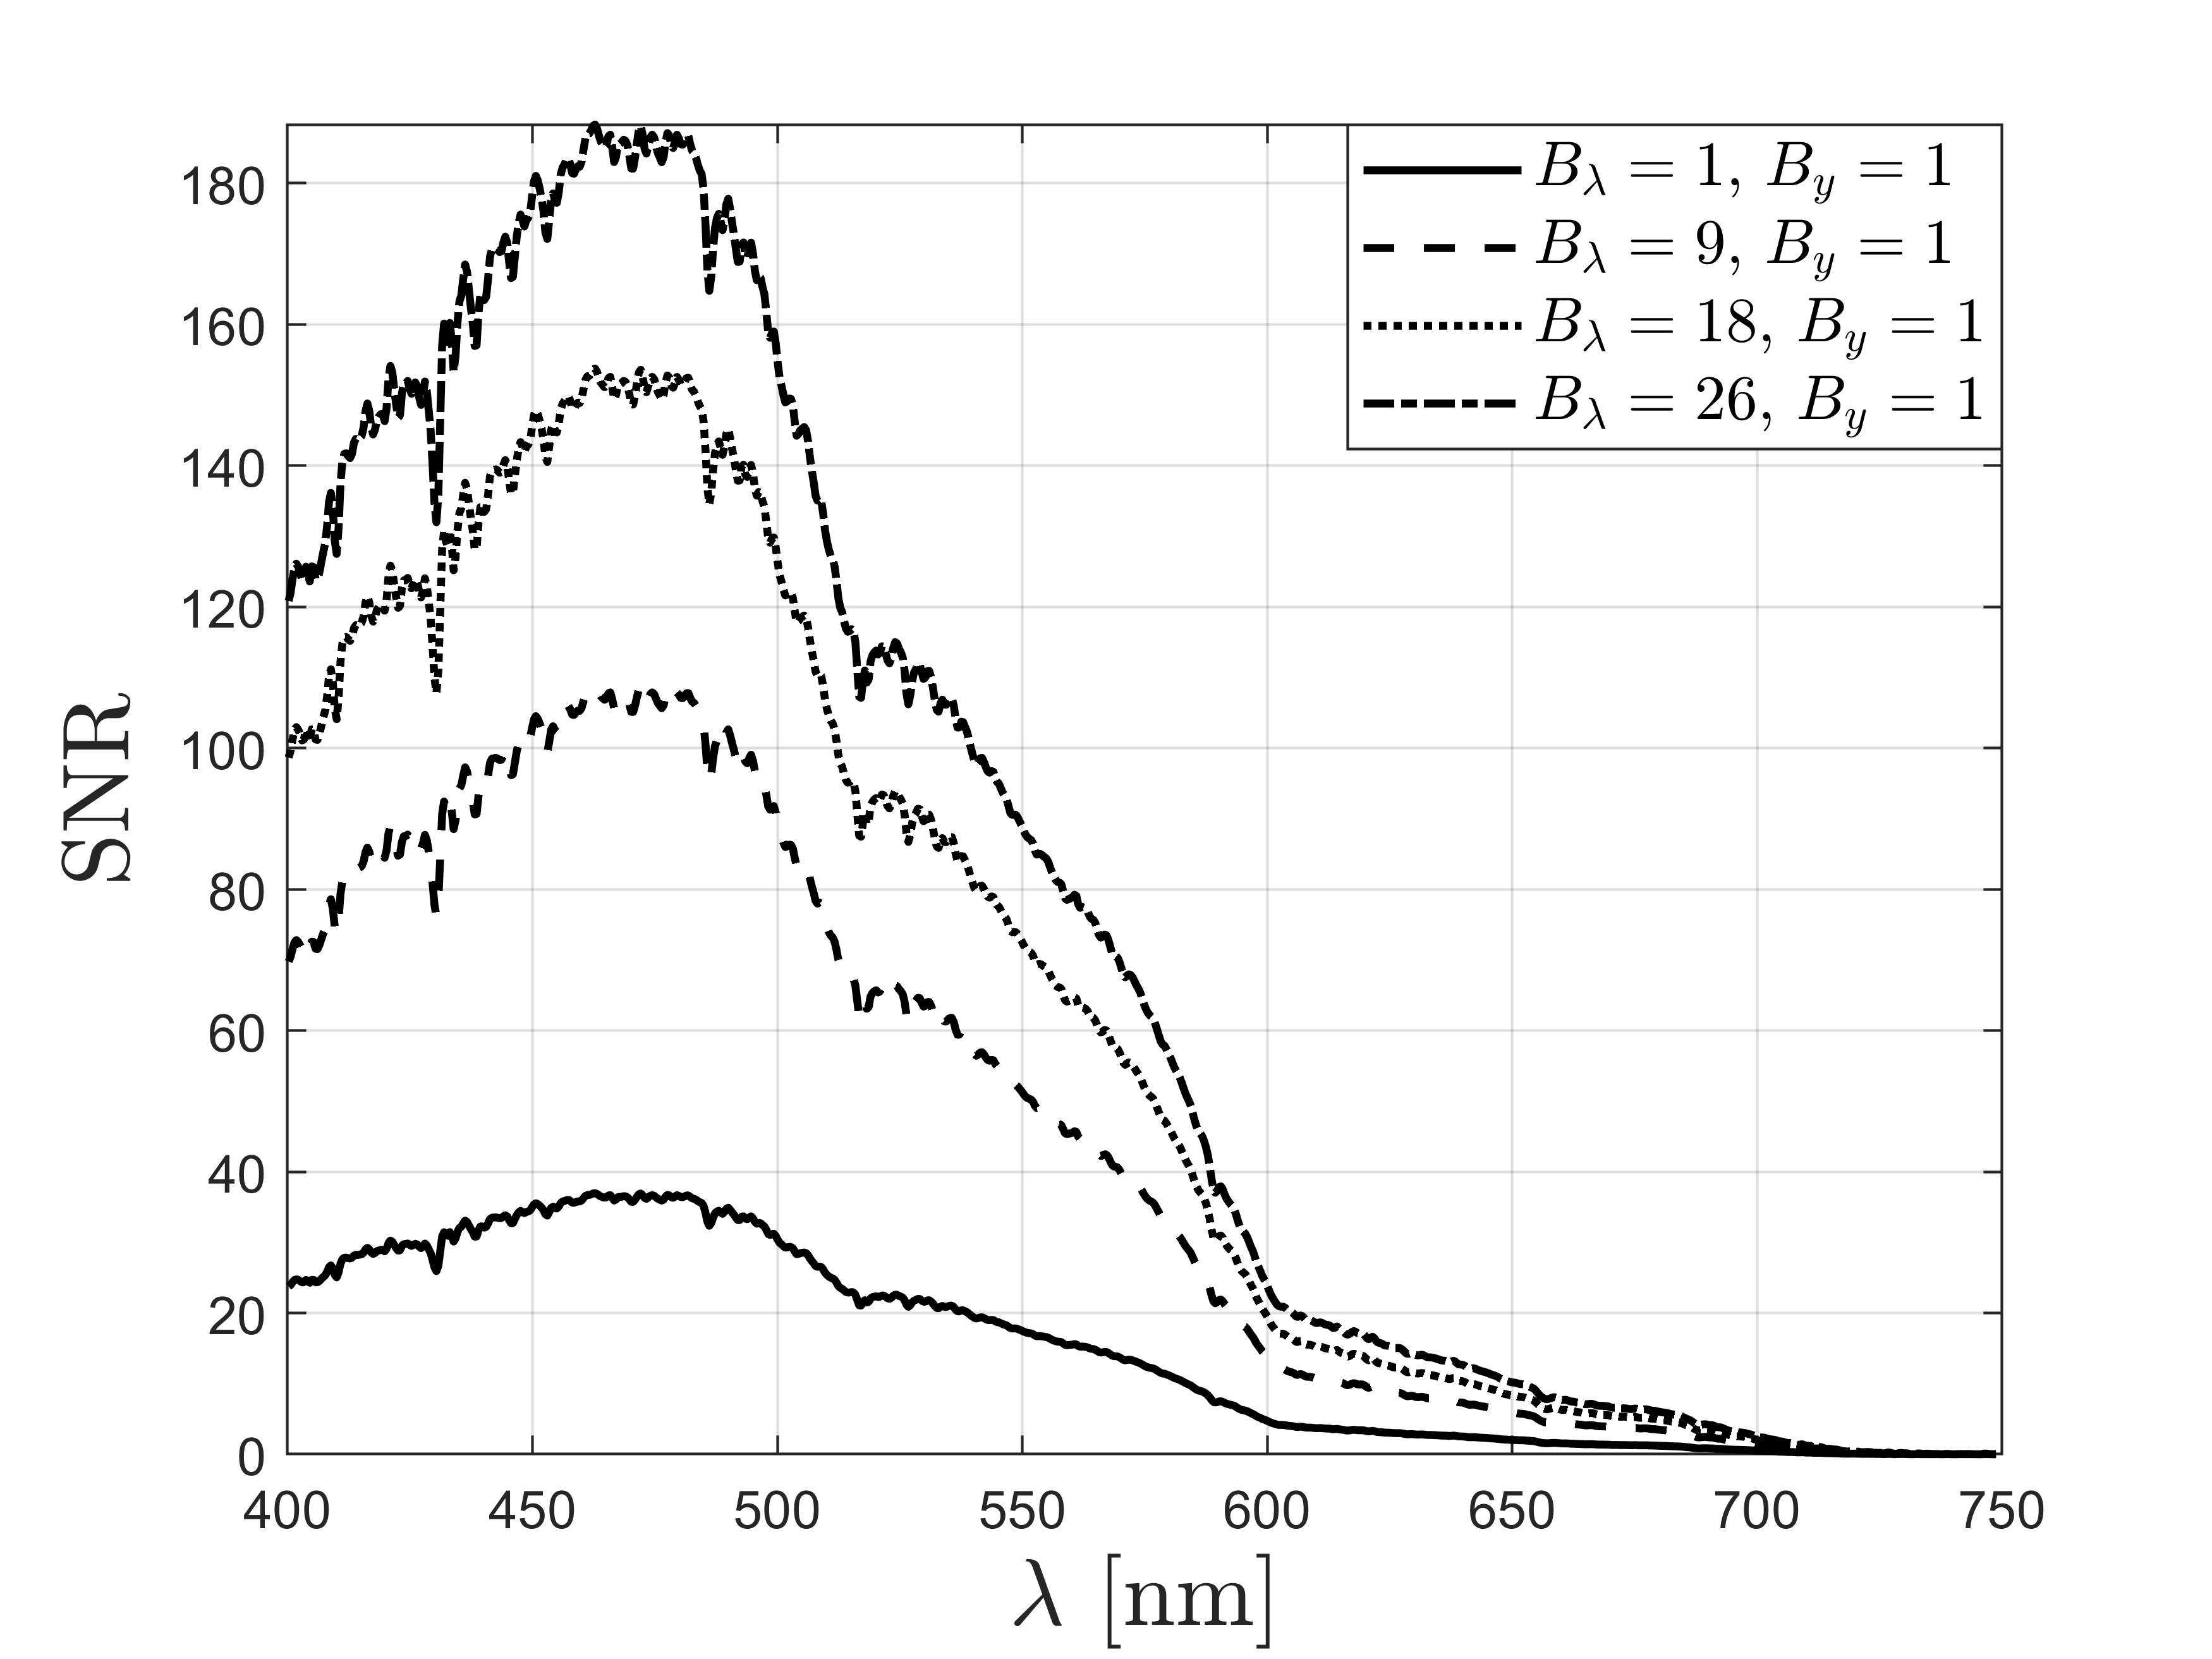
\includegraphics[width=0.45\textwidth]{figs/snr.png}
  \caption{SNR of $L_w$ as seen at ToA with selected number of binning operations per pixel.}
	\label{fig:fred_snr2}
\end{figure}

Using Eqs. (\ref{eq:photons}), (\ref{eq:photons2}) and (\ref{eq:snr}), Figure \ref{fig:fred_snr2} shows the estimated SNR in the $400-750\hspace{3pt} \rm{nm}$ spectral range for the hyperspectral imager sensing the radiance $L=L_w$ at ToA with $\gamma=0^{\circ}$ and $\tau=41.4 \hspace{3pt} \rm{ms}$. It is shown how binning  pixels in the spectral direction increases the SNR. With no binning and at $B_\lambda=9$ we have $BP=3.33 \hspace{3pt} \rm{nm}$ while $B_\lambda=18$ and $B_\lambda=26$ result in $BP=6.67 \hspace{3pt} \rm{nm}$ and $BP=10 \hspace{3pt} \rm{nm}$, respectively. 
% Blue curve shows SNR per unbinned pixel. Red curve shows SNR for $B_\lambda=N_w$ binned pixels along the spectral direction. Green curve shows SNR for binned pixels with $B_\lambda=3 \times N_w$ along the spectral direction to achieve $BP=10 \hspace{3pt} \rm{nm}$. Without binning in cross-track spatial dimension $B_y$, the optical spatial resolution of a pixel for this case is $\delta x \times \delta y = 500 \hspace{3pt} \rm{m} \times 57.65 \hspace{3pt} \rm{m}$. Magenta curve shows a square window of pixels $9\times 9$ with bandpass of $BP=3.33 \hspace{3pt} \rm{nm}$, that means $B_y=9$ pixels are binned in the spatial direction. Optical spatial resolution for this cases is $\delta x \times B_y\delta y = 500 \hspace{3pt} \rm{m} \times 518.65 \hspace{3pt} \rm{m}$.
It is worth mentioning that the simulated SNR does not take into account the total radiance at ToA which includes light due to predominantly aerosol scattering and sun reflection \cite{Franz2007}. Atmospheric scattering of the solar radiation into the hyperspectral imager's path will typically be 10 to 20 times larger at $500 \hspace{3pt} \rm{km}$ altitude \cite{Corson2008, Gao2012}. With this assumption, $20\cdot L_w$ or $\sqrt{20}$ times the highest SNR of $36.97$ at $463 \hspace{3pt} \rm{nm}$ would be approximately $\sqrt{20}\cdot36.97=165.33$ which is still below the saturation at SNR of $181.6$ for an unbinned pixel. Further, the effective SNR is expected to increase due to more overlapping frames during a slew maneuver. For an ideal slew maneuver with $\omega_y=0.754^{\circ}\rm{/s}$, rendering $12$ overlapping frames, results in up to $\sqrt{12}$ times higher SNR for an image pixel containing the same scene.
% For instance, when observing the radiance $L_w$ presented in Figure \ref{fig:signal} which gives the photon flux of $20703 \hspace{3pt} \rm{e^{-}/s}$ into each pixel assuming ToA radiance is 10 times larger, then the exposure time setting may be constrained to be $\tau<1.59 \hspace{3pt} \rm{s}$.

% For example, by binning $B_\lambda=3 N_\lambda = 26$ and keeping $B_y=1$ then the bandpass becomes $BP=10 \hspace{3pt} \rm{nm}$ and SNR at $495.5 \hspace{3pt} \rm{nm}$ increases with $73 \%$ compared to the case with $B_\lambda=N_\lambda=8.67$ and $BP=3.34 \hspace{3pt} \rm{nm}$. 
% Figure \ref{fig:fred_snr3} shows the calculated SNR of water-leaving target radiance for a square window of pixels $N_\lambda \times N_y = 26 \times 26$ and $BP=10 \hspace{3pt} \rm{nm}$. Optical spatial resolution for this case is $\delta x \times B_y \delta y = 500 \hspace{3pt} \rm{m} \times 1498.1 \hspace{3pt} \rm{m}$.
% \begin{figure}[htbp]
%   \centering
%       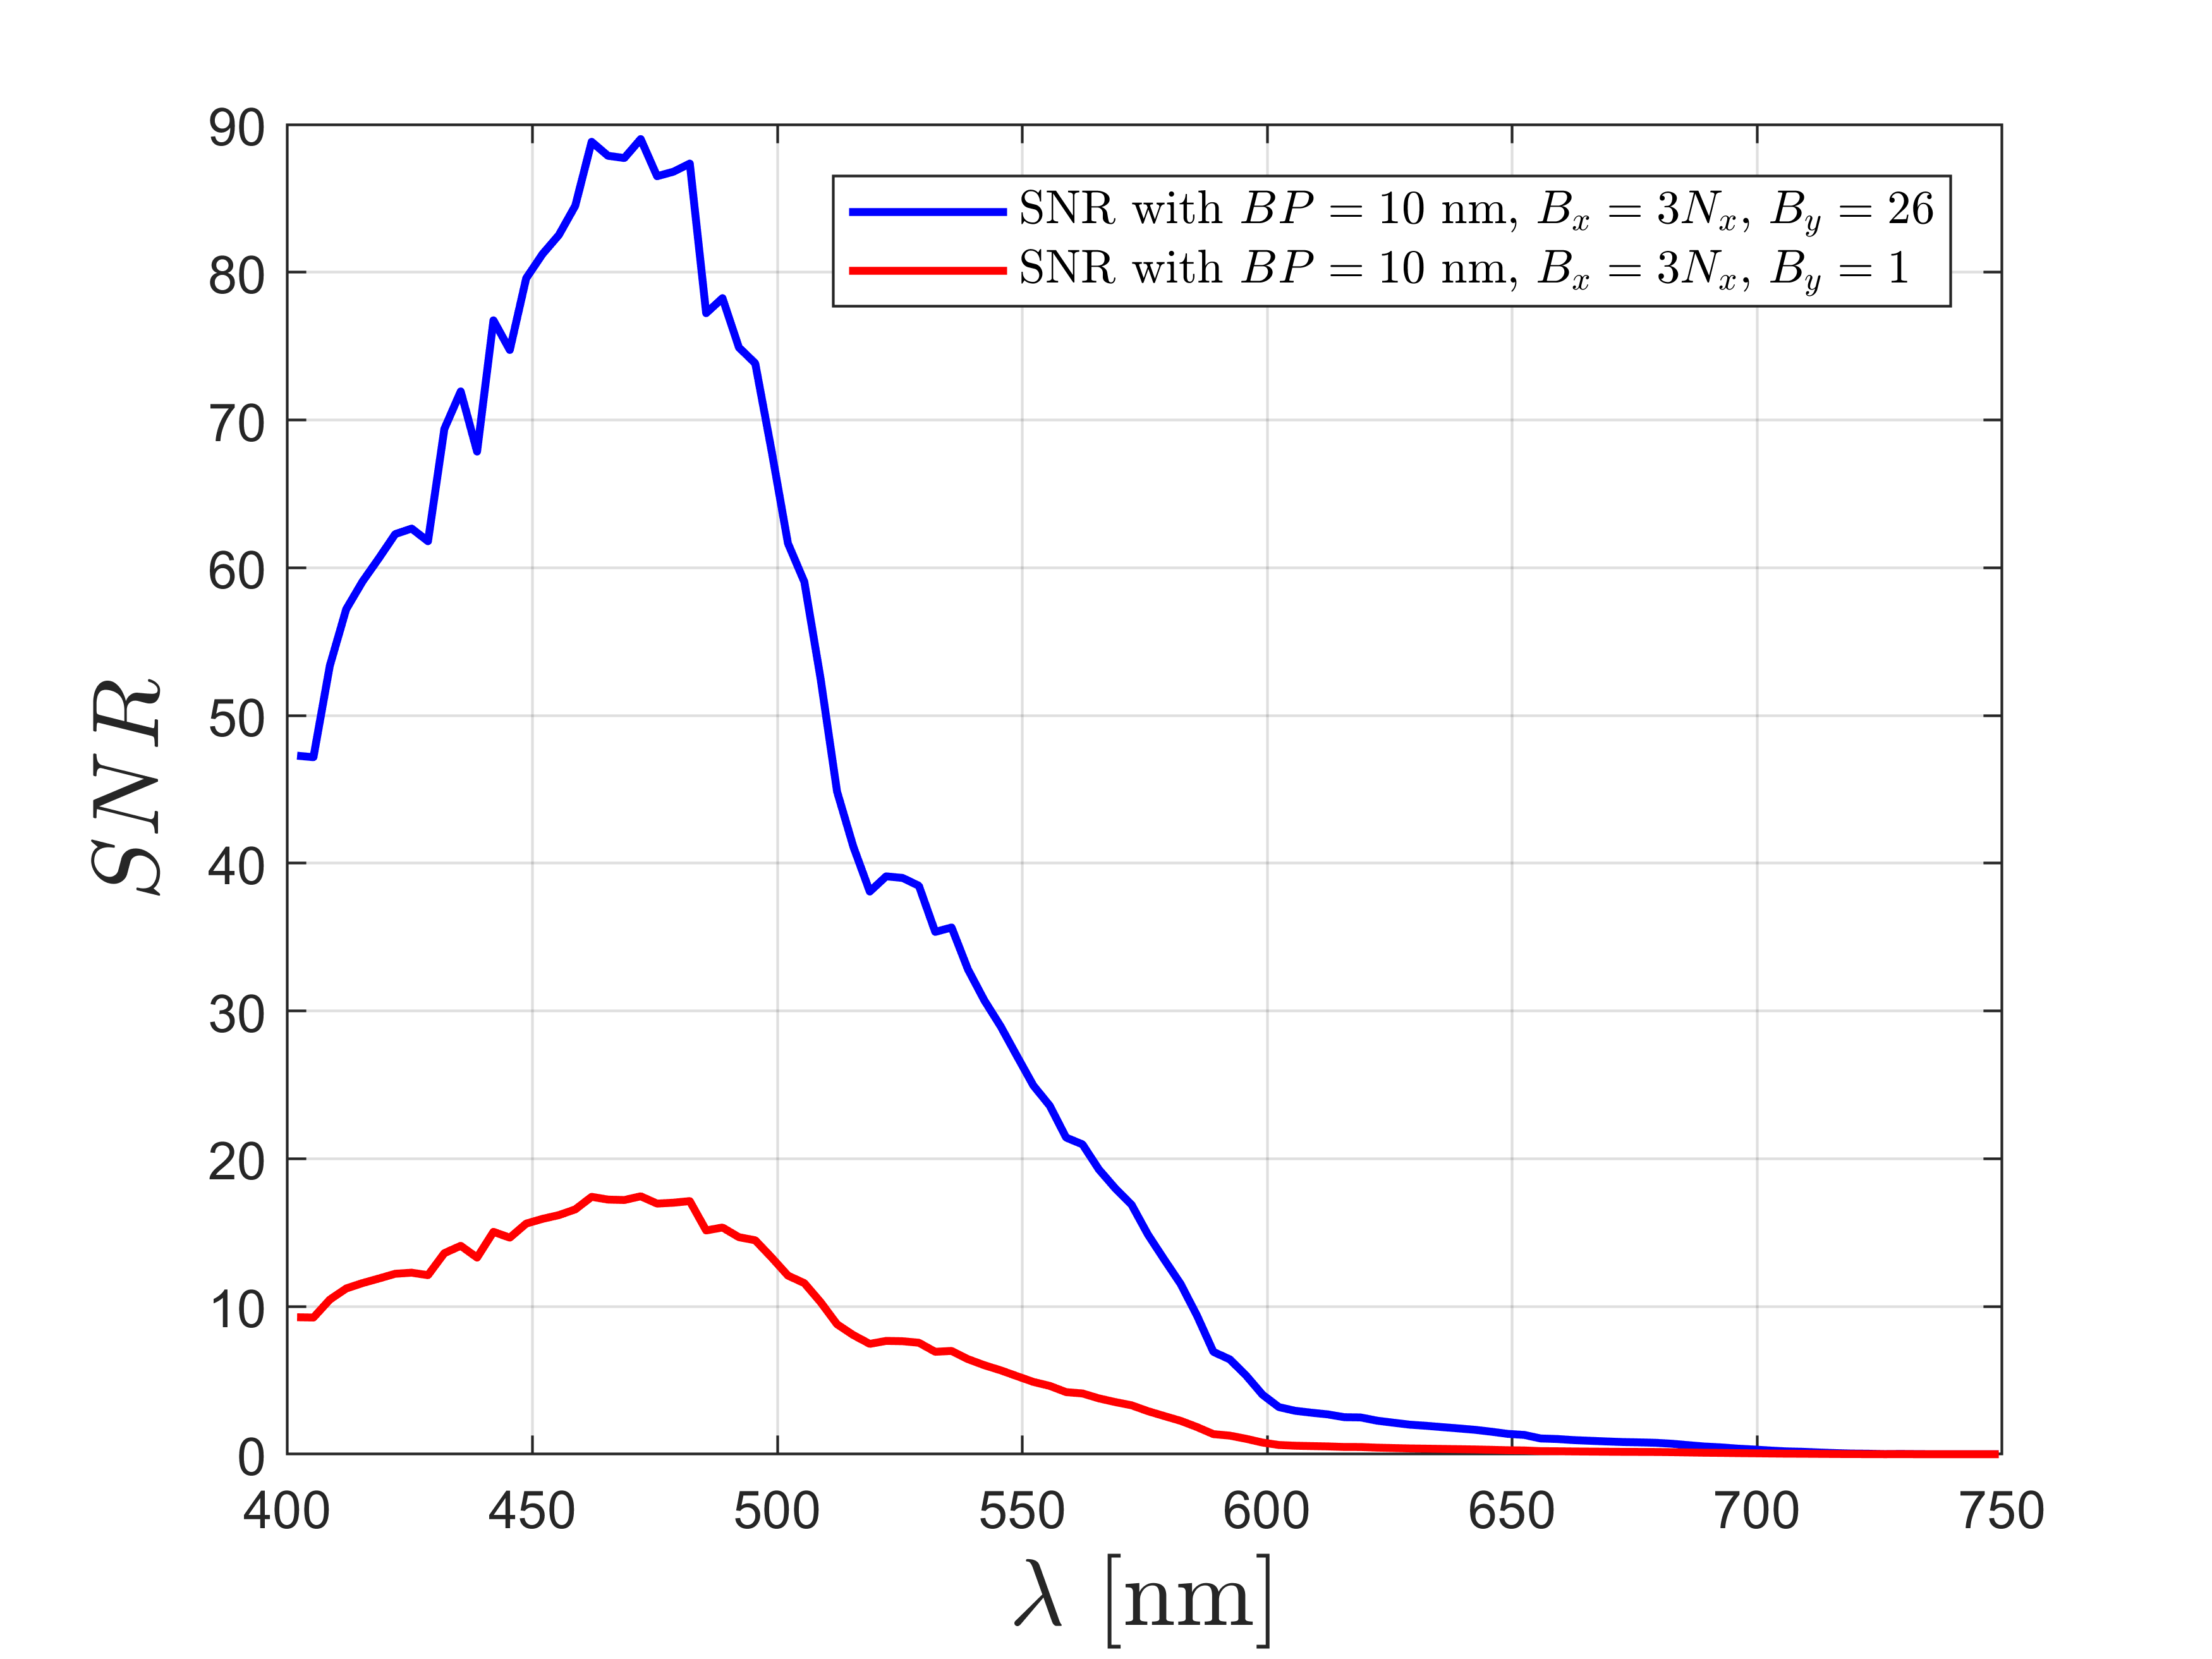
\includegraphics[width=0.45\textwidth]{figs/SNR_Fred2.png}
%   \caption{SNR for binned square window of pixels is shown in blue where $N_\lambda \times N_y = 26 \times 26$ and $BP=10 \hspace{3pt} \rm{nm}$. Red curve shows SNR for a window of pixels with $N_\lambda \times N_y = 26 \times 1$ and $BP=10 \hspace{3pt} \rm{nm}$.}
% 	\label{fig:fred_snr3}
% \end{figure}


% As shown in Fig. \ref{fig:snr_lambda}, if there are $13$ overlapping pixels, then SNR at $495.5 \hspace{3pt} \rm{nm}$ is 30.16 and increases with $261 \%$ compared to the case with unbinned pixels. Furthermore if there are four satellites with $13$ overlapping pixels at same altitude $500\hspace{3pt} \rm{km}$ then the SNR is 176.77 which is an increase of $621 \%$ compared to the case with non-overlapped pixels. SNR is then 1.017 at $619 \hspace{3pt} \rm{nm}$ while for non-overlapped case with unbinned pixels the SNR is only $0.2822$ at the same wavelength. If there are additional four pixels that overlap from four other satellites with same viewing angles, then SNR is $>1$ at $652.4 \hspace{3pt} \rm{nm}$.
% \begin{figure}[htbp]
%   \centering
%       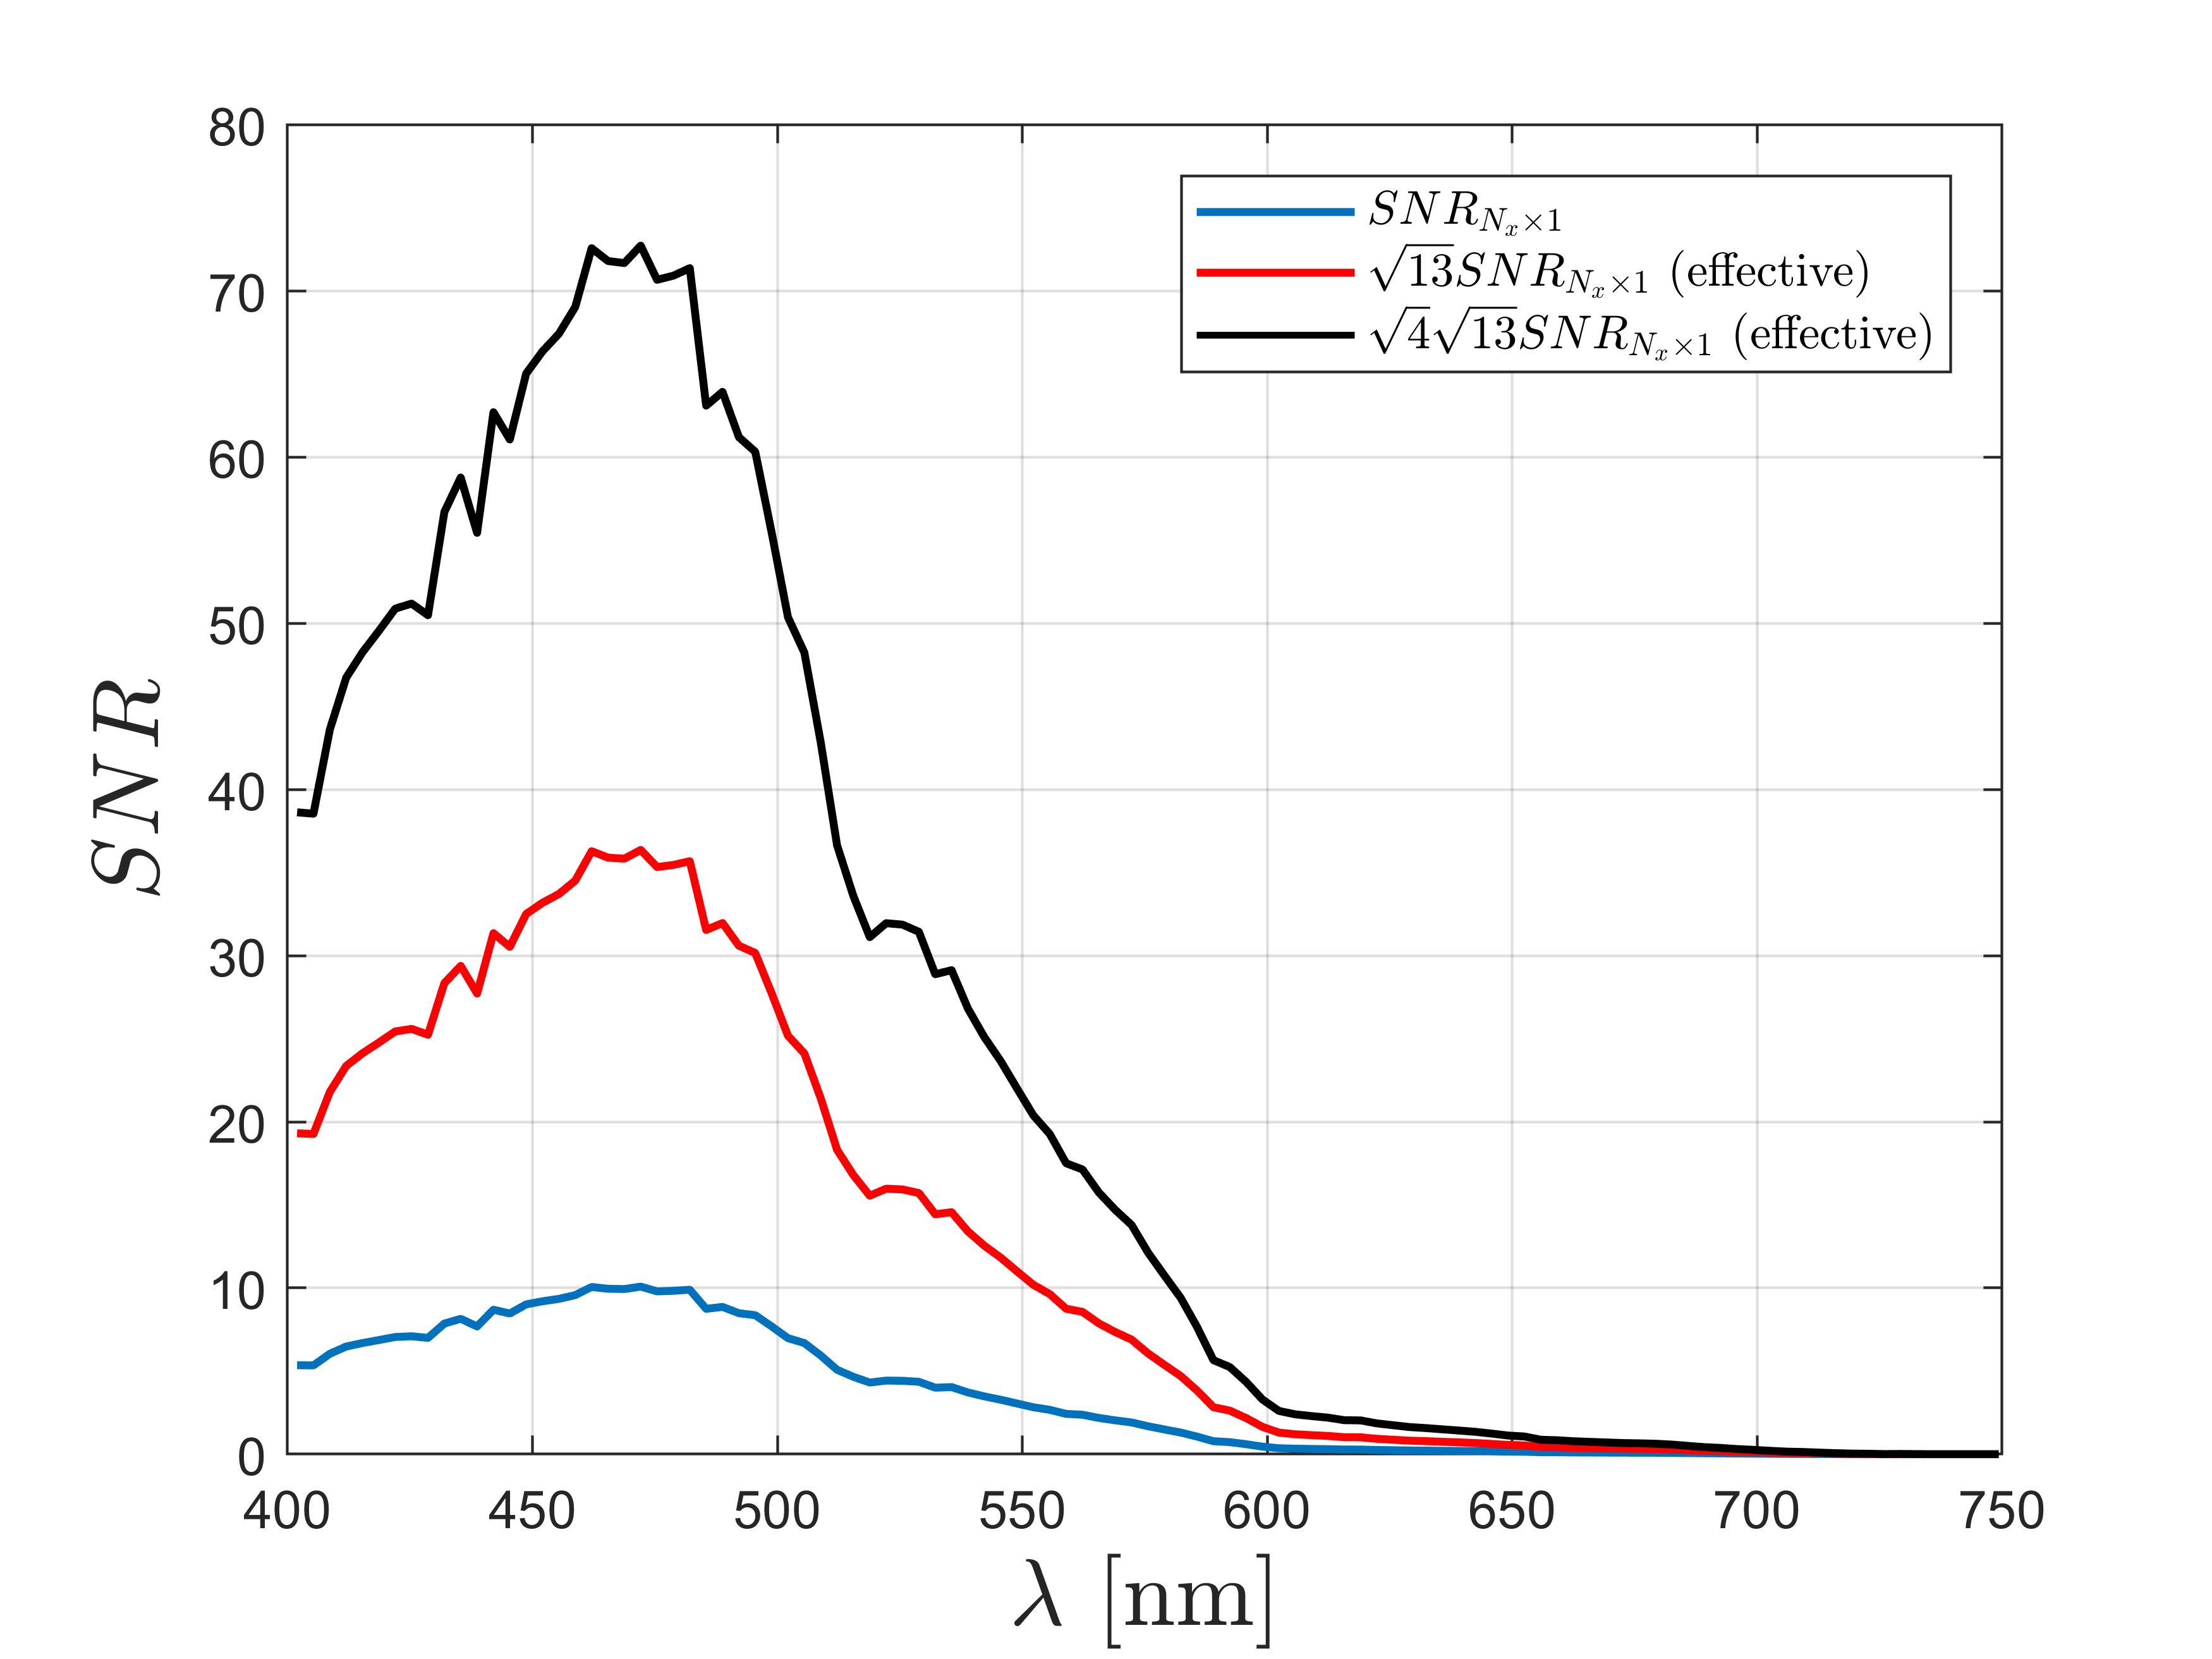
\includegraphics[width=0.45\textwidth]{figs/snr_lambda.png}
%   \caption{SNR in a pixel for a spacecraft HSI sensing the Earth water-leaving radiance $L_w$ at $\gamma=0^{\circ}$. The dashed red curve shows the effective SNR in the case of $13$ overlapping pixels. The dashed black curve shows effective SNR when 4 spacecraft are mapping the same target area with 13 overlapping pixels. Exposure time for all spacecraft are $\tau=25 \hspace{3pt} \rm{ms}$.}
% 	\label{fig:snr_lambda}
% \end{figure}
\section{HYPSO-1} \label{hypso-mission}
% \textcolor{blue}{Contribution (3): "We present the chosen spacecraft bus of HYPSO-1 and justify the feasibility of the concept based on the spacecraft capabilities in terms of its chosen subsystems as well as power, communications and data budget constraints."
% Key points to keep in mind while writing this section are:
% \begin{itemize}
%     \item How will the chosen HYPSO-1 bus (present an overview) enable the CONOPS discussed in section \ref{sec:mission-design}?
%     \item What are the key subsystems that impact the CONOPS discussed in section \ref{sec:mission-design}?
%      \item What are the constraints with using the HSI discussed in section \ref{sec:hsi} (and spacecraft constraints on HSI?)?
%     \item Justify with technical system budgets how the CONOPS is feasible as discussed in section \ref{sec:mission-design}
% \end{itemize}}
\subsection{Spacecraft Bus} \label{sec:spacecraft}
% The mission objectives drive the design of the system, and design decisions must be made at the operational, system, functional, logical and the physical levels. 
% \textcolor{red}{ to provide the capabilities required to satisfy the CONOPS discussed in section \ref{sec:mission-design}. However, the COTS-based design is subject to what is available, and trade-offs must be made in terms of performance and functionality for the system design. .}

% This section will describe the spacecraft and the subsystems selected to support the mission, and discuss the constraints and their impact on the system design and CONOPS.
\begin{figure}[htbp]
  \centering
      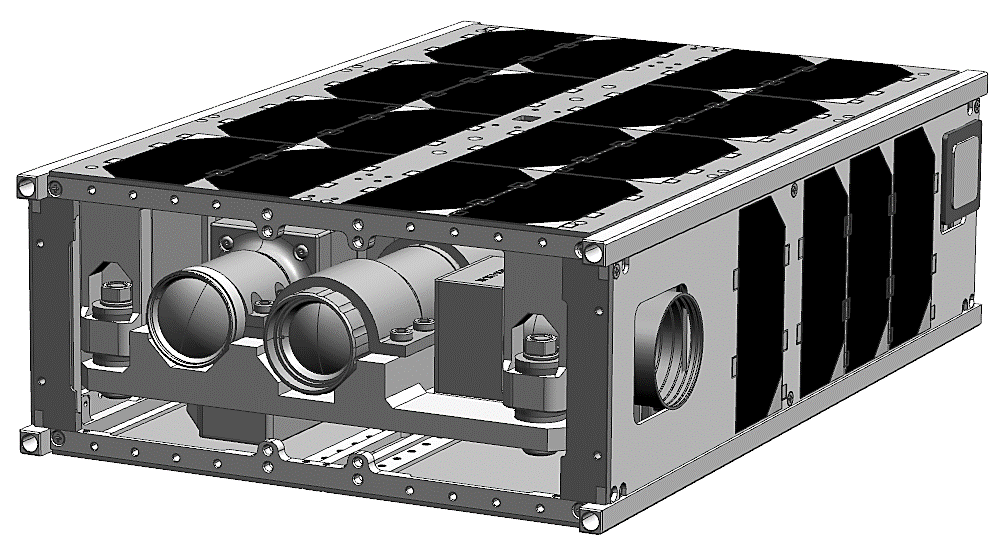
\includegraphics[width=0.4\textwidth]{figs/M6P.png}
  \caption{Isometric view of M6P with front panel removed showing the hyperspectral imager in the center, a RGB camera to its left and a star-tracker to its right.}
\end{figure}
Due to cost, schedule, and resources available, the hyperspectral imager, described in Section \ref{sec:hsi}, was chosen to be integrated to a commercially available spacecraft bus. The chosen bus is the Multipurpose 6U Platform (M6P) provided by NanoAvionics. The hyperspectral imager must adapt to existing bus interfaces which in turn affects the mission operations. Continuous iterations based on discussions with end users affected the mission and systems design concurrently, a common process in spacecraft development \cite{Ryschkewitsch2009,boehm1988,smad1999}. 
% The feasibility of CONOPS, described in section \ref{sec:mission-design}, can be determined by analysis of the power and data latency budgets.

Among the important subsystems of M6P are the Flight Computer (FC) for onboard data handling and ADCS functions, a SatLab Global Navigation Satellite System (GNSS) for accurate positioning and on-board time synchronization through a Pulse-per-Second (PPS) signal, Electrical Power System (EPS) for power management, a UHF Radio for basic communications, and a Payload Controller (PC) working as a network interface and router between the payload and the bus. All subsystems communicate over a CubeSat Space Protocol (CSP) and Controller Area Network (CAN) network, where each subsystem is a node with its own CSP address. To fulfill the CONOPS described in Section \ref{sec:mission-design}, the M6P is tailored to be equipped with: 
\begin{itemize}
    \item 16 triple junction solar cells made of Gallium Arsenide that charge six Lithium-Ion batteries with a combined energy capacity of approximately $64.9 \hspace{3pt} \rm{Wh}$, providing enough power for the planned sequences.
    \item A BICE NST-1B star-tracker with FoV of $21^{\circ}$ and measuring accuracy of $8 \hspace{3pt} \rm{arcsec}$ along the $x_b$ and $y_b$ axes and STIM 210 IMU with bias stability of $1.32\times 10^{-6}\rm{deg/s}$ and noise standard deviation of $8\times 10^{-3} \rm{deg/s}$, which are dedicated for the slew maneuver to provide precise attitude accuracy. To ensure sufficient settling time in the sensors' temperature-dependent bias and initialization in the attitude estimator algorithm, the sensors are turned on for at least $4 \hspace{3pt} \rm{min}$ prior imaging. Since the sensors consume a lot of power they are therefore scheduled to immediately turn off when the slew maneuver is complete. For operations without hyperspectral imaging, the M6P's six sun sensors, three magnetometers and three Micro-Electro-Mechanical-System (MEMS) gyroscopes are used instead when provide coarser attitude determination to relieve the power budget. 
    \item Four reaction wheels are used for attitude control and provide up to $3.2 \hspace{3pt} \rm{mNm}$ torque each, three being placed orthogonal to each other and the fourth at a $54.7^{\circ}$ angle with respect to the other three. 
    % Two magnetorquers, that may produce a maximum magnetic dipole of $0.46 \hspace{3pt} \rm{Am^2}$ each, are placed along each body axis and are used for reaction wheel momentum dumping.
    \item A RGB camera (IDS UI-125x, 6mm, f/1.4 Ci Series Fixed lens, with custom housing) that takes images with a footprint of $770 \hspace{3pt} \rm{km} \times 540 \hspace{3pt} \rm{km}$ and spatial resolution of approximately $500 \hspace{3pt} \rm{m}$, whose main purpose is to support and validate the orthorectification of hyperspectral images in the spatial domain \cite{habib2016ortho}.
    \item A $2.4 \hspace{3pt}  \rm{GHz}$ Satlab S-band Transceiver provides an usable data rate of up to $1 \hspace{3pt} \rm{Mbps}$ for downlink of payload data to the ground. 
    \item An Onboard Processing Unit (OPU) which is dedicated to fast image processing of hyperspectral data. It based on a Xilinx PicoZed SoC that consists of two core ARM processors and a Field Programmable Gate Array (FPGA). The FPGA enables reconfiguration of hardware for specific applications after launch. The PicoZed interfaces with the RGB and hyperspectral cameras through a customized breakoutboard. Large amounts of payload data need to be transferred from the OPU to the PC at a usable CAN speed of $0.4 \hspace{3pt} \rm{Mbps}$ before transmitting over the radio. It also hosts two SD-cards that allows storing up to $24 \hspace{3pt} \rm{GB}$ of data. 
\end{itemize}

\subsection{Power Budget}
Given that HYPSO-1 is in a $500 \hspace{3pt} \rm{km}$ SSO with Right Ascension of Ascending Node of $198.42^{\circ}$, the comprehensive results for the power budget are shown in Tables \ref{tab:power-budget}. The orbit is shown in Figure \ref{fig:orbit_hypso}.
\begin{figure}[tbhp]
  \begin{center}
    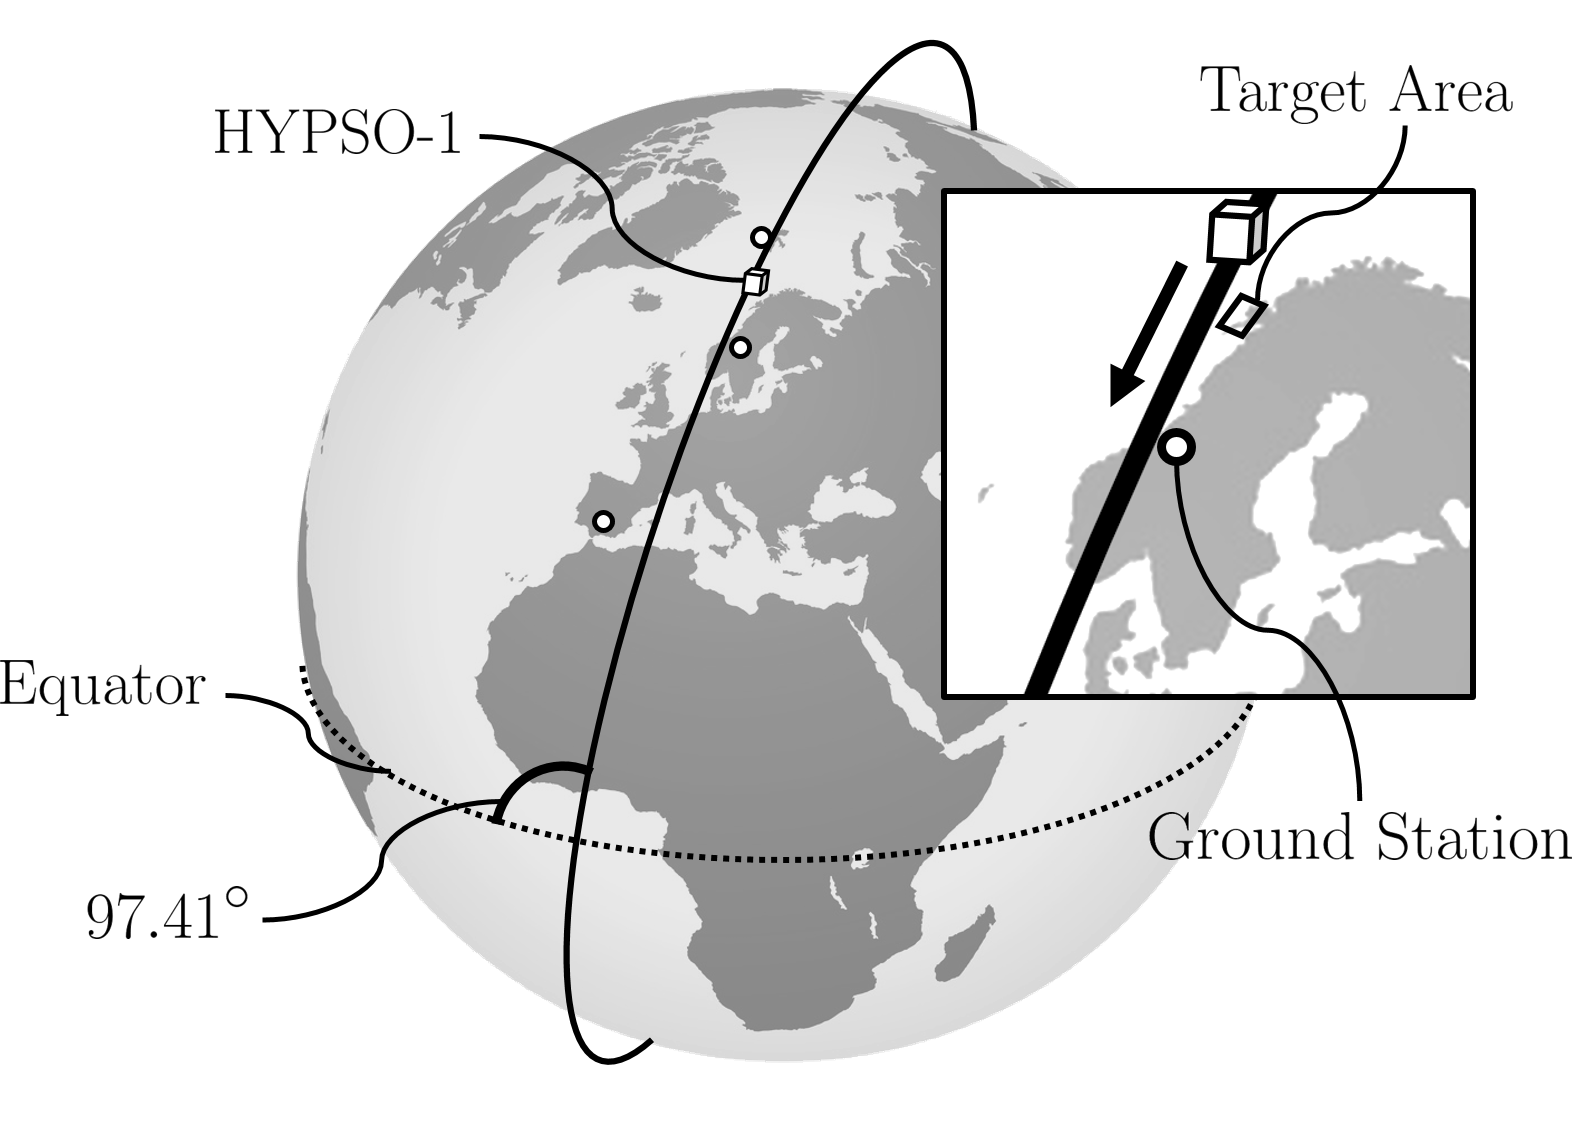
\includegraphics[width=85mm,angle=0]{figs/orbit_hypso.png}
    \caption{The orbit of HYPSO-1 at 10:14:15 on 19 August 2021. The target area is Lofoten, Norway. Selected ground stations at NTNU, KSAT Svalbard and KSAT Spain are represented by white circles.}
    \label{fig:orbit_hypso}
\end{center}
\end{figure}
\begin{table}[htbp]
	\caption{Power budget}
	\label{tab:power-budget}
	\centering
			\begin{tabular}{l r r r}
				\hline
				Battery Capacity & $64.90 \hspace{3pt} \rm{Wh}$ & & \\ 
				Generated Power & $11.65 \hspace{3pt} \rm{W}$ & & \\ 
			   Efficiency & $84.64 \hspace{3pt} \rm{\%}$ & & \\
			   \hline
			  Subsystem & Power ($\rm{W}$) & DC ($\%$) & Power Used ($\rm{W}$) \\
			  \hline
				Hyperspectral imager & 3.675 & 1.054 & 0.039 \\
				RGB camera & 3.360 & 0.019 & $6.384\times10^{-5}$ \\
				OPU imaging & 3.059 & 1.054 & 0.003 \\
			    OPU image processing & 2.315 & 4.76 & 0.146 \\
			    OPU CAN transfer & 2.132 & 35.33 & 0.753 \\
				ADCS normal & 4.765 & 94.77 & 4.516 \\
				ADCS precise & 7.907 & 5.23 & 0.414 \\
			    S-band radio RX & 4.813 & 10.57 & 0.509 \\
				S-band radio TX+RX & 12.201 & 10.57 & 1.290 \\
				Other & 1.153 & 100 & 1.153 \\
				\hline
				Total ($+10\%$ margin) &  & & 9.706 \\
				Remaining &  & & 0.155 \\
				\hline
				\end{tabular}
\end{table}

The M6P solar arrays are able to generate approximately $11.65 \hspace{3pt} \rm{W}$ during $3532 \hspace{3pt} \rm{s}$ out of the total orbit period of $5677 \hspace{3pt} \rm{s}$ (accounting for $2145 \hspace{3pt} \rm{s}$ time in eclipse). It is assumed that the input and output efficiencies of the batteries are $92 \%$ each. Table \ref{tab:power-budget} shows the physically measured nominal power ratings with $5 \%$ component margin and corresponding duty cycles (DC). The OPU, ADCS and S-band radio power ratings are distinguished into more than one operational mode, while "Other" denotes the collective power consumption by FC, EPS, PC and internal bus communications. In particular, high power consumption is expected during the HSI image acquisition and slew maneuver when the IMU and star-tracker are active, consuming up to $1.5 \hspace{3pt} \rm{W}$ each. Adding a $10 \%$ system margin results in remaining available power of about $0.155 \hspace{3pt} \rm{W}$. Constrained by the power budget, allowed downlink time is $10 \hspace{3pt} \rm{min}$ per orbit which means that potentially $75 \hspace{3pt} \rm{MB}$ of data may be downloaded. The allowed for transferring data through CAN is set to $33.42 \hspace{3pt} \rm{min}$ while the time for OPU on-board image processing can be set at a maximum of $270 \hspace{3pt} \rm{s}$.
% As the mission matures other parts of the processing pipeline can become a a part of the on-board processing and then the reconfigurability of the FPGA is a crucial feature to achieve the desired performance when dealing with gigabytes of hyperspectral data.
% \subsubsection{Communications}
% \hl{Roger \\}
% The satellite bus is equipped with two independent communication systems; one Ultra High Frequency (UHF) transceiver and one S-band transceiver. All subsystems can be reached through both radios thanks to the on-board CubeSat Space Protocol (CSP) network. The UHF radio is practical for preparing a high-level telemetry beacon, and giving access to basic telecommands. The S-band radio is primary used for payload data and for software updates. 

% UHF was chosen for ease of operations, especially during commissioning, and S-band was chosen because of the ground segment availability, both commercial and institutional. There was also a large range of S-band subsystems available at a reasonable cos when the subsystem had to be  selected. This gives the highest download rates with largest ground segment availability. X-band was considered but rejected due to a much higher cost. The payload generates a vast amount of data during high resolution imaging, and the radio will be a bottleneck for data downloading. Compression of acquired data will improve this, and reduce the time and energy needed for downloading. 
% \subsubsection{RGB Camera}
% \hl{Joe, Sivert \\}
% The HSI pushbroom camera will be augmented by an RGB camera (IDS UI-125x, 6mm, f/1.4 Ci Series Fixed lens, with custom housing) that takes regular spatial images. 
% The RGB camera will be able to cover an area on ground of 770 $\times$ 540 $km^2$, with a spatial resolution of just under 500 m. 
% Images from the RGB camera will be used as an aid for and as validation of the orthorectification \cite{habib2016ortho} that will be performed to get spatially coherent HSI images.

% In addition to this, the RGB images can be used for pan-sharpening \cite{loncan2015pansharpening}, a technique that would increase the overall spatial resolution of the HSI cubes by inferring spectral values into the higher sampled spatial domain from the RGB images.

% \subsubsection{On-board Processing Unit}
% \hl{Joe, Sivert \\}
% The Onboard Processing Unit (OPU) is based on a Xilinx PicoZed SoC that consists of an ARM processor and a Field Programmable Gate Array (FPGA). 
% The FPGA is a semiconductor device that enables development of features and functions, as well as reconfiguration of hardware for specific applications after launch.
% The PicoZed interfaces with the RGB and HSI cameras through a customized breakoutboard. 
% The two cameras contain firmware to facilitate in image capture and so they are also part of OPU. The OPU is connected to the other satellite subsystems utilizing the CAN network. 

% The OPU will facilitate on-board processing of the hyperspectral data. 
% At the time for launch, the OPU will enable lossless compression by the CCSDS123v1 algorithm\cite{Fjeldtvedt2018}, reducing the HSI image cube size by a factor of 2.5 or more, and making it possible to run such algorithms as part of the on-board processing.
% The purpose of the on-board processing is to enable the pertinent information to be extracted from the hyperspectral images and downlinked within a few passes.

% As the mission matures other parts of the processing pipeline can become a a part of the on-board processing and then the reconfigurability of the FPGA is a crucial feature to achieve the desired performance when dealing with gigabytes of hyperspectral data.
% \subsubsection{Other subsystems}
% \hl{Evelyn, Roger, Mariusz \\}


% The EPS includes \hl{X} number of batteries with \hl{X} $\rm{Wh}$ capacity and has five modes: Full Mode, Normal Mode, Safe Mode, Critical Mode and Hardware Critical Mode, where the subsystem states can be configured to be on or off. The voltage thresholds on triggering the modes are configurable.

%Suggestion


% \subsection{Ground Station Network (Ground Segment)}
% \hl{Roger, Mariusz, Joe \\}
% TO BE MOVED TO CONOPS
% %Only discuss Ground stations... 
% % \begin{figure}[tbhp]
% %   \begin{center}
% %     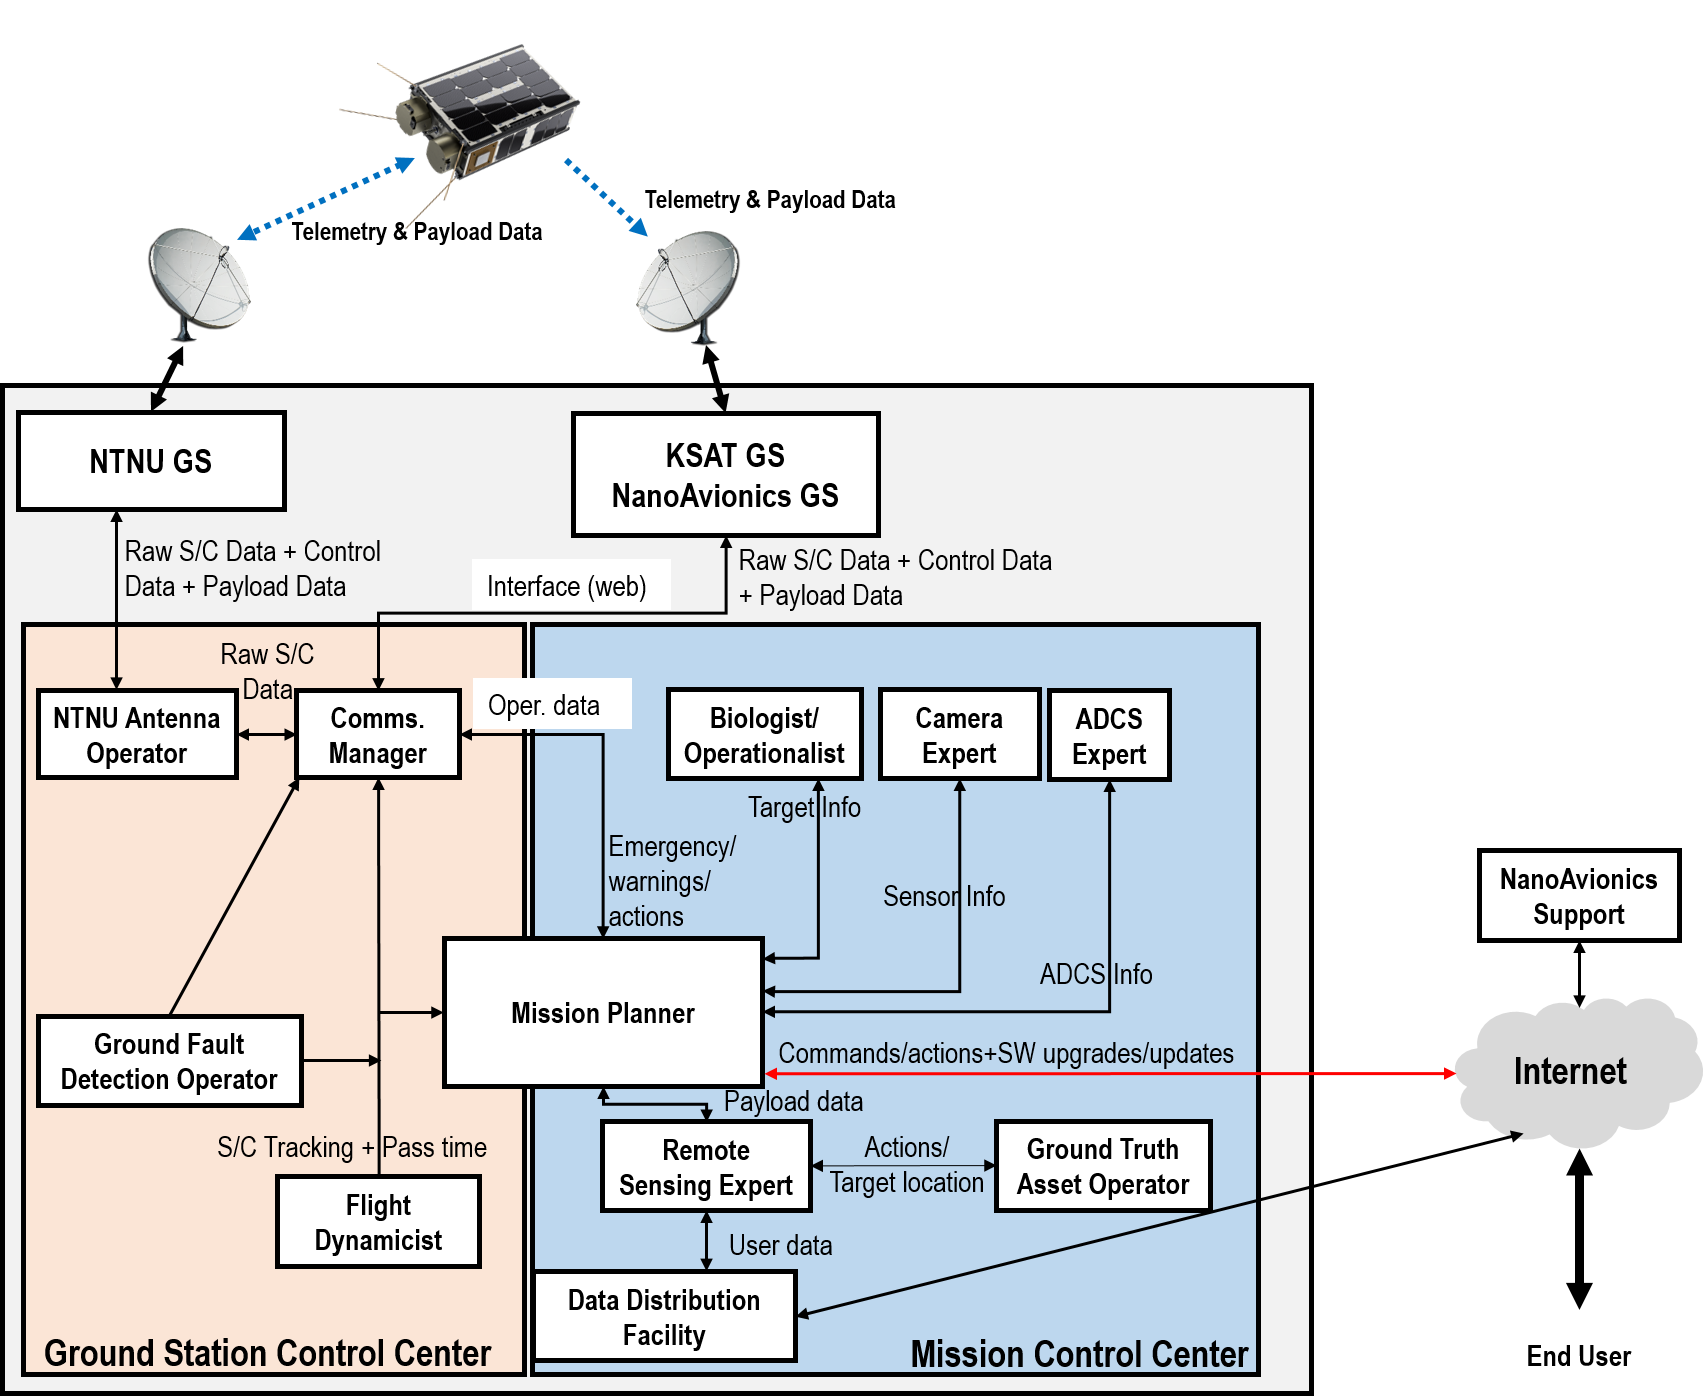
\includegraphics[width=80mm,angle=0]{figs/HYPSO_GS.png}
% %     \caption{HYPSO Ground Segment Architecture.}
% %     \label{fig:hypso-GS}
% % \end{center}
% % \end{figure}

% In order to facilitate the agility needed for mission operations, the system must make use of ground station gateways (GWS) at different locations to reduce the communication revisit time. The mission operations center (MOC) will be located at NTNU, co-located with one combined S-band and one UHF station. Other S-band stations are available through the KSAT Lite network, as well as through NanoAvionics and partners. 

% The use of the GWS is coordinated by the mission control software (MCS, NanoAvionics). This software acts as a router between the MOC, GWSs and the satellite. The MCS will route data intended for the satellite through the correct GWS during a pass. Data from the satellite is likewise routed from through the GWS and MCS to the end user. 
% \begin{figure*}
%     \centering
%     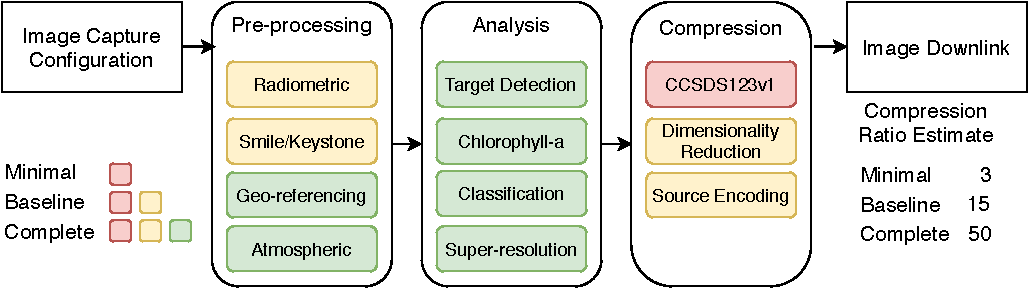
\includegraphics[width = 0.9\textwidth]{figs/img_processing/pipeline_figure_concept_paper.pdf}
%     \caption{Illustration of proposed imaging pipelines. Minimal for launch, baseline for the first updates, and complete when reached maturity.}
%     \label{fig:image-processing-pipelines}
% \end{figure*}

\begin{figure*}
    \centering
    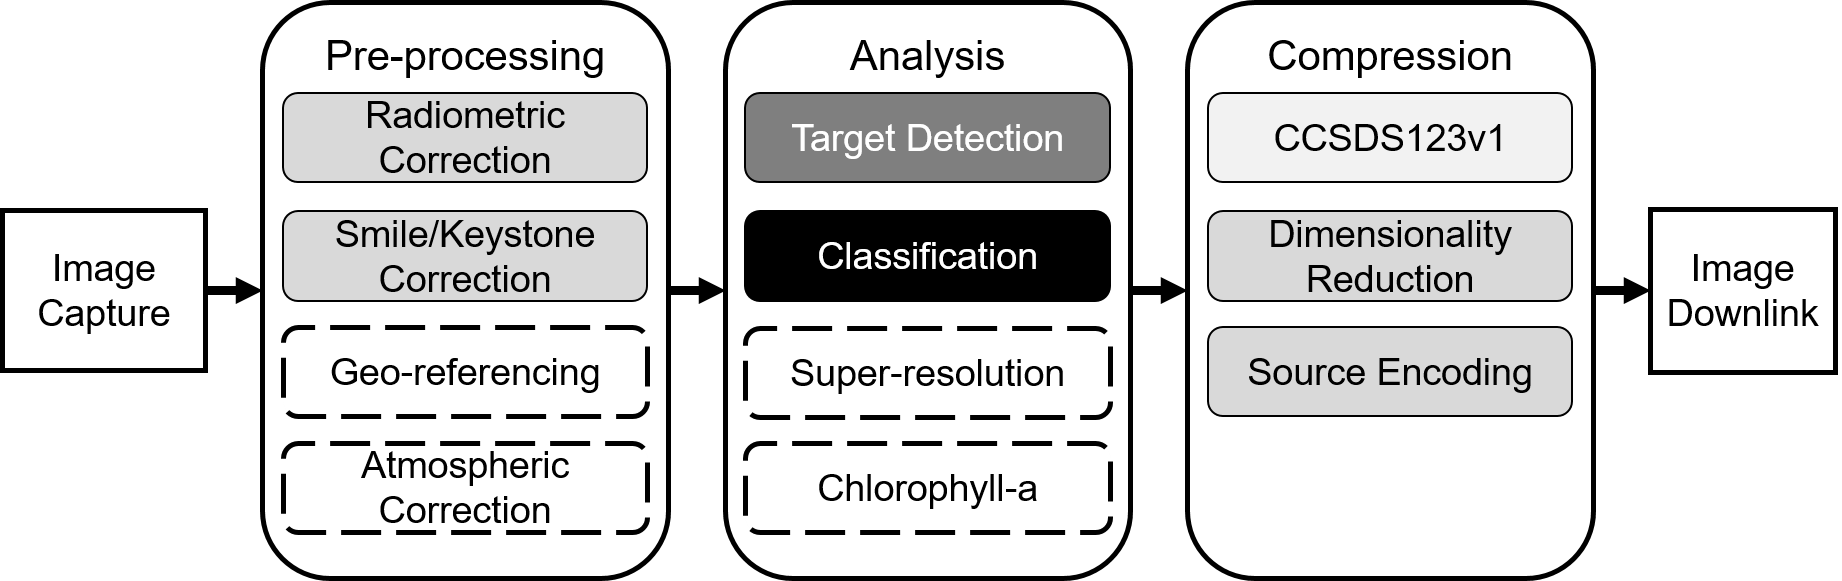
\includegraphics[width = 0.8\textwidth]{figs/img_processing/image-processing-pipeline.png}
    \caption{Diagram of the proposed imaging processing pipelines. Lightest gray block represents MOBIP, darker gray blocks represent BOBIP, darkest gray block represents TOBIP and black block represents COBIP. The dashed blocks represent modules planned for advanced image processing pipelines.}
    \label{fig:image-processing-pipelines}
\end{figure*}
\subsection{Image processing architecture}
 Figure \ref{fig:image-processing-pipelines} illustrates a diagram of the HYPSO-1's modular image processing architecture which is implemented on the OPU. 
% The modular design allows the operators to switch between the modules as needed. 
The modules can be arranged flexibly with specific orderings that each generate tailored data products, designated as image processing pipelines.
% Binning and subsampling is incorporated into the imager configuration itself to enable higher FPS with lower data traffic and so the most raw data is reduced before the image processing pipelines begin.
The estimated data size reduction factors for each pipeline are shown in Table \ref{tab:data-reduction}.
\begin{table}[htbp]
	\caption{Estimated Data Reduction of Image Processing Pipelines}
	\label{tab:data-reduction}
	\centering
	\begin{tabular}{l |r}
	\hline
	Pipeline & Factor \\
	\hline
    Minimal On-Board Image Processing (MOBIP) & 3 \\
    Baseline On-Board Image Processing (BOBIP) & 14.8 \\
    Target Detection On-Board Image Processing (TOBIP) & 49.9 \\
    Classification On-Board Image Processing (COBIP) & 93.2 \\
    \hline
\end{tabular}
\end{table}
% The planned on-board processing is divided into multiple different pipelines, illustrated in figure \ref{fig:image-processing-pipelines}, that share a basic structure, i.e. some level of processing has to be performed regardless, while others may only improve the timeliness of desired data products or reduce the expected data volume to be down-linked. In the subsequent section a high-level description of the software used and planned in the on-board processing is provided.
% \subsubsection{Settings \& Pre-processing}
% The HSI camera will collect spectrograms at a rate of 15-40 Hz. 
% The data rate is limited by the GigE that connects the camera to the breakout board, but by reducing the area of interest or doing sub-sampling in the spectral dimension, the rate at which frames are collected is adjusted \cite{varntresk2019assembly}. 
% It is expected that the imaging sensor of the HSI camera will have some distortions as a result of the optics, and that the sensitivity of given pixels will change over time. 
% Pre-processing, the initial stage of the imaging pipeline seeks to accommodate these undesirable artifacts.
\begin{table*}[htbp]
	\caption{Uncompressed Data Products*} %\textcolor{red}{Update this Re. Table VI}}
	\label{tab:data-products}
	\centering
	\begin{tabular}{l | r r r r}
	\hline
	& Bands & Pixel size ($\rm{bits}$) & Signatures ($\rm{MB}$) & Total ($\rm{MB}$) \\
	\hline
	Raw & 1074 & $16$& - & 1716 \\
	Binned & 119 & $16$ & - & 190.1 \\
	Dimensionality reduced & 20 & $16$ & - & 32.0 \\
	Classification (16 classes) & 1 & $4$ & 0.003 & 0.40 \\
	Classification (256 classes) & 1 & $8$ & 0.051 & 0.85 \\
	Target detection (only ACE) & 1 & $16$ & - & 1.60\\
	Target detection (with abundance) & 2 & $16$ & - & 3.20 \\
	Target coordinates (top 100) & n/a & $16$ & - & 0.001 \\
	\hline
	\end{tabular}
	
	\begin{tabular}{c}
		*assuming 1168$\times$684 spatial pixels. %\hl{what about spatial compression - jpeg?}
	\end{tabular}
	\vspace*{-\baselineskip}

\end{table*}
\subsubsection{Minimal on-board image processing}
The minimal on-board image processing (MOBIP) pipeline consists of the CCSDS123v1 lossless compression algorithm which is implemented on the OPU's FPGA but can also run on the CPU \cite{Fjeldtvedt2018, orlandic_parallel_2019}. The data size is reduced by a factor of approximately 3. Without loss of spatial or spectral information, the MOBIP data product can be provided to end users who wish to process the data further.  

\subsubsection{Baseline on-board image processing}
The baseline on-board image processing (BOBIP) pipeline adds two important modules to MOBIP, before source encoding and compression are applied. 
The first is a smile and keystone correction, which adjusts images to account for systematic optical and measurement errors inherent to the imager \cite{Henriksen2019}. 

Second is dimensionality reduction, which allows for control of data size while retaining most of the information of the image by adjusting the number of selected reducted bands. \cite{Vit17}. 
% \hl{removing noise-like and redundant components }. 
The smile and keystone correction is applied before the dimensionality reduction to prevent the latter from intertwining systematic, but reversible artifacts irrevocably with the data. For image processing modules beyond BOBIP, dimensionality reduction will increase the computational speed because there will be fewer bands to process \cite{Bakken2019SPIE}.

% \textcolor{red}{For BOBIP, the On-the-Fly-Processing (OTFP) algorithm cam be used as dimensionality reduction because it allows for accurate reconstruction of the hypserspectral information with a minimal number of bands \cite{Vit17}. 
% The residuals from the dimensionality reduction can also be downlinked occasionally and analysed to provide insight about the components removed from the data.
% Once it is rigorously tested and approved, the BOBIP pipeline will provide the nominal data products. 
% For BOBIP the number of selected bands is expected to be about 20.

\subsubsection{Target detection on-board image processing}
Another way to expand MOBIP or BOBIP is to add a target detection (TD) module before compression, named target detection on-board processing (TOBIP) pipeline. Hyperspectral data is amenable to target detection because of its numerous channels \cite{Manolakis2002, Manolakis2005}. One target signature will result in a probability map, or a heat map, of its occurrence across the scene. Multiple target signatures can be represented as separate bands. 
% By incorporating spectral information about the background scene, TD algorithms can locate sub-pixel spectral signatures.
% The 2D heat maps produced by TD are small in data size and can be immediately used to guide in-situ agents without requiring additional processing on ground. 
The Adaptive Cosine Estimator (ACE) is a target detection algorithm for hyperspectral images that is often used to determine the likelihood of a pixel containing a particular spectral signature. 
Both software and software-hardware co-design versions of the algorithm have been developed for OPU. Computing acceleration provided by the OPU's FPGA results in a speedup factor of about $28$ times relative to software implementations \cite{dijehw19_meco}. Effective use of ACE requires a-priori knowledge about the target spectra to be observed. 
% \textcolor{orange}{A spectrum can either be estimated from data in the lab, which is susceptible to calibration inconsistencies between the lab camera and the satellite camera, or it can be estimated directly from the satellite data, so that the target spectrum and input data traverse similar optical paths \hl{?}}. 
A complementary algorithm, the abundance estimator, can be used to estimate how much of a pixel is contained by a target signature. 
For some applications, such as chlorophyll estimation, the abundance estimator itself will be the most relevant component of the data. 

The maxima in a heat map show the pixel locations where it is most probable that a particular target signature is present. Instead of downlinking the entire heat map it is possible transfer only the pixel coordinates of a number of the maxima. If the coordinates are geo-referenced, the in-situ agents can quickly travel to the location of these maxima to inspect in more detail. For example, if the location of the 100 largest local maxima of the map are downlinked together with their latitudes and longitudes, the total data package will only be about $1 \hspace{3pt} \rm{kB}$, shown in Table \ref{tab:data-products}. % The small size of this data product can be quickly downlinked after image acquisition, and for that reason it will enhance the capability of in-situ agents to track dynamic ocean phenomena.
\subsubsection{Classification on-board image processing}
Alternative to TOBIP is the classification on-board image processing (COBIP) pipeline with a classification algorithm that separates the pixels of a hyperspectral image into different classes \cite{Alcolea_2020}. With fewer than 16 classes, it is possible to represent each pixel with a 4 bit integer whereas up to 256 classes can be represented with 8 bits. Representative spectra for each class will also be downlinked. 

Graph-based clustering, an unsupervised method, will be adapted to be run on the OPU as the initial classification algorithm because of its flexibility and it does not require training data \cite{Wang2017}.
Once a database of hyperspectral images is acquired and labelled, a supervised classification algorithm will be incorporated as an alternative.
Recent experiments have shown that gradient boosting decision trees achieve a good balance of accuracy and computational requirements for on-board processing \cite{Alcolea_2020}.
\subsection{Advanced on-board image processing pipelines}
Additional planned algorithms, some of them depicted in dashed blocks in Figure \ref{fig:image-processing-pipelines}, are still in development and may be uploaded on the OPU while HYPSO-1 is in orbit and implemented in a similar successive mission. 
The planned algorithms include image registration, motion-blur correction, geo-referencing, atmospheric correction, and super-resolution, some of them slated to be run on ground. 
% Several of these kinds of algorithms utilize the RGB camera in addition to the hyperspectral imager, so it must be drawn into the image processing pipelines. 
Depending on the end user and target area, different tailored data products will be desired and more modules can be added to the image processing architecture based on these needs. We discuss a few selected algorithms next.

\subsubsection{Image registration and geo-referencing}
In general, even very simple algorithms for registration and geo-referencing require more computational power than is available on-board the HYPSO-1 \cite{Opsahl_2011}. Here, we refer to image registration as the determination of the relative separation of the individual pixels, or sometimes named orthorectification, and geo-referencing as the process of assigning all the pixels to latitude and longitude coordinates. For example, registration is necessary to enable any spatial-spectral methods in image classification, which tend to be more accurate than those that rely only on spectral information. Similarly, to downlink the target detection local maxima coordinates, it is necessary to determine what the latitude and longitude of the relevant pixels. For on-board operation, a simple ray-tracing method will be adapted, which has been prototyped on the ground for joint registration and geo-referencing, similar to the one described in \cite{Schlapfer2002} but with a flat elevation model for the water surface. 
% However, it is expected that more advanced perturbative techniques may be required, and those techniques will initially be run on the ground. 

\subsubsection{Super-resolution}
Super-resolution algorithms are being adapted to enhance the spatial resolution in the images as described in \cite{Park2003}, and may provide high-accuracy and resolution. The initial prototypes for super-resolution model require a measurement process, e.g. determining the point-spread function, and then use that to infer the image at higher spatial resolution \cite{Garrett2019}. The prototypes are based on methods that come from multi-frame super-resolution because of its similarity with the irregularly-sampled data from the slew maneuver \cite{stark_high-resolution_1989, farsiu_fast_2004}. 
Although these super-resolution algorithms do improve the resolution somewhat, they are susceptible to noise, digitization, compression and inaccuracies in the estimate of the point spread function \cite{Baker2002,Kohler2019}. 
However, some of these measurement-based super-resolution methods have previously been successfully applied to remote sensing data \cite{clarisse2019tracking}. 

Prior-based super-resolution techniques overcome the limitations of measurement-based reconstruction techniques by supplementing the input pixels with additional expectations about image statistics. 
Examples of general prior-based techniques include sparse image representations \cite{Yang2010}, and convolutional neural nets \cite{Kim_2016_CVPR,Anwar2020}. 
Some of these produce plausible images at magnification factors of up to 8 times, and even a factor of 6 times. However, these techniques are specifically designed for hyperspectral data. 

On the other hand, dimensionality reduction-based super-resolution techniques unique to hyperspectral imagery have been developed as well \cite{Akgun2005}. Recently, numerous multispectral-hyperspectral fusion techniques have been proposed to enhance the resolution of the latter \cite{Lanaras_2015_ICCV, Yokoya2017}. For utilizing super-resolution in the HYPSO-1 mission, it is necessary to determine how it can be incorporated into a framework with classification or target detection.

\subsubsection{Upload/reprogram Capability}
Both the software and FPGA configurations are planned to be updated during the operation of the satellite \cite{Gjersund2020}. 
The software update must be stringently tested on the ground, both in terms of timeliness and computing resources, before uploading it which can take several passes to complete. 
The OPU retains \textit{golden image}, a version of the operating system and software known to have worked, that it will revert to in case of an update failure. 

\subsubsection{Ground Processing Pipeline}
Similar and extended image processing pipelines should operate on the ground to (a) adjust, fine-tune and prepare data for end users; (b) assist in in-orbit calibration of the hyperspectral imager; and (c) to test algorithms rigorously before uploading them to the satellite for on-board image processing. 
Some of the components of the pipeline such as geo-referencing, atmospheric correction and super-resolution are also amenable to being applied to the data on ground because they require access to reference libraries and are more computationally expensive than the other modules presented.
% \begin{table}[htbp]
% 	\caption{Data budget}
% 	\label{tab:data-budget}
% 	\centering
% 			\begin{tabular}{l r r r r}
% 				\hline
% 				S-band TX Data Rate & $1 \hspace{3pt} \rm{Mbps}$ & & & \\ 
% 				S-band RX Data Rate & $0.04 \hspace{3pt} \rm{Mbps}$ & & & \\ 
% 			   CAN Buffer Speed & $0.4 \hspace{3pt} \rm{Mbps}$ & & & \\
% 			   \hline
% 			    & Upload & TM & Data A & Data B \\
% 			  \hline
% 		    Data Size (MB) & 0.1 & 0.1 & 100.29 & 11.06 \\
% 			CAN Transfer Time (min) & 0.03  & 0.03 & 33.43 & 3.69 \\
% 			Downlink Time (min) & - & 0.01 & 13.37 & 1.47 \\
% 		    Uplink Time (min) & 0.33 & - & - & -  \\
% 		    Orbits Required & 0.0039 & 0.0021 & 2.58 & 0.08 \\
% 				\hline
% 				\end{tabular}
% \end{table}

% \begin{table}[htbp]
% 	\caption{Data Constraints}
% 	\label{tab:data-constraints}
% 	\centering
% 	\begin{tabular}{l r }
%         \hline
%         Available onboard processing time	& $347.26 \hspace{3pt} \rm{s}$\\			
%         Available onboard transfer time &	$2005.80 \hspace{3pt} \rm{s}$\\			
%         Available downlink time &	$1320 \hspace{3pt} \rm{s}$ \\				
%         Maximum data transferred per orbit &	$100.29 \hspace{3pt} \rm{MB}$ \\
%         Total downlink per orbit (incl. headers) &	$165 \hspace{3pt} \rm{MB}$ \\				
%         SD card storage space available	& $24 \hspace{3pt} \rm{GB}$ \\
%         \hline
%     \end{tabular}
% \end{table}
\begin{table*}[htbp]
	\caption{Summary of selected hyperspectral imager mode performance}
	\label{tab:data-types}
	\centering
	\begin{tabular}{l r r r r r}
        Type &	Mode A & Mode B & Mode C & Mode D & Mode E \\ % OK
        \hline
        ADCS Mode &	Slew ($\theta_0=20^{\circ}$) & Slew ($\theta_0=20^{\circ}$) & Slew ($\theta_0=20^{\circ}$) & Nadir & Nadir \\ % OK
        AoI (pixels) &	$1074\times684$ & $1074\times684$ & $1074\times1194$ & $1074\times1194$ & $1936\times1216$\\ % OK
        Binning, $B_\lambda$ (pixels) &	9 & 18 & 9 & 9 & 1 \\ % OK
        % Sub-sampling (pixels) &	1 &	1 &	1 &	1 & 1\\ % OK
        Spectral range ($\rm{nm}$) & $400-800$ & $400-800$ & $400-800$ & $400-800$ & $276-1006$ \\ % OK 
        Spectral bands & 119 & 59 & 119 & 119 & 220 \\ % OK 
        Bandpass ($\rm{nm}$) & 3.33 & 6.67 & 3.33 & 3.33 & 3.33 \\ % OK
        FPS & 22 & 15 & 12 & 12 & 3 \\ % OK
        Exposure time, $\tau$ ($\rm{ms}$) &	41.45 & 49.10 & 49.10 & 49.10 &	49.10 \\ % OK
        Scan duration ($\rm{s}$) & 53.08 & 53.08 & 57.00 & 9.19 & 1.0 \\ % OK
        Number of frames & 1168 & 797 & 685 & 111 & 3 \\
        SNR of target @$471 \hspace{3pt} \rm{nm}$, nadir & 107.87 & 166.52 & 117.75 & 117.75 & 40.00 \\
        Scan distance, along-track ($\rm{km}$) & 40.08 & 40.08 & 69.97 & 69.97 & 7.60  \\ % OK
        Spatial resolution, along-track, nadir ($\rm{m}$) & 542.9 & 550.9 & 573.1 & 873.8 & 873.8  \\
        Swath width, nadir ($\rm{km}$) & 40.08 & 40.08 & 69.97 & 69.97 & 69.97 \\ % OK
        Spatial resolution, cross-track, nadir ($\rm{m}$) & 58.60	& 58.60 & 58.60 & 58.60 & 58.60 \\
        SGSD, along-track ($\rm{m}$) & 47.09 & 69.07 & 124.08 & 634.39 & 2537.56 \\
        Data size, Raw ($\rm{MB}$) & 190.67 & 65.05 & 195.20 & 31.63 & 14.13 \\
        \hline
        Data size, MOBIP ($\rm{MB}$) & 63.56 & 21.68 & 65.07 & 10.54 & 4.71 \\
        Onboard processing time ($\rm{s}$) & 1.64 & 1.22	& 1.65 & 1.11 & 1.05 \\
        CAN transfer time ($\rm{min}$) & 21.19 & 7.23 & 21.69	& 3.51 & 1.57 \\
        Downlink time ($\rm{min}$) & 8.47 & 2.89 &	8.68 &	1.41 & 0.63 \\
        \hline
        Data size, BOBIP ($\rm{MB}$) & 12.82 & 8.82 & 13.12 & 2.13 & 0.51 \\
        Onboard processing time ($\rm{s}$) & 49.30 & 17.48	& 50.45 & 9.01 & 4.58 \\
        CAN transfer time ($\rm{min}$) & 4.27 & 2.94 & 4.37 & 0.71 & 0.17 \\
        Downlink time ($\rm{min}$) & 1.71 & 1.18 & 1.75 & 0.28 & 0.07 \\
        \hline
        Data size, TOBIP ($\rm{MB}$) & 3.82 & 1.30 & 3.91 &	0.63 & 0.28 \\
        Onboard processing time ($\rm{s}$) & 96.97 & 33.74	& 99.25 & 16.92 & 8.11 \\
        CAN transfer time ($\rm{min}$) & 1.27 & 0.43 & 1.30 & 0.21 & 0.09 \\
        Downlink time ($\rm{min}$) & 0.51 & 0.17 & 0.52 & 0.08 & 0.04 \\
        \hline
        Data size, COBIP ($\rm{MB}$) & 2.05 & 0.70 & 2.09 &	0.34 & 0.15 \\
        Onboard processing time ($\rm{s}$) & 96.97 & 33.74	& 99.25 & 16.92 & 8.11 \\
        CAN transfer time ($\rm{min}$) & 0.68 & 0.23 & 0.70 & 0.11 & 0.05 \\
        Downlink time ($\rm{min}$) & 0.27 & 0.09 & 0.28 & 0.05 & 0.02 \\
        \hline
	\end{tabular}
\end{table*}
% \begin{table*}[htbp]
% 	\caption{Data Types}
% 	\label{tab:data-types}
% 	\centering
% 	\begin{tabular}{l r r r r r}
%         \hline
%         Allowed onboard processing time	& $347.26 \hspace{3pt} \rm{s}$ & & & &\\			
%         Allowed onboard transfer time &	$2005.80 \hspace{3pt} \rm{s}$ & & & &\\			
%         Allowed downlink time &	$1320 \hspace{3pt} \rm{s}$ & & & &\\				
%         Allowed data size to transfer per orbit &	$100.29 \hspace{3pt} \rm{MB}$ & & & &\\
%         Allowed to downlink per orbit &	$165 \hspace{3pt} \rm{MB}$ & & & &\\				
%         Allowed to store (SD card)	& $24 \hspace{3pt} \rm{GB}$ & & & &\\					
%         \hline
%         Type &	Data A &	Data B &	Data C &	Data D &	Data E \\
%         \hline
%         ADCS Mode &	Slew &	Slew &	Nadir &	Slew &	Slew \\
%         AoI (pixels) &	$1200\times720$ &	$1200\times720$ &	$1200\times720$ &	? &	?\\
%         FPS &	20 &	20 &	30 &	20 &	20\\
%         Maximum exposure, $\tau$ ($\rm{ms}$) &	50 &	50 &	33 &	50 &	50\\
%         Binning, $B_\lambda$ (pixels) &	3 &	3 &	3 &	? &	12 \\
%         Sub-sampling (pixels) &	4 &	4 &	4 &	? &	1 \\
%         Spectral Bands &	161 &	20 &	161 &	161 &	161 \\
%         Number of frames &	1139 &	1139 &	276 &	1139 &	1139 \\
%         \hline
%         Level 1 data size ($\rm{MB}$) (1/2) &	87.21 &	19.234 &	25.07 &	? &	? \\
%         Time required to transfer ($\rm{min}$)	& 29.07 &	6.4113 &	8.3567 & & \\		
%         Time required to download ($\rm{min}$)	& 11.628 &	2.5645 &	3.34 & & \\		
%         Number of datacubes per orbit &	1.89 & & & & \\				
%         \hline
%         Level 2 data size ($\rm{MB}$) (1/2) &	43.605 & 	9.617 &	12.535 & & \\		
%         Time required to transfer ($\rm{min}$)	& 14.535 &	3.2057 &	4.1783 & & \\		
%         Time required to download ($\rm{min}$)	& 5.814	& 1.2823 &	1.6713 & & \\		
%         Number of datacubes per orbit & & & & & \\					
%         \hline
%         Level 3 data size ($\rm{MB}$) (1/10) &	4.3605 & 0.962 &	1.2535 & & \\		
%         Time required to transfer ($\rm{min}$) &	1.4535 &	0.3207 &	0.4178 & & \\		
%         Time required to download ($\rm{min}$) &	0.5814 &	0.171 &	0.1671 & & \\		
%         Number of datacubes per orbit &	17 & & & & \\ 
%         \hline
% 	\end{tabular}
% \end{table*}

% \begin{table*}[htbp]
% 	\caption{Latency for Mode A Data}
% 	\label{tab:scenario-2b}
% 	\centering
% 	\begin{tabular}{l l l r}
%         \hline
%         Sequence & Start time & End time & Duration ($\rm{s}$) \\	
%         \hline
%         Orbit 1 & & & \\
%         \hline
%     	HSI scan & 10:11:17.00 & 10:12:10.36 & 53.36 \\
%     	Onboard Processing & 10:12:10.36 & 10:12:12.04 &  1.68 \\
%     	CAN Transfer & 10:12:12.04 & 10:34:58.06 & 1366.02 \\
%         Cruise & 10:34:58.06 & 10:52:18.36 & 1040.30 \\
%         Eclipse & 10:52:18.36 & 11:27:10.34 & 2091.98 \\
%         \hline
%         Orbit 2 & & & \\
%         \hline
%         Exit Eclipse & 11:27:10.30 &	11:39:51.17 & 760.87 \\
%         Downlink to KSAT Svalbard & 11:39:51.17 & 11:43:52.46 & 241.29 \\
%         Downlink to NTNU & 11:43:52.46	& 11:48:57.57 & 305.11 \\
%         \hline
%         Total latency ($\rm{hrs}$) & & & 1.63 \\
%         \hline
%     \end{tabular}
% \end{table*}
\begin{table*}[htbp]
	\caption{Latency for Mode A data}
	\label{tab:scenario-2b}
	\centering
	\begin{tabular}{l | l r |l  r|l r|l r}
	    \hline
         & MOBIP & ($63.56 \hspace{3pt} \rm{MB}$) & BOBIP  & ($12.82 \hspace{3pt} \rm{MB}$) & TOBIP & ($3.82 \hspace{3pt} \rm{MB}$) & COBIP & ($2.05 \hspace{3pt} \rm{MB}$) \\		
        \hline
        Sequence & Start time & Duration ($\rm{s}$) & Start time & Duration ($\rm{s}$) & Start time & Duration ($\rm{s}$) & Start time & Duration ($\rm{s}$) \\	
        \hline
        Orbit 1 & & & & & & & & \\
        \hline
    	HSI scan & 10:14:15.00 & 53.08 & 10:14:15.00 & 53.08 & 10:14:15.00 & 53.08 & 10:14:15.00 & 53.08 \\
    	Onboard Processing & 10:15:08.08 &  1.64 & 10:15:08.08 & 49.30 & 10:15:08.08 & 96.97 & 10:15:08.08 & 96.97  \\
    	CAN Transfer & 10:15:09.14 & 1271.16 & 10:15:57.38 & 256.37 & 10:16:45.05 & 76.32 & 10:16:45.05 & 40.93 \\
        Downlink to NTNU & - & - & - & - & 10:18:01.37 & 30.53 & 10:17:25.98 & 16.37 \\
        Downlink to KSAT Spain & - & - & 10:20:13.75 & 102.55 & - & - & - & - \\
        Cruise & 10:36:20.30 & 1316.47 & - & - &- & - & - & - \\
        Eclipse & 10:58:16.77 & 2051.50 & - & - &-  & - & - & - \\
        \hline
        Orbit 2 & & & & & & & & \\
        \hline
        Exit Eclipse & 11:32:28.27 & 601.35 & - & - & - & - & - & - \\
        Downlink to KSAT Svalbard & 11:42:29.61 & 242.65 & - & - & - & - & - & - \\
        Downlink to NTNU & 11:46:32.26	& 265.82 & - & - & - & - & - & - \\
        \hline
        Total latency ($\rm{min}$) & & 96.73 & & 7.69 & & 4.28 & & 3.46 \\
        \hline
    \end{tabular}
\end{table*}
% \begin{table*}[htbp]
% 	\caption{Latency for Mode A Data - w/o CAN overhead}
% 	\label{tab:scenario-2b}
% 	\centering
% 	\begin{tabular}{l l l r}
%         \hline
%         Sequence & Start time & End time & Duration ($\rm{s}$) \\	
%         \hline
%     	HSI scan & 10:11:17.00 & 10:12:10.36 & 53.36 \\
%     	Onboard Processing & 10:12:10.36 & 10:12:12.04 &  1.68  \\
%         Downlink to NTNU &	10:12:12.04 & 10:17:06.50 &	294.46 \\
%         Downlink to KSAT Spain & 10:17:06.50 & 10:21:18.44 &	251.94 \\
%         \hline
%         Total latency ($\rm{min}$) & & & 10.03 \\
%         \hline
%     \end{tabular}
% \end{table*}
\begin{table*}[htbp]
	\caption{Latency for Mode A data - w/o CAN overhead}
	\label{tab:scenario-2c}
	\centering
	\begin{tabular}{l | l r |l  r|l r |l r}
	    \hline
         & MOBIP & ($63.56 \hspace{3pt} \rm{MB}$) & BOBIP  & ($12.82 \hspace{3pt} \rm{MB}$) & TOBIP & ($3.82 \hspace{3pt} \rm{MB}$) & COBIP & ($2.05 \hspace{3pt} \rm{MB}$) \\	
        \hline
        Sequence & Start time & Duration ($\rm{s}$) & Start time & Duration ($\rm{s}$) & Start time & Duration ($\rm{s}$) & Start time & Duration ($\rm{s}$) \\	
        \hline
    	HSI scan & 10:14:15.00 & 53.08 & 10:14:15.00 & 53.08 & 10:14:15.00 & 53.08 & 10:14:15.00 & 53.08 \\
    	Onboard Processing & 10:15:08.08 &  1.64 & 10:15:08.08 & 49.30 & 10:15:08.08 & 96.97 & 10:15:08.08 & 96.97  \\
        Downlink to NTNU & 10:15:09.14 &	243.42 & 10:15:57.38 & 102.55 & 10:16:45.05 &	30.53 & 10:16:45.05 & 16.37 \\
        Downlink to KSAT Spain & 10:19:12.56 &	265.05 & - &	- & - &	- & - & - \\
        \hline
        Total latency ($\rm{min}$) & & 9.39 & & 3.42 & & 3.01 & & 2.77 \\
        \hline
    \end{tabular}
\end{table*}
% \subsubsection{Ground Station Network}

% \subsubsection{Mission Control Center (TENTATIVE)}
% \hl{Roger, Mariusz,  \\}
% \subsubsection{Ground Image Processing}
% \hl{Joe, Sivert \\}
% \subsubsection{Data Dissemination (TENTATIVE)}
% \hl{Joe, Mariusz, Sivert \\}

% \subsubsection{Image Processing - Preliminary Results}
% \hl{Sivert, Joe \\}
% Super-resolution algorithms may be developed to enhance the spatial resolution \cite{Park2003, Garrett2019} and provide improved detectability of features of interest. 
% \subsubsection{Results with Robotic In-situ Agents (TENTATIVE)}
% \hl{Sivert, Joe \\}
\subsection{Data Latency}
% Reaching negative remaining power assumes that HYPSO-1 operates beyond what is required which may be detrimental for the battery charging capacity due to high depth-of-discharge over repeated orbits and shall be avoided, e.g. processing over longer time or downlinking more data than the time allocated.

% Given the condition where all of the following sequences shall be executed in the CONOPS
% \begin{itemize}
%     \item uplinking necessary updates, e.g. scripts with TC and camera settings;
%     \item scanning a $70 \hspace{3pt} \rm{km} \times 70 \hspace{3pt} \rm{km}$ target area while slewing at $\omega_y=0.7025 \hspace{3pt} \rm{deg/s}$ from $\theta=20 \hspace{3pt} \rm{deg}$ to $\theta=-20 \hspace{3pt} \rm{deg}$;
%     \item Buffering acquired payload data to radio if necessary with CAN data rate of $0.4 \hspace{3pt} \rm{Mbps}$ including overhead and margin; and
%     \item Downlinking on-board compressed data immediately to next available ground station with S-band data rate of $1 \hspace{3pt} \rm{Mbps}$ including overhead, $15 \%$ margin data size and assuming $10 \hspace{3pt} \rm{deg}$ ground station antenna elevation.
% \end{itemize}
% \noindent and considering the constraints with power budget, data rates through radio and CAN as well as available ground station passes, then each orbit allows for the HSI to capture up to 1140 frames during a total image acquisition time for 57 seconds and consecutively downlinking the data to the nearby ground stations after acquisition. To enable this, the camera parameters may be set to
% \begin{itemize}
%     \item 25 FPS
%     \item AoI of $1280 \times 720$ pixels
%     \item Binning of $B_\lambda=6$ and $B_y=1$
%     \item Sub-sampling of 2 adjacent pixels in the spectral direction
% \end{itemize}
% which results in a data size of $0.144 \hspace{3pt} \rm{MB}$ per frame. Further compressed data results in the size of $0.072 \hspace{3pt} \rm{MB}$ per frame, latter representing the total size for Data A and Data B in Table \ref{tab:data-budget}. For best case and considering scheduled light-duty operations during eclipse, Data A download may be completed in the next orbit pass, i.e. after approximately $1 \hspace{3pt} \rm{hr}$ and $34 \hspace{3pt} \rm{min}$. Data B may be downloaded in the first pass in $1 \hspace{3pt} \rm{min}$ and $28 \hspace{3pt} \rm{s}$. 
% Because of the large size of hyperspectral data products, the data budget limits the number of frames that can be captured, transferred on-board, and downlinked, and, further, limits the timeliness with which they can be downlinked.
% For example, without any AoI cropping or post-processing (binning, compression), the raw data of 500 frames from one slew maneuver will be about $2.36 \hspace{3pt} \rm{GB}$ which is $4.71 \hspace{3pt} \rm{MB}$ per frame. Using the S-band downlink data rate, this would require more than $5 \hspace{3pt} \rm{hrs}$ of continuous transmission to downlink which is beyond the power budget capability and latency requirements.

% Short time between acquisition and data distribution to end users, specifically in less than $3 \hspace{3pt} \rm{hrs}$, is a critical success criteria for demonstration of the HYPSO-1 mission. 
Table \ref{tab:data-types} shows the selected hyperspectral imager modes and the corresponding performance and data size reduction for MOBIP, BOBIP, TOBIP and COBIP. The choice of AoI and binning operations decides the allowed FPS setting for each mode. Mode A and B provide higher spatial resolution but narrower FoV for a target area size of approximately $40 \hspace{3pt} \rm{km}$ by $40 \hspace{3pt} \rm{km}$, while Mode C and D provide coarser spatial resolution and wider FoV for a target area size of approximately $70 \hspace{3pt} \rm{km}$ by $70 \hspace{3pt} \rm{km}$. Mode A, B, C and D have $1074$ out of $1936$ pixels in the spectral direction and cover the spectral range of $400-800 \hspace{3pt} \rm{nm}$. Mode E, with full AoI, is used in the commissioning phase and for in-orbit sensor characterization and calibration to be performed regularly. "On-board processing time", "CAN transfer time" and "Downlink time" represent the collective time it for the image processing pipelines, completing the transfer of data between OPU to PC at speed of $0.4 \hspace{3pt} \rm{Mbps}$ and completing the downlink of data to ground through S-band radio at speed of $1 \hspace{3pt} \rm{Mbps}$, respectively. For MOBIP it takes up to $1 \hspace{3pt} \rm{s}$ to compress the data and storage of data takes up to $10 \hspace{3pt} \rm{ms/MB}$. An upper limit of allowed processing time is set at $100 \hspace{3pt} \rm{ms/MB}$ for BOBIP, TOBIP and COBIP. 

The hyperspectral imager is chosen to nominally operate with Mode A because its data product is a good compromise between spatial resolution, spectral resolution, SNR and data size. Table \ref{tab:scenario-2b} indicates the duration from acquiring 1334 hyperspectral images of a target area nearby Lofoten, Norway, to complete the download of a MOBIP, BOBIP, TOBIP and COBIP data products by the satellite operator. Results are obtained from simulations \emph{AGI Systems ToolKit (STK)} for the aforementioned orbit parameters where the date is taken to be 15 August 2021 and elevation angles for ground station antennas are $10 \hspace{3pt} \rm{deg}$. It is assumed that image acquisition, onboard processing, data transfer between OPU and PC through CAN, and data downlink through S-band radio are scheduled to be consecutive. None of the durations of each operational phase violate the power budget in Table \ref{tab:power-budget}. Keeping in mind the $3 \hspace{3pt} \rm{hrs}$ latency limit goal, for MOBIP data product with CAN overhead it would take about $1 \hspace{3pt} \rm{hr}$ and $37 \hspace{3pt} \rm{min}$ to completely download data which leaves about $1 \hspace{3pt} \rm{hr}$ and $23 \hspace{3pt} \rm{min}$ slack to further process on ground before finally presenting important and actionable information to the end users. For BOBIP, TOBIP and COBIP the latency is expected to be only a few minutes. In theory, without the CAN overhead as shown in Table \ref{tab:scenario-2c}, the latency for MOBIP would on the other hand be $9 \hspace{3pt} \rm{min}$ and $24 \hspace{3pt} \rm{s}$ and can be downlinked almost immediately after image acquisition.

% \section{Image Processing}
% Readily compressed and reduced data containing a few relevant spectral signatures across geo-referenced coordinates may efficiently be transmitted to ground enabling faster operational response to investigate target(s) in-situ.
\textcolor{blue}{Contribution(4): "To reduce the large hyperspectral data size to improve latency between space segment and end user as well as to save onboard power and provide high accuracy and resolution in the data to make the concept feasible, a carefully designed image processing pipeline is presented with algorithm elements that are implemented both on ground and on-board HYPSO-1. Key objectives are to perform compression, image registration, geo-referencing, super-resolution, classification and target detection on the hyperspectral data." Key points to keep in mind while writing this section are:
\begin{itemize}
\item Present an overview of the required/planned image processing pipeline.
    \item How does compression (CCSDS123v1 and Dimensionality Reduction) \emph{enable} and improve the CONOPS described in section \ref{sec:mission-design}?
    \item How does the image processing pipeline enable accurate data "geometrically" (image registration) and radiometrically (atmos. correction, smile/keystone, calibration)?
    \item How does the image processing pipeline guarantee $<100$ m resolution, RE: section \ref{sec:mission-design}, in the image pixels given the strategy discussed in section \ref{sec:sampling}?
    \item How does the image processing pipeline enable detection of relatively faint optical signatures, e.g. algal blooms - the mission objective?
    \item How does the image processing pipeline enable interpretable data (geo-referencing, classification)?
    \item How does the image processing pipeline handle atmospheric correction?
    \item How do the data and power budget requirements determine the onboard image processing pipeline (especially compression and DR), will it be feasible and is it implementable?
\end{itemize}}
% The HYPSO satellite will process the collected data on board the satellite before downlinking it. 
% \subsection{Why on-board image processing}

The constraint on the HYPSO-1 mission that mandates an on-board image processing pipeline is its limited data downlink budget and power budget. 

Considering that HYPSO will have a radio link to the ground station for just over 6 minutes on an average pass, the full data cube would take over 100 orbits to downlink, or about 7 days, which is longer than HYPSO's real-time data access requirement permits. 
HYPSO-1 includes on-board image processing to reduce the size of the data to downlink, while retaining as much useful information as possible. The on-board image processing as a whole will thus be oriented towards either reducing the size of the total data set or towards extracting useful information into a smaller data package. 
In reducing the size of the data packages, the image processing pipeline will also enable HYPSO-1 to study the dynamics of an oceanographic phenomena, by permitting the same location to be imaged multiple times in a day. 
\subsection{Desired data products}

The HYPSO satellite will produce data both for further analysis on the ground and for interfacing with in-situ agents. 
The dual purposes of the HYPSO data leads to multiple data format definitions: (A) the standard format consists of a compressed datacube which will be analyzed further on the ground and (B) the operational format which consists of directly actionable data that can be used to inform the actions of in-situ agents or for monitoring algal blooms without the need to manually process the data through an intermediate stage. 
The operational data format is flexible: it can consist of chlorophyll estimates, a classification map, a probability heatmap, or other data formats defined during the mission. 
Then, the operational data format listed in table \ref{tab:data-types} which lists the data size after dimensionality reduction to 20 bands, can be thought of as an upper bound on the size of the operation data.

% https://app.diagrams.net/#G1VghNiGzg5It9wcmylNQLFkDfrnwN8lq1

\begin{figure*}
    \centering
    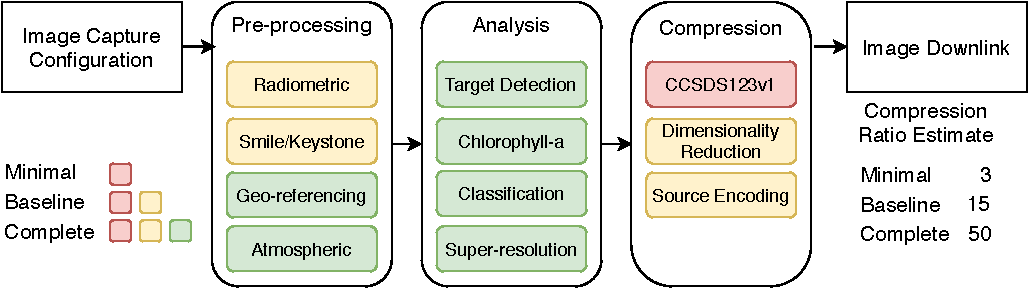
\includegraphics[width = 0.9\textwidth]{figs/img_processing/pipeline_figure_concept_paper.pdf}
    \caption{Illustration of proposed imaging pipelines. Minimal for launch, baseline for the first updates, and complete when reached maturity.}
    \label{fig:image-processing-pipelines}
\end{figure*}

\subsection{Image processing architecture}

A modular image processing pipeline enables HYPSO to downlink the minimal data product, while also permitting the satellite to downlink highly processed and reduced but relevant data (figure \ref{fig:image-processing-pipelines}).
Modules can be interchanged to create new operational data products.
Moreover, different hardware can be utilized for different components of the pipeline. 
For example, compression algorithms, based on the CCSDS123v1 standard, have been developed to run on both the CPU and the FPGA \cite{Fjeldtvedt2018}. 
While the FPGA implementation is faster, the CPU implementation allows for lossy compression, which can increase the data throughput. 
The modular design thus allows the operators to switch between the modules as needed (and the module processing configuration will be stored in the metadata for a particular image). 
However, several specific orderings of the modules are designated as target pipelines in order to maintain constistency among the data products.
Note that $12\times$ binning is incorporated into the image acquisition itself, so the most raw data is reduced before the image processing pipelines begin.
Three of the target pipelines are discussed below. 

% The planned on-board processing is divided into multiple different pipelines, illustrated in figure \ref{fig:image-processing-pipelines}, that share a basic structure, i.e. some level of processing has to be performed regardless, while others may only improve the timeliness of desired data products or reduce the expected data volume to be down-linked. In the subsequent section a high-level description of the software used and planned in the on-board processing is provided.
% \subsubsection{Settings \& Pre-processing}
% The HSI camera will collect spectrograms at a rate of 15-40 Hz. 
% The data rate is limited by the GigE that connects the camera to the breakout board, but by reducing the area of interest or doing sub-sampling in the spectral dimension, the rate at which frames are collected is adjusted \cite{varntresk2019assembly}. 
% It is expected that the imaging sensor of the HSI camera will have some distortions as a result of the optics, and that the sensitivity of given pixels will change over time. 
% Pre-processing, the initial stage of the imaging pipeline seeks to accommodate these undesirable artifacts.

\begin{table*}[htbp]
	\caption{Uncompressed Data Products*}
	\label{tab:data-products}
	\centering
	\begin{tabular}{l | r r r r}
	\hline
	& bands & pixel size (bits) & signatures (MB) & total (MB) \\
	\hline
	Raw & 1200 & $16$& - &984\hspace{10 pt} \hspace{1 pt} \\
	Binned & 100 & $16$ & - & 82.0\hspace{4 pt} \hspace{1 pt} \\
	Dim. reduced & 20 & $16$ & - & 16.4\hspace{4 pt} \hspace{1 pt} \\
	Classification (16 classes) & 1 & $4$ & 0.003 & 0.41 \hspace{1 pt} \\
	Classification (256 classes) & 1 & $8$ & 0.051 & 0.88 \hspace{1 pt} \\
	Target detection (only ACE) & 1 & $16$ & - & 0.82 \hspace{1 pt} \\
	Target detection (with abundance) & 2 & $16$ & - & 1.64 \hspace{1 pt} \\
	Target coordinates (top 100) & n/a & $16$ & - & 0.001 \\
	\hline
	\end{tabular}
	
	\begin{tabular}{c}
		*assuming 1139$\times$720 spatial pixels. \hl{what about spatial compression - jpeg?}
	\end{tabular}
	\vspace*{-\baselineskip}

\end{table*}

\subsubsection{Minimal on-board image processing}
\hl{Joe, Sivert \\}
The minimal on-board image processing pipeline (MOBIP) configuration of the image processing pipeline will typically reduce the size of the data by a factor of 2.5 or more and demonstrate the capability of on-board image processing. 
It consists of image acquisition, compression, and downlinking of the data. 
The compression is implemented on the FPGA of the OPU \cite{Fjeldtvedt2018, orlandic_parallel_2019}. 
Although it is simple, this pipeline forms the basis for all the others. 

\subsubsection{Baseline on-board image processing pipeline}
\hl{Joe, Sivert \\}
The baseline on-board image processing pipeline (BOBIP) configuration adds two important components to MOBIP, before lossless compression. The first of these is a smile and keystone correction, which adjusts the data to account for systematic measurement errors inherent to the imager \cite{Henriksen2019}. 
The second of these is dimensionality reduction, which allows for control of the size of the data package while retaining most of the information of the image. 
The smile and keystone correction is applied before the dimensionality reduction to prevent the dimensionality reduction from modeling systematic, but reversible artifacts from becoming irrevocably intertwined with the data. 

The On-the-Fly-Processing (OTFP) algorithm can be used as dimensionality reduction in order to summarize the spectral information with minimal loss of useful systematic information while simultaneously improving SNR \cite{Vit17}. 
The size of the data package can be controlled by adjusting the number of OTFP bands which are downlinked. 
Thus smile and keystone correction precedes it to avoid imprinting systematic artifacts into the reduced data. 
The residuals from the dimensionality reduction can be down-linked and analysed to provide insight as to what kind of information is being reduced away \cite{Vit17}.
Once it is tested, the BOBIP pipeline will become the standard data format. 
Moreover, dimensionality reduction will increase the speed of modules placed after it in a pipeline because there will be fewer bands to process \cite{Bakken2019SPIE}. 

\subsubsection{Target detection on-board image processing pipeline}
\hl{Joe, Sivert \\}
Another way to expand MOBIP is to add a target detection (TD) module before compression. 
Hyperspectral data is amenable to target detection because of its numerous imaging channels.
By incorporating spectral information about the background scene, TD algorithms can locate sub-pixel spectral signatures. 
The 2D heat maps produced by TD are small enough to downlink data quickly (table \ref{tab:data-types}), and can be immediately used to guide in-situ agents without requiring additional processing on the ground. \hl{Make explicit in Table IV}

The Adaptive Cosine Estimator (ACE) is a target detection algorithm in hyperspectral data that is often used to determine how likely it is that a pixel contains a particular spectral signature \cite{Manolakis2002, Manolakis2005}.
Both software and software-hardware co-design versions of the algorithm have been developed for OPU. 
Acceleration on the FPGA results in a speedup factor of about 28$\times$ relative to software implementations \cite{dijehw19_meco}. 
Effective use of ACE requires spectral knowledge about the targets to be observed. 
A spectrum can either be estimated from data in the lab, which is susceptible to calibration inconsistencies between the lab camera and the satellite camera, or it can be estimated directly from the satellite data, so that the target spectrum and input data are subject to the same limitations. 
A complementary algorithm, the fraction estimator, complements ACE by determining how much of a target is in a given pixel, which leads to the 2 bands seen in table \ref{tab:data-products}. 

\subsection{Developing advanced on-board image processing pipelines}

Some algorithms are still in development, and depending on the end-user that a given pass is targeting, different data products will be desirable.
As part of the reconfigurability of OPU, these future processing pipelines could become a part of the on-going mission. 
These algorithms include image registration, geo-referencing, atmospheric corrections, super-resolution, and classification. 
Several of these kinds of algorithms utilize the RGB camera in addition to the HSI, so it must be drawn into the image processing pipelines. 

Super-resolution algorithms are being adapted to enhance the spatial resolution of remotely sensed images \cite{Park2003, Garrett2019} and to provide improved detectability of features of interest in turn. \hl{this should be emphasized and written about further - crucial for slew maneuver and the core of this paper}
%The latter may give more accurate classification and target detection with fine spatial resolution and high spectral resolution in the image \cite{Manolakis2002, Manolakis2005, Bakken2019SPIE}.


\subsubsection{Upload/reprogram Capability (TENTATIVE)}
\hl{Joe, Sivert \\}
Both the software and FPGA configurations are planned to be updated during the operation of the satellite \cite{Gjersund2020}. First, the software update must be stringently tested on the ground, both in terms of timelinesss and resource usage. Then it must be uplinked to the satellite, which can take several passes. The payload will retain a \textit{golden image}, a version of the operating system and software known to have worked, that it will revert to in case of an update failure. 

\subsubsection{Ground Processing Pipeline}
\hl{Joe, Sivert \\}
An additional image processing pipeline should operate on the ground to (1) prepare data for end users, (2) assist in calibrating the camera in-flight, and (3) to test algorithms before uploading them to the satellite for on-board image processing. 
Some of the components of the pipeline such as geo-referencing and super-resolution are also amenable to being applied to the data after downlinking because they either require access to refence libraries or are computationally intensive.























% \hl{I'm rewriting everything that comes after this - J}

% Readily compressed and reduced data containing the relevant information across geo-referenced coordinates may efficiently be transmitted to ground enabling faster operational response to investigate target(s) of interest in-situ.

% CCSDS123 compression techniques on Field-Programmable-Gate-Array (FPGA) have proven useful for real-time processing and relatively fast lossless data-reduction of large hyperspectral data \cite{Fjeldtvedt2018}.



% \begin{table*}[]
% \begin{tabular}{lllll}
% \textbf{Method}           & \textbf{Purpose} & \textbf{Pipeline} & \textbf{Description}                                      & \textbf{Compression Factor} \\ \hline
% Radiometric Calibration   & Pre-processing   & Baseline          & Ensure correct radiometric intensities in the spectograms & N/A                         \\
% Smile/Keystone Correction & Pre-processing   & Baseline          & Correct for smile and keystone in the spectrograms        & N/A                         \\
% Atmospheric Correction    & Pre-processing   & Complete          & Correct for atmospheric effect on transmitted spectra     & N/A                         \\
% Geo-Refrencing            & Pre-processing   & Compelete         & Correlate each pixel with a location                      & N/A                         \\
% Dimensionality Reduction  & Pre-processing   & Baseline          & Denoising of image cube, data reduction                   & num\_spectra/num\_loadings  \\
% Super-Resolution          & Analysis         & Complete          & Increase spatial resolution of aquired image cube         & TBD                         \\
% Target Detection          & Analysis         & Complete          & Probability map of target                                 & num\_spectra/num\_targets   \\
% Chlorophyll-a             & Analysis         & Complete          & Estimate the chl-a content in an area                     & num\_spectra                \\
% Classification            & Analysis         & Complete          & Divide the data into spectrally distinct classes          & num\_spectra/num\_classes   \\
% CCSDS123v1                & Compression      & Minimal           & Lossless compression of image cube                        & $\sim$3                     \\
% Dimensionality Reduction  & Compression      & Baseline          & Lossy compression of image cube                           & num\_spectra/num\_loadings  \\
% Source Encoding           & Compression      & Baseline          & Lossless compression of data for transmission             & TBD                        
% \end{tabular}
% \end{table*}







\section{Conclusions} \label{sec:conclusions}
% Ocean color remote sensing is important for understanding the wellbeing of worldwide ecosystems and maritime environment. Spontaneous Harmful Algal Blooms are colorful processes with large spatial extent. These frequently cause detrimental effects on environment and sustainable aquacultural resources thus demanding high-resolution data from selected target areas that are quickly delivered after detection. Observing such phenomena requires low data latency and high spectral, spatial and temporal resolution. 
The HYPSO-1 mission and systems design shows that COTS-built hyperspectral imagers can be implemented in small-satellites for ocean color remote sensing applications, thus decreasing the development time and lowering costs for such missions. If used appropriately and with the capability of on-board image processing, these type of imagers may provide data products with sufficiently high spatial and spectral resolution as well as low latency to end users from for example the ocean color community or aquaculture industry. 
% Pushbroom hyperspectral imaging produces lines of pixels with numerous narrow spectral bands where the spatial resolution in the images may be improved by utilizing a small-satellites' ability to perform a slew maneuver during image acquisition.

Pushbroom hyperspectral imaging on a small-satellite have challenges in obtaining adequate image quality due to the smaller optics but can be amended by utilizing the small-satellite's system capabilities, in particular by rotating the camera's footprint by performing a smooth slew maneuver to improve the spatial resolution and increase the effective Signal-to-Noise Ratio (SNR) as more overlapping frames are obtained. The figures of merit presented in this paper such as optics size, spatial resolution, spectral resolution, swath width, SNR, Sequential Ground Sampling Distance, data latency as well as spacecraft angular velocity and attitude accuracy, can be used for systems trade-off studies in preliminary systems design of a spacecraft mission. This ultimately enables better efficiency in mission operations and higher performance of small space-based camera systems. 

Tailored image processing pipelines running on a FPGA on-board HYPSO-1, that include CCSDS123v1 lossless compression, dimensionality reduction, target detection, and classification, may reduce the data size considerably without losing important information and resolution. This enables quick download of the data to satisfy any immediate need of the end user, while relieving the power budget. Data products shall be validated by in-situ measurements from autonomous aerial, surface and underwater vehicles and may also be used to guide these to interesting locations. Advanced image processing algorithms under development, such as image registration, geo-referencing, atmospheric correction, super-resolution and chlorophyll estimation, shall be uploaded to the HYPSO-1's reprogrammable FPGA once in orbit. Based on lessons learned from the HYPSO-1 mission, the image processing pipelines will have enhanced and extended capabilities along with better design iterations on the hyperspectral imager for a prospective HYPSO-2 mission and a constellation of dedicated hyperspectral imaging satellites. 
\section*{Acknowledgments}
This work was supported by the Research Council of Norway, Statoil, DNV GL and Sintef through the Centers of Excellence funding scheme, Grant 223254 - Center for Autonomous Marine Operations and Systems (AMOS) and the Research Council of Norway through the IKTPLUSS programme grant 270959 (MASSIVE). This work is also supported by the Norwegian Space Centre contract SAT.01.17.7. JLG acknowledges funding from the European Research Council on Informatics and Mathematics (ERCIM) postdoctoral fellowship.

The authors would like to thank Raphe Kudela at the Ocean Sciences Department, University of California Santa Cruz, Rick Stumpf at National Oceanic and Atmospheric Administration (NOAA) and Ajit Subramaniam at the Lamont-Doherty Observatory, Columbia University for their guidance and valuable discussions on the concept. Authors would also like to thank Geir Johnsen at Department of Biology, NTNU, for his review on the remote sensing requirements, Torbjørn Skauli at Norwegian Defense Research Establishment (FFI) for his review on  practical spectroscopy, Fernando Aguado Agelet at the Department of Telecommunications Engineering, University of Vigo, and Cecilia Haskins at Department of Mechanical Engineering, NTNU, for their input on systems engineering in the project, Annette Stahl and Dennis Langer at Department of Engineering Cybernetics, NTNU, for their input on image processing, Gara Quintana for her help on radio communications and developing link budgets, and Harald Martens and Petter Rossvoll at IdleTechs for their recommendations on hyperspectral data size reduction. 
%Authors are also  grateful for the HSI mechanical design work by Tord, Tuan and Henrik as part of their Master theses at Department of Mechanical Engineering, NTNU.

\bibliographystyle{IEEEtran}
\bibliography{Reference}

\end{document}